% vim:ts=4:sw=4
%
% Copyright (c) 2008-2009 solvethis
% Copyright (c) 2010-2015 Casper Ti. Vector
% Public domain.
%
% 使用前请先仔细阅读 impthss 和 biblatex-caspervector 的文档,
% 特别是其中的 FAQ 部分和用红色强调的部分。
% 两者可在终端/命令提示符中用
%   texdoc impthss
%   texdoc biblatex-caspervector
% 调出。

% 采用了自定义的(包括大小写不同于原文件的)字体文件名,
% 并改动 ctex.cfg 等配置文件的用户请自行加入 nofonts 选项;
% 其它用户不用加入 nofonts 选项,加入之后反而会产生错误。
%
% 图书馆要求电子版论文的目录必须为黑色,
% 且某些教务要求打印版论文的文字部分为纯黑色而非灰度打印,
% 【因此最终打印和提交论文前,请将“colorlinks”改为“nocolorlinks”。】
\documentclass[UTF8, nocolorlinks, openany, spacing, pdftoc, pkuspace]{impthss}
% 设置行距为1.5。ctex说明文档中说linespread也可以作为选项传入,但测试结果显示不起效果。
% 因此在此处显示调用\linespread命令设置行距,测试显示有效果。
\linespread{1.5}
% 使用 biblatex 排版参考文献,并规定其格式(详见 biblatex-caspervector 的文档)。
% 这里按照英文文献在前,中文文献在后排序(“sorting = ecnty”);
% 若需按照中文文献在前,英文文献在后排序,请设置“sorting = centy”;
% 若需按照引用顺序排序,请设置“sorting = none”。
\usepackage[backend = biber, style = caspervector, utf8, sorting = none]{biblatex}
% 提供近似于学校所要求的 Times New Roman / Arial 的字体。
\usepackage[defaultsups]{newtxtext}
\usepackage{newtxmath}
% 产生 originauth.tex 里的 \square。
\usepackage{latexsym}

% 按学校要求设定参考文献列表中的条目之内及之间的距离。
\setlength{\bibitemsep}{3bp}
% 对于 linespread 值的计算过程有兴趣的同学可以参考 impthss-extra.sty。
\renewcommand*{\bibfont}{\zihao{5}\linespread{1.27}\selectfont}

% 设定文档的基本信息。
% \ctexset{today=big}
\impthssinfo{
	cthesisname = {博士研究生学位论文}, ethesisname = {Doctor Thesis},
	ctitle = {用于空间暗物质探测的塑闪阵列探测器的设计与研制},
	etitle = {Design and development of a plastic scintillator detector for the dark matter search in space},
	cauthor = {周勇},
	eauthor = {Zhou Yong},
	studentid = {0123456789},
	date = {\today},
	school = {中国科学院大学研究生院},
	cmajor = {粒子物理与原子核物理}, emajor = {Nuclear and Particle Physics},
	direction = {实验核物理},
	cmentor = {孙志宇教授}, ementor = {Prof.\ Sun Zhiyu},
	ckeywords = {暗物质,塑料闪烁体,PSD, DAMPE, 大动态范围,宇宙线标定,光电倍增管}, 
	ekeywords = {dark matter, plastic scintillator, PSD, DMAPE, large dynamic range, photomultiplier}
}
% 载入参考文献数据库(注意不要省略“.bib”)。
%\addbibresource{thesis.bib}
\addbibresource{./refs/ch1.bib}
\addbibresource{./refs/ch2.bib}
\addbibresource{./refs/ch3.bib}
\addbibresource{./refs/ch4.bib}
\addbibresource{./refs/ch5.bib}
\addbibresource{./refs/ch6.bib}
\addbibresource{./refs/ch7.bib}
% extra packages
\usepackage[absolute, overlay]{textpos} %封面制作
% \usepackage{import} % 使用\import,\subimport命令模块化文档结构,可以用相对路径载入文档
\usepackage{blindtext}
\usepackage{comment}
\usepackage{siunitx}
\usepackage{float}
\usepackage{mdwlist}
% \usepackage{subcaption} //error
% 表格内角注
\usepackage{threeparttable}
\AtBeginEnvironment{tablenotes}{\small}{}{}
% 设置表格字体大小
\usepackage[font=normalsize]{caption}
\let\oldtabular\tabular 
\renewcommand{\tabular}{\small\oldtabular}

\raggedbottom
\begin{comment}
	\usepackage{etoolbox}
	\newskip\mfilskip
	\mfilskip=0pt plus 3cm\relax
	\newcommand{\mfilbreak}{\vspace{\mfilskip}\penalty -200%
	\ifdim\lastskip<\mfilskip\vspace{-\lastskip}\else\vspace{-\mfilskip}\fi}
	\pretocmd{\section}{\mfilbreak}{}{}content...
\end{comment}

% 处理tiff图片
% \usepackage{grfext}
% \DeclareGraphicsRule{.tif}{png}{.png}%
% {%
  % `convert #1 `dirname #1`/`basename #1 .tif`-tif-converted-to.png %
% }

% \includeonly{./chap/introduction/introduction}
% \includeonly{./chap/description/description}
% \includeonly{./chap/dynamic_range/dynamic_range}
% \includeonly{./chap/introduction/introduction,./chap/conclusion/conclusion}

\begin{document}
	%%%%%%%%%%%%%%%%%%%%%%%%%
	%%% 封面,版权,声明,致谢 %%%
	\covermatter
	% 自动生成封面。
%	\maketitle
	% 从pdf载入封面
 	\begin{textblock*}{210mm}(0mm, 0mm)
\begin{figure*}[!hbt]
	\centering
	
\includegraphics[width=210mm]{fig/ucas_cover_cn.eps}
\end{figure*}
\end{textblock*}

 	\null\newpage
 	\begin{textblock*}{210mm}(0mm, 0mm)
\begin{figure*}[!hbt]
	\centering
	
\includegraphics[width=210mm]{fig/cover_en.eps}
\end{figure*}
\end{textblock*}


 	\null\newpage

	% 版权声明。
	% vim:ts=4:sw=4
%
% Copyright (c) 2008-2009 solvethis
% Copyright (c) 2010-2015 Casper Ti. Vector
% All rights reserved.
%
% Redistribution and use in source and binary forms, with or without
% modification, are permitted provided that the following conditions are
% met:
%
% * Redistributions of source code must retain the above copyright notice,
%   this list of conditions and the following disclaimer.
% * Redistributions in binary form must reproduce the above copyright
%   notice, this list of conditions and the following disclaimer in the
%   documentation and/or other materials provided with the distribution.
% * Neither the name of Peking University nor the names of its contributors
%   may be used to endorse or promote products derived from this software
%   without specific prior written permission.
%
% THIS SOFTWARE IS PROVIDED BY THE COPYRIGHT HOLDERS AND CONTRIBUTORS "AS
% IS" AND ANY EXPRESS OR IMPLIED WARRANTIES, INCLUDING, BUT NOT LIMITED TO,
% THE IMPLIED WARRANTIES OF MERCHANTABILITY AND FITNESS FOR A PARTICULAR
% PURPOSE ARE DISCLAIMED. IN NO EVENT SHALL THE COPYRIGHT HOLDER OR
% CONTRIBUTORS BE LIABLE FOR ANY DIRECT, INDIRECT, INCIDENTAL, SPECIAL,
% EXEMPLARY, OR CONSEQUENTIAL DAMAGES (INCLUDING, BUT NOT LIMITED TO,
% PROCUREMENT OF SUBSTITUTE GOODS OR SERVICES; LOSS OF USE, DATA, OR
% PROFITS; OR BUSINESS INTERRUPTION) HOWEVER CAUSED AND ON ANY THEORY OF
% LIABILITY, WHETHER IN CONTRACT, STRICT LIABILITY, OR TORT (INCLUDING
% NEGLIGENCE OR OTHERWISE) ARISING IN ANY WAY OUT OF THE USE OF THIS
% SOFTWARE, EVEN IF ADVISED OF THE POSSIBILITY OF SUCH DAMAGE.


\chapter*{版权声明}
% \markboth{版权声明}{} 
\thispagestyle{empty} %覆盖\chapter*{}中的调用的\thispagestyle{plain},因为此页不需要页眉页脚

任何收存和保管本论文各种版本的单位和个人,
未经本论文作者同意,不得将本论文转借他人,
亦不得随意复制、抄录、拍照或以任何方式传播。
否则一旦引起有碍作者著作权之问题,将可能承担法律责任。

% 若需排版二维码,请将二维码图片重命名为“barcode”,
% 转为合适的图片格式,并放在当前目录下,然后去掉下面 3 行的注释。
%\vfill\noindent
%\includegraphics[height = 5em]{barcode}


	% 原创性声明和使用授权说明。
	% vim:ts=4:sw=4
%
% Copyright (c) 2008-2009 solvethis
% Copyright (c) 2010-2015 Casper Ti. Vector
% All rights reserved.
%
% Redistribution and use in source and binary forms, with or without
% modification, are permitted provided that the following conditions are
% met:
%
% * Redistributions of source code must retain the above copyright notice,
%   this list of conditions and the following disclaimer.
% * Redistributions in binary form must reproduce the above copyright
%   notice, this list of conditions and the following disclaimer in the
%   documentation and/or other materials provided with the distribution.
% * Neither the name of Peking University nor the names of its contributors
%   may be used to endorse or promote products derived from this software
%   without specific prior written permission.
%
% THIS SOFTWARE IS PROVIDED BY THE COPYRIGHT HOLDERS AND CONTRIBUTORS "AS
% IS" AND ANY EXPRESS OR IMPLIED WARRANTIES, INCLUDING, BUT NOT LIMITED TO,
% THE IMPLIED WARRANTIES OF MERCHANTABILITY AND FITNESS FOR A PARTICULAR
% PURPOSE ARE DISCLAIMED. IN NO EVENT SHALL THE COPYRIGHT HOLDER OR
% CONTRIBUTORS BE LIABLE FOR ANY DIRECT, INDIRECT, INCIDENTAL, SPECIAL,
% EXEMPLARY, OR CONSEQUENTIAL DAMAGES (INCLUDING, BUT NOT LIMITED TO,
% PROCUREMENT OF SUBSTITUTE GOODS OR SERVICES; LOSS OF USE, DATA, OR
% PROFITS; OR BUSINESS INTERRUPTION) HOWEVER CAUSED AND ON ANY THEORY OF
% LIABILITY, WHETHER IN CONTRACT, STRICT LIABILITY, OR TORT (INCLUDING
% NEGLIGENCE OR OTHERWISE) ARISING IN ANY WAY OUT OF THE USE OF THIS
% SOFTWARE, EVEN IF ADVISED OF THE POSSIBILITY OF SUCH DAMAGE.

{
	\CTEXsetup[
		format+ = {\centering}, beforeskip = {40bp}, afterskip = {15bp}
	]{section}

	\chapter*{北京大学学位论文原创性声明和使用授权说明}
	\thispagestyle{empty} %覆盖\chapter*{}中的调用的\thispagestyle{plain},因为此页不需要页眉页脚
	\mbox{}\vspace*{-3em}
	\section*{原创性声明}

	本人郑重声明:
	所呈交的学位论文,是本人在导师的指导下,独立进行研究工作所取得的成果。
	除文中已经注明引用的内容外,
	本论文不含任何其他个人或集体已经发表或撰写过的作品或成果。
	对本文的研究做出重要贡献的个人和集体,均已在文中以明确方式标明。
	本声明的法律结果由本人承担。
	\vskip 1em
	\rightline{%
		论文作者签名:\hspace{5em}%
		日期:\hspace{2em}年\hspace{2em}月\hspace{2em}日%
	}

	\section*{%
		学位论文使用授权说明\\[-0.33em]
		\textmd{\zihao{5}(必须装订在提交学校图书馆的印刷本)}%
	}

	本人完全了解北京大学关于收集、保存、使用学位论文的规定,即:
	\begin{itemize}
		\item 按照学校要求提交学位论文的印刷本和电子版本;
		\item 学校有权保存学位论文的印刷本和电子版,
			并提供目录检索与阅览服务,在校园网上提供服务;
		\item 学校可以采用影印、缩印、数字化或其它复制手段保存论文;
		\item 因某种特殊原因需要延迟发布学位论文电子版,
			授权学校在 $\square$\nobreakspace{}一年 / %
			$\square$\nobreakspace{}两年 / %
			$\square$\nobreakspace{}三年以后在校园网上全文发布。
	\end{itemize}
	\centerline{(保密论文在解密后遵守此规定)}
	\vskip 1em
	\rightline{%
		论文作者签名:\hspace{5em}导师签名:\hspace{5em}%
		日期:\hspace{2em}年\hspace{2em}月\hspace{2em}日%
	}

}


	% 致谢。
	% vim:ts=4:sw=4
% Copyright (c) 2014 Casper Ti. Vector
% Public domain.

\chapter*{\hypertarget{ack}{致~~谢}}
\thispagestyle{empty} %覆盖\chapter*{}中的调用的\thispagestyle{plain},因为此页不需要页眉页脚
\pdfbookmark[1]{致谢}{ack}
% 中文测试文字。

忙碌而充实的博士生涯即将结束,谨借此机会,向帮助我和鼓励我的所有人献上最诚挚的谢意。

首先,衷心地感谢我的导师孙志宇研究员。
在硕博六年的研究过程中,孙老师无论是在学习上还是生活上,都给予了我极大的关怀与支持。
正是在您的引导下,我在理论知识、实验技能、论文写作等方面受到了比较综合的训练,并逐步学会了做科研的方法。
同时,孙老师深厚的学术功底、严谨的治学态度以及勤恳的敬业精神,无一不在潜移默化中感染着我,并激励和鞭策我不 断学习、努力进取。

特别感谢我的师兄余玉洪副研究员,他不仅是我在探测器领域的启蒙老师,也给了我很多生活、学习以及事业上中肯的建议。
在将近三年的暗物质粒子探测卫星工程研制阶段,余师兄直面挑战,克服困难,体现了一个科研工作者吃苦耐劳、勇往直前的精神。
这种精神感染了我,教会我脚踏实地做事,诚诚恳恳对人,是我人生道路上一笔宝贵的财富。

感谢次级束物理研究组唐述文、王世陶、章学恒、岳柯副研究员以及科学仪器中心的段利敏研究员,他们解答我在科研工作中碰到的问题,并无私地分享他们成功的经验。

感谢暗物质粒子探测卫星塑闪阵列分系统研制团队的所有老师、同学以及工作人员,是大家的通力合作使得我们圆满完成了塑闪阵列探测器的研制工作。特别地,我要感谢次级束研究组的陈俊岭、方芳、张永杰、王兆民,核电子学组的苏弘研究员、赵红赟、孔杰、杨海波、张惊蛰,磁铁组的杨雅清研究员、杨鹏,辐射材料组的刘杰研究员。

最后,感谢我的父母对我的鼓励和支持,你们一直是我追求学业的动力。

\par\hfill
\par\hfill\textbf{周~勇\hspace{10mm}}
\par\hfill 2016年4月12日
	
	%%%%%%%%%%%%%%%%%%%%%
	%%% 中英文摘要,目录 %%%
	% 简单页眉页脚.此后内容都加入目录,并双面打印
	\frontmatter
	% 中英文摘要。
	% vim:ts=4:sw=4
% Copyright (c) 2014 Casper Ti. Vector
% Public domain.

\begin{cabstract}
% 中文测试文字。
自从1933年暗物质的概念被首次提出到现在,大量的天文观测结果证实了暗物质的存在。
今天,暗物质假说已经被天文学家们普遍接受,并在现有的大爆炸宇宙标准模型中扮演重要角色。
由于在粒子物理的标准模型中找不到符合暗物质基本性质的稳定粒子,暗物质的组成成分和粒子属性一直困扰着人们,不断地激发人们对暗物质研究的兴趣。
许多超出标准模型的新物理理论都预言了可能的暗物质候选粒子,对暗物质的探测和研究能够检验这些新的理论模型,并有可能导致物理学产生新的革命。
近年来,国际上开展了大量的暗物质探测实验,它们使用不同的探测技术手段对暗物质问题进行研究,大大加深了人们对暗物质的认知。

暗物质粒子探测卫星(DArk Matter Particle Explorer,简称DAMPE)是中国科学空间先导专项的首批四颗科学卫星之一。
它基于空间间接探测的方法,通过测量暗物质粒子湮灭或衰变产生的$TeV$量级的高能伽马射线和高能电子能谱来探测和研究暗物质粒子。
DAMPE于2015年12月17日发射升空并成功进入预定轨道,是目前国际上同类探测器中观测能段范围最宽、能量分辨率最优的空间暗物质粒子探测器。

塑闪阵列探测器(Plastic Scintillator Detector,简称PSD)是DAMPE粒子探测器的关键子探测之一,它主要有两个功能:1)协助DAMPE的BGO量能器进行$e/\gamma$鉴别;2)进行电荷测量,鉴别$Z=1\sim 20$的入射重离子种类。
本论文的主要内容围绕着PSD的设计和研制过程展开,主要有以下几个部分组成:
\begin{itemize}
  \item PSD通过测量入射粒子沉积能量的大小实现基本功能,而空间应用环境对PSD的整体设计提出了特别的要求,本文第\ref{ch:description}章对PSD的工作原理和设计进行了简单介绍。
  \item PSD采用模块化设计,由82个探测单元模块组成X、Y相互垂直的两个塑闪阵列平面。为了满足PSD的功能需求,我们估算出每个探测单元模块都需要覆盖\SI{0.1}{MIPs}到\SI{1400}{MIPs}的动态范围区间。为此,我们设计和实现了光电倍增管双打拿极引出的读出方案,并进行了详尽的宇宙线测试和重离子束流测试以验证该设计的合理性。这些工作是第\ref{ch:large_dynmaicrange}章的主要内容。
  \item 光电倍增管是影响PSD探测单元模块性能关键器件,为了得到最佳的探测器性能,往往需要对PSD的光电倍增管进行详尽地测试。为此,我们专门设计了一套批量PMT测试平台,并用该平台得到了PSD所有候选光电倍增管的增益曲线和Dy58比值增益曲线。这些工作将在第\ref{ch:pmt_test}章进行介绍。
  \item 空间实验的特殊性要求探测器各组件具有更高的稳定性和可靠性。第\ref{ch:construction}章介绍了PSD的建造过程,主要包括PMT组件和塑闪单元条组件的测试、筛选、生产以及质量控制,以及PSD的整体装配.
  \item PSD的建造完成后,需要进行完整细致的测试以得到其性能参数。我们专门设计和搭建了一套地面宇宙线标定测试平台,并使用该平台对PSD进行了长时间的宇宙线标定。第\ref{ch:cosmic_ray}章对该平台进行了介绍,同时给出了PSD的宇宙线标定的初步结果,包括基线噪声,MIP响应,能量分辨率,衰减曲线,探测效率以及位置分辨能力。
\end{itemize}


\end{cabstract}

% \cleardoublepage
\begin{eabstract}
Since first proposed by F. Zwicky in 1933, the existence of dark matter has been confirmed by a large amount of astronomical observations.
Today, the dark matter hypothesis has been generally accepted by most of the astronomical community and plays a central role in the standard model of Big Bang cosmology.
As the Standard Model of particle physics doesn't a viable dark matter candidate which posses all the basic properties of dark matter, the composition of dark matter and its particle attribution have puzzled the scientists for a long time and continue to stimulate the interest in dark matter research.
On the other hand, many new theories beyond the Standard Model have predicted new particles that turn out to be excellent dark matter candidates.
The detection and study of dark matter could be used to verify these new theory, and may even start a new revolution in physics.
In recent years, many experiments, using different kinds of detection technologies, have been carried out to study the dark matter problem.
All these efforts will help the scientists get a deeper understanding of dark matter.

The DArk Matter Particle Explorer (DAMPE) ,
\end{eabstract}


	% 自动生成目录。	
	\tableofcontents

	%%%%%%%%%%%%%%%%%
	%%% 正文各章节 %%%
	\mainmatter
	% 各章节。
	\chapter{引言}

\section{暗物质是什么}
\subsection{暗物质存在的证据:天文观测结果}

\subsection{暗物质的粒子属性:标准模型之外的物理}
暗物质的性质与组成
现有模型的拓展:SUSY supersymmetry 有暗物质候选粒子


\section{暗物质粒子的探测方法}
暗物质粒子探测是当前的科学热点, 具有重要的物理意义和前景, 世界各国都在集中人力、物力和财力研究这一问题。根据目前的技术手段, 探测暗物质粒子的方法大致可以总结为三类: 加速器直接产生法,直接探测法和间接探测法。

加速器直接产生法是发现新粒子最常用和最有效的方法。
利用加速器将粒子加速到高能量进行对撞可以模拟宇宙大爆炸初期环境, 各种新的粒子能够在对撞后产生, 其中也可能包含暗物质候选粒子。
通过对次级粒子的探测或逃逸能量(missing energy)的重建, 可以反推出新粒子的存在并在实验室环境下研究粒子的物理特性。
产生暗物质粒子需要极高的能量, 目前只有欧洲核子中心的大型强子对撞机(LHC)能够满足这个条件。
然而, LHC只能产生较轻的暗物质粒子候选粒子, 对于更重的暗物质候选粒子, 需要建造更高能量的加速器和更加强大的粒子探测器。

第二种是直接探测暗物质粒子。该方法是直接探测来自宇宙空间的暗物质粒子与(探测器上的)原子核碰撞所产生的信号。

第三种间接探测暗物质粒子。间接法是观测暗物质粒子在宇宙空间发生衰变或相互作用之后产生的稳定粒子如伽玛射线、正电子、反质子、中微子等。

\section{暗物质粒子的空间探测}
\subsection{空间探测的优势}

\subsection{国际上的研究现状}

\section{DAMPE暗物质粒子探测卫星}
暗物质粒子子探测卫星 (英文: DArk Matter Particle Explorer, 缩写: DAMPE)是中国科学院首批空间科学战略先导专项之一, 预计于2015年11月在酒泉卫星发射基地由长征二号丁运载火箭发射上空。
DAMPE粒子探测器是暗物质粒子探测卫星的主要载荷, 它是一个高精度宽能段的能谱探测器,专门用来测量空间中高能电子、高能伽玛射线和重离子的能谱和分布。
一旦成功发射, DAMPE粒子探测器将弥补我国在空间暗物质探测上的空白, 同时也将成为世界上覆盖能区最广,精度最高的空间粒子探测器之一。

\subsection{科学目标}
暗物质粒子探测卫星的科学目标可以归结为以下三个方面:
\begin{enumerate}
	\item 寻找暗物质粒子存在的证据, 这是项目的首要目标。 通过在空间高分辨、宽能段地观测高能电子和伽玛射线寻找和研究暗物质粒子,间接测定其质量、湮灭截面或者寿命等重要的物理参量,并限定暗物质粒子的空间分布,在暗物质研究这一前沿科学领域取得重大突破。
	\item 宇宙线物理研究。通过测量TeV以上的高能电子能谱来研究宇宙线起源, 通过测量TeV/核子的核素能谱来研究宇宙射线传播和加速机制。
	\item 伽玛射线天文学研究。通过观测高能伽玛射线在伽玛天文方面取得重要成果。
\end{enumerate}

DAMPE使用间接探测法来研究暗物质粒子。
根据已有的观测结果 (见上节), 高分辨观测高能伽玛射线和电子是探测暗物质粒子可能的突破点。
空间中高能电子和伽玛射线的流量与能量成反比, 且比宇宙线本底(主要是质子和氦核)低百倍以上, 因此如何进行本底抑制是能否这种方法成功的关键。

宇宙线的起源、加速传播机制是天文学中一个重要的研究课题。
高能电子在星际中传播时,会与背景光发生逆康普顿散射且受星际磁场的作用发生同步辐射而损失能量,损失能量的速度与电子能量的平方成正比。
能量越高的电子损失能量越快,所以高能电子不能够传播太远,高于1012eV的高能电子其寿命只有105年,传播距离只有1kpc。
地球附近的宇宙高能电子只能来自于附近的高能电子源,因此它被常用于研究宇宙线的起源。。
宇宙线中的高能ce


DAMPE粒子探测器本身是一个高空间分辨和能量分辨的伽玛射线望远镜,其主要观测能段超过了国际上所有空间伽玛射线望远镜,可能会有许多预见不到的科学发现。如质子衰变实验发现了天体中微子,开辟了中微子天文学这一新的科学领域,这样的例子很多。我们期望本项目观测能够发现许多人类未知的“第一次”。

\begin{table}[htb]
	\centering
	\caption{DAMPE与其它同类探测器的性能比较}
	\label{tab:ch1:dampe_comparison}
	\begin{threeparttable}
	\begin{tabulary}{\linewidth}{LCCCC}
		\toprule[1.5pt]
		  & DAMPE & AMS-02 & FERMI-LAT & CALET \\ 
		\midrule[1pt]
		Energy Range (\si{GeV}) & $5\sim10^4$ & $0.1\sim10^3$ & $0.02\sim300$ & $1\sim10^3$ \\ 
		$e/\gamma$ Energy res.@\si{GeV}(\si{\percent}) & 1.5 & 3 & 10 & 2 \\ 
		$e/\gamma$ Angular res.@\si{GeV}(\si{\degree}) & 0.1 & 0.3 & 0.1 & 0.1 \\ 
		$e/p$ Discrimination& $10^5$ & $10^5\sim10^6$ & $10^3$ & $10^5$ \\ 
		Calorimeter thickness($\Psi_0$) & 31 & 17 & 8.6 & 30 \\ 
		Geometric accep.(\si{\meter\squared\steradian}) & 0.4 & 0.09 & 1 & 0.12\tnote{*} \\ 
		\bottomrule[1.5pt] 
	\end{tabulary}
	\begin{tablenotes}
		\item[*] DAMPE
	\end{tablenotes}
	\end{threeparttable}
\end{table}
    
\subsection{性能指标}
DAMPE卫星将运行于\SI{500}{\kilo\meter}的太阳同步轨道,设计寿命大于三年。
卫星观测能段覆盖5GeV-10TeV,能量分辨优于1.5%,超过国际上所有类似探测器。可望在暗物质粒子探测和宇宙线物理这两大科学难题上取得突破!同时更好的研究伽玛射线天文学等相关重要科学问题。
\subsection{DAMPE粒子探测器的组成}
DAMPE粒子探测器由四个子探测器系统组成, 分别是塑闪阵列探测器, 硅迳迹探测器, BGO量能器和中子探测器, 见图\ref{fig:dampe_structure}。
下面分别对各子探测器进行简单的介绍。

BGO量能器(BGO Calorimeter, 简称:BGO)

塑闪阵列探测器(Plastic Scintillator Array Detector, 简称:PSD)
塑闪阵列探测器是DAMPE的关键子探测器之一,它的主要功能有两点:
\begin{enumerate}
	\item 协助BGO量能器区分光子事件和电子事件。
	\item 鉴别入射重离子的种类,作为硅阵列探测器电荷测量的备份。
\end{enumerate}

硅迳迹探测器(Silicon-Tungsten Tracker, 简称:STK)

中子探测器(Neutron Detector, 简称:NUD)

\begin{figure}
\centering
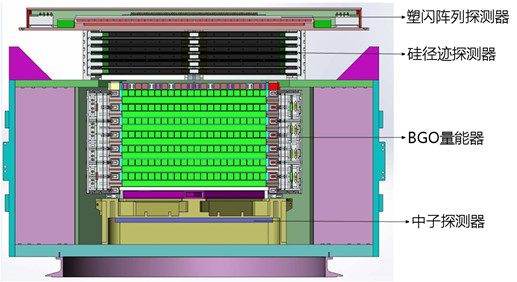
\includegraphics[width=0.8\linewidth]{chap/introduction/fig/dampe_structure_2}
\caption{DAMPE暗物质粒子探测器的整体结构}
\label{fig:dampe_structure}
\end{figure}

	% 各章节。
	\chapter{塑闪阵列探测器分系统简介}
塑闪阵列探测器(以下将简称PSD)是暗物质粒子探测卫星的关键子探测器之一,它具有两个功能:一是鉴别入射重离子(Z=1~20)的种类;二是协助BGO量能器,区分电子和光子事件。
根据实际情况,塑闪阵列探测器分系统可以分为4个功能模块,分别是塑闪阵列探测器主体功能模块、高压扇出板功能模块、前端电子学(FEE)功能模块和机械支撑功能模块。
本章将对PSD的各功能模块做一个简单的介绍,同时阐述PSD实现其粒子鉴别功能的原理以及DAMPE对PSD的性能要求。

\section{工作原理}
\label{sec:psd_principle}
有机塑料闪烁体由于具有强的抗辐照特性、快的时间响应性、好的均匀性、长的光衰减长度、光输出高且易于加工等属性,在空间探测系统中常被用于提供系统的触发信号、能量测量及飞行时间测量。
PSD选择了\SI{10}{\milli\meter}厚的有机塑料闪烁体作为探测器介质材料,并使用光电倍增管作为读出器件。
通过测量入射粒子在塑料闪烁体中的沉积能量,可以实现PSD粒子鉴别的功能,下面简要介绍一下其原理。

\subsection{重离子鉴别的原理}
\begin{figure}[h!]
	\centering
	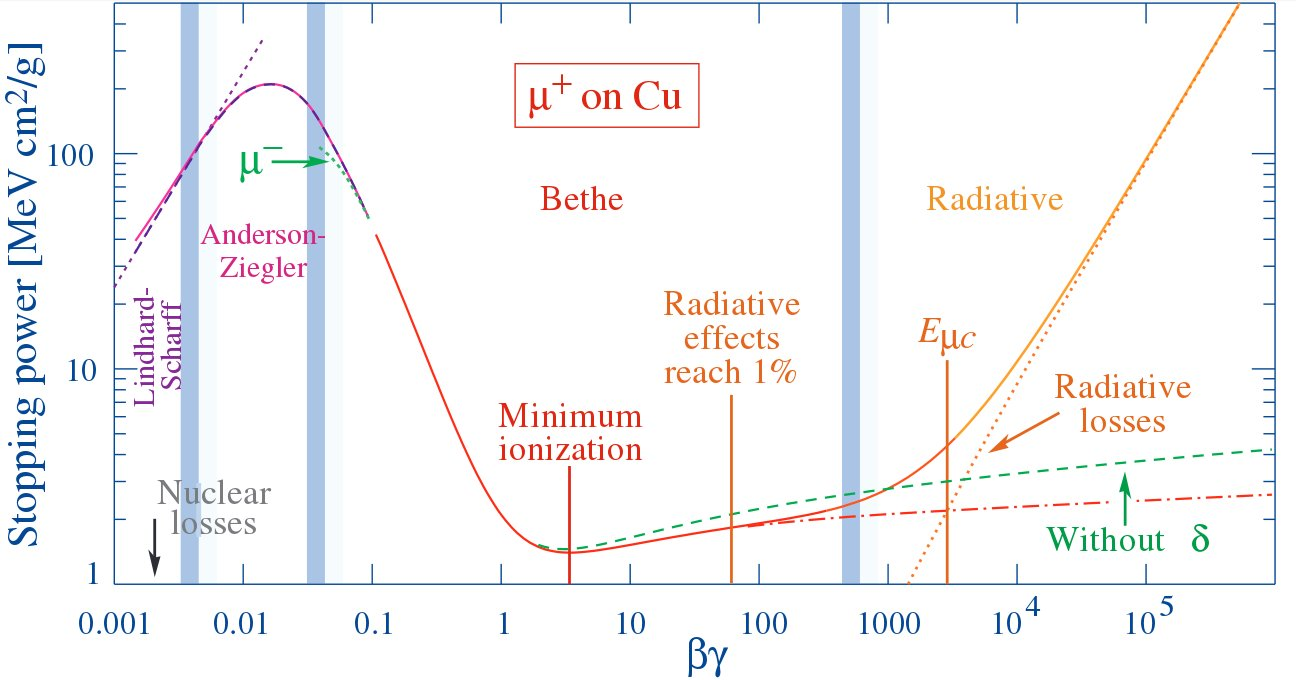
\includegraphics[width=0.8\linewidth]{chap/description/fig/energyloss_vs_velocity}
	\caption{${\mu}^+$在Cu中的能量损失率与速度的关系(用$\beta\gamma$表示),引自~\parencite{pdg_book}。 图中实线是总的能量损失率,包含了所有相互作用。}
	\label{fig:ch2:energyloss_vs_velocity}
\end{figure}

\begin{figure}[h!]
	\centering
	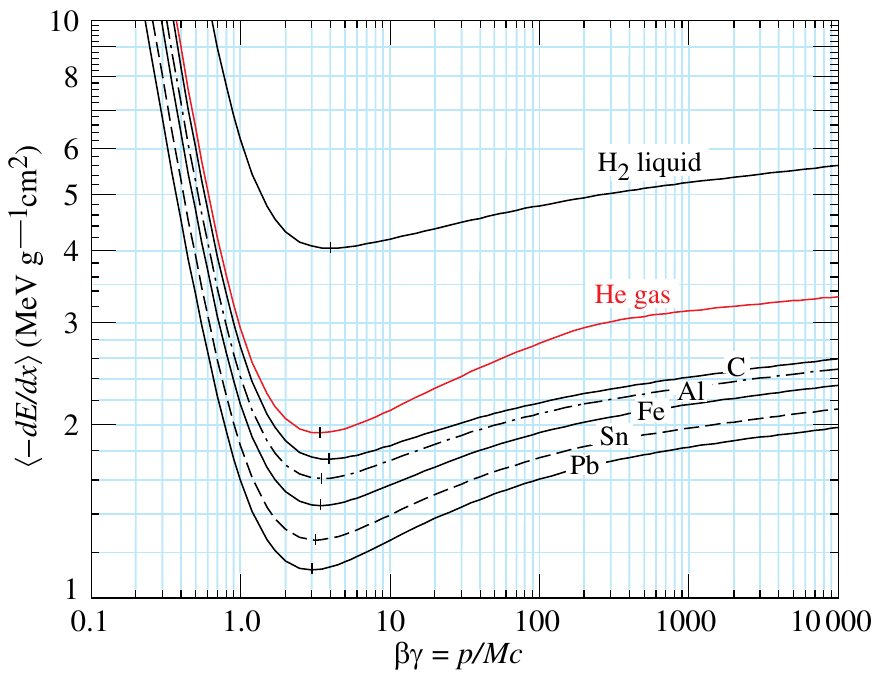
\includegraphics[width=0.8\linewidth]{chap/description/fig/fermi_plateau}
	\caption{入射粒子在几种不同介质中的电离能量损失随入射粒子动量的变化,可以清楚地看到费米坪。引自~\parencite{pdg_book}。}
	\label{fig:ch2:fermi_plateau}
\end{figure}

粒子在物质中的能量损失与其能量有紧密的关系。
对于重带电粒子(质量大于电子),其平均能量损失率与入射粒子能量的关系如图~\ref{fig:ch2:energyloss_vs_velocity}所示。
在不同能量范围内,导致能量损失的主要相互作用并不一样,图~\ref{fig:ch2:energyloss_vs_velocity}中用竖直的带子区分不同的能损区域。
DAMPE关注的能量范围属于相对论能区,此时主要是电离能损和辐射能损占主导地位。
在中等能量范围内电离相互作用起主导作用,辐射效应可以忽略;随着能量的不断升高,辐射效应逐渐不断增强,并最终其占据主导地位。
而对于重离子来说,由于其质量较大,在DAMPE的能量范围内其辐射效应不明显,因此这里只考虑它们的电离能损。

当$0.1\lessapprox\beta\gamma\lessapprox1000$($\beta=v/c,\gamma=1/\sqrt{1-{\beta}^2}$)时,重带电粒子的电离能损可以用Bethe-Bloch方程准确描述(即图~\ref{fig:ch2:energyloss_vs_velocity}中的Bethe区)):
\begin{equation}\label{eq:beth_bloch}
-\left\langle\frac{dE}{dx}\right\rangle = Kz^2\frac{Z}{A}\frac{1}{{\beta}^2}
\left[\frac{1}{2}\ln\frac{2m_ec^2{\beta}^2{\gamma}^2T_{max}}{I^2}-{\beta}^2-\frac{\delta(\beta\gamma)}{2}\right]
\end{equation}
其中$-\left\langle\frac{dE}{dx}\right\rangle$表示的是粒子通过单位约化介质层厚度的平均电离能损,K为常数,Z、A是探测器介质的原子序数和质量数,z是入射粒子的电荷数,$m_e$是电子的静止质量,c是光速,I是为介质的电离常数(也称平均激发能,有效电离电位等),$T_{max}$为入射粒子与静止的电子碰撞时传递给电子的最大动能。
$\delta$是密度效应修正项。
如图~\ref{fig:ch2:energyloss_vs_velocity}所示,在Bethe区随着入射粒子的能量由低逐渐增高时,能量损失起初像$1/{\beta}^2$一样快速减小,然后到达一个很宽范围的极小值区域。
这个极小值区域最低点约在$\beta\gamma\approx3\sim4$附近,且与介质无关。
通常将此最小值处的电离能损称为最小电离,把能量损失率为最小值的粒子称为最小电离粒子(Minimum Ionizing Particles,简称MIPs)。
在高能物理中,MIPs粒子常用来统称$z=1$的相对论性粒子(如宇宙线$\mu$子),因为它们的能量损失率与最小电离值非常接近。
经过最小电离值之后($\beta\gamma>4$),能量损失率开始缓慢上升,这是由于公式~\ref{eq:beth_bloch}方括号内第一项随$\ln{\beta}^2{\gamma}^2$变大,这个过程被称为相对论性上升。
随着能量的进一步升高,入射粒子的横向电场增强,靶核核外电子电荷密度的屏蔽效应也逐渐显著,减小了能量损失率,这种效应被称为密度效应。
密度效应在公式~\ref{eq:beth_bloch}中用$\delta/2$来表示,它使得电离能量损失率减缓并最终接近一个常数值,称为费米坪(见图~\ref{fig:ch2:fermi_plateau})。



由公式~\ref{eq:beth_bloch}可知,对同一种探测介质来说,$dE/dx$只与入射粒子的电荷量$z$和速度$\beta$有关。
对于相对论粒子来说($\beta\gamma>1$),其电离能量损失虽然与速度相关,但在很大的能量范围内其变化并不大。
因此,相对论重离子的电离能损主要取决于所带电荷量,并可以近似为:
\begin{equation}
-\left\langle\frac{dE}{dx}\right\rangle \propto z^2
\end{equation}
即与电荷量的平方成正比。
由此可见,不同种类的核素在探测器介质中的电离能损相差巨大,对于塑料闪烁体材料也一样。
因此可以通过测量PSD中沉积能量的大小进行重离子的鉴别。

\subsection{高能$e/\gamma$鉴别的原理}
\begin{figure}[h!]
	\centering
	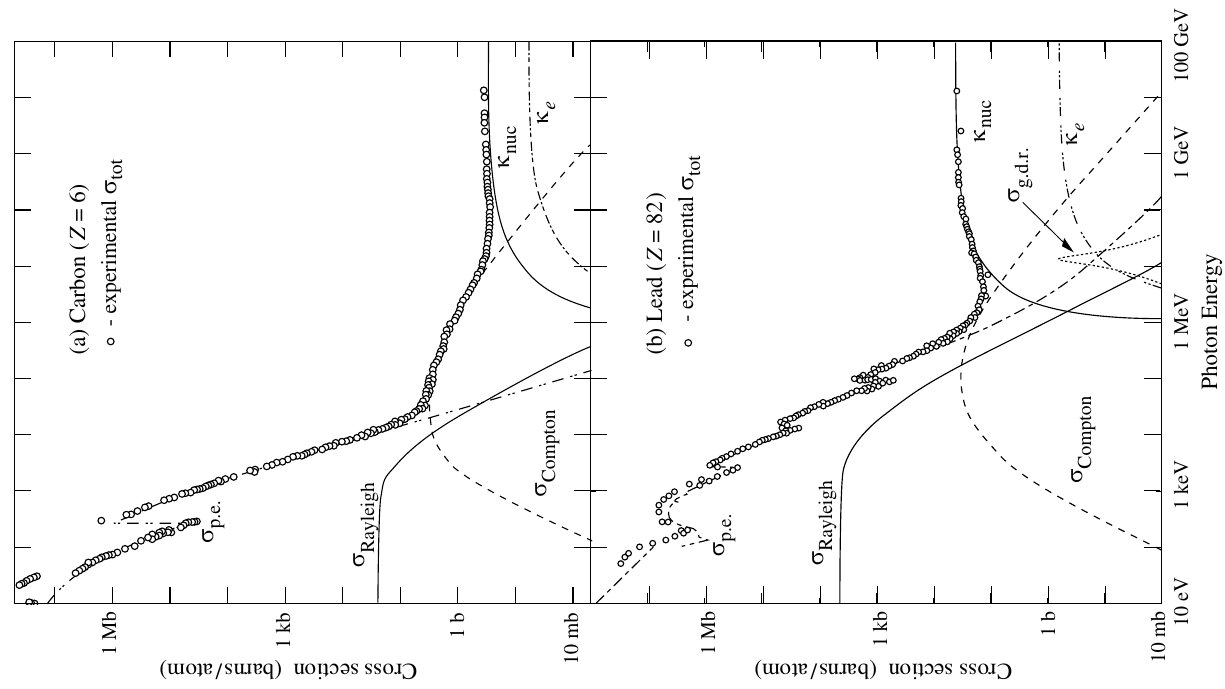
\includegraphics[width=1.2\linewidth,angle=270]{chap/description/fig/photon_energyloss}
	\caption{光子与物质各种相互作用的反应截面,上图是在碳中的,下图是在铅中的,引自~\parencite{pdg_book}。}
	\label{fig:ch2:photon_energyloss}
\end{figure}

光子可以与物质发生多种相互作用,如图~\ref{fig:ch2:photon_energyloss}所示。
其中${\sigma}_{p.e.}$是光电效应的反应截面,
${\sigma}_{Rayleigh}$是Rayleigh散射的反应截面, 
${\sigma}_{Compton}$是康普顿散射的反应截面,
${\kappa}_{nuc}$是靶核电场导致的电子对效应的反应截面,
${\kappa}_e$是靶核核外电子电场导致的电子对效应的反应截面,
${\sigma}_{g.d.r}$是光致核反应的反应截面。
在光子能量较低时光电效应占主导作用,中等能量时康普顿散射占主导作用,而高能光子一般只通过电子对效应损失能量.
从图~\ref{fig:ch2:photon_energyloss}中可以看到电子对效应的反应截面非常小,再加上PSD使用的塑料闪烁体材料密度小、厚度薄,高能$\gamma$射线在PSD中发生反应的概率非常小,因此基本不会有能量沉积。

对于电子/正电子来说,它们的质量小,在物质中的能量损失情况与重带电粒子有很大的不同。
电子/正电子与靶原子的相互作用,主要是电离能量损失,辐射能量损失和多次散射。
在能量较低时,电子/正电子虽然可以通过Møller散射,Bhabha散射和正电子湮灭损失能量,但电离能损仍然占据主导地位,见图~\ref{fig:ch2:electron_energyloss}。
随着电子/正电子能量的升高,轫致辐射效应开始显著起来,并随着能量的增大近似以线性形式增强。
电离能损随着能量的增大以对数形式增强,因此当能量大于\SI{100}{MeV}之后轫致辐射导致的能损开始占据主导地位。
在DAMPE关注的能区,穿过PSD的电子/正电子主要通过轫致辐射损失能量。
然而,高能电子/正电子轫致辐射产生的光子能量也比较高,一般不在PSD中沉积能量。
另一方面,电离相互作用虽然不占据主导作用,但它是一个连续过程,会一直在PSD中沉积能量,其大小大概与MIPs粒子的能量沉积差不多。

\begin{figure}[h!]
\centering
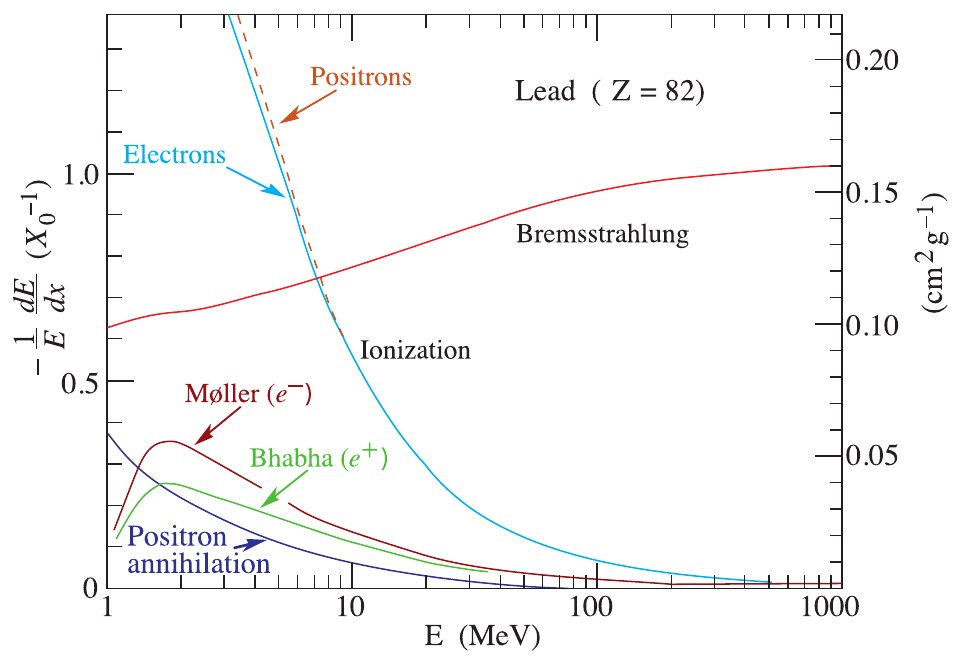
\includegraphics[width=0.8\linewidth]{chap/description/fig/electron_energyloss}
\caption{电子/正电子在铅中的单位辐射长度能损比例与能量的关系,引自~\parencite{pdg_book}。}
\label{fig:ch2:electron_energyloss}
\end{figure}

综上所述,高能光子在PSD中没有能量沉积,高能电子/正电子在PSD中有能量沉积。
根据入射粒子是否在PSD中有能量沉积,可以将光子和带电粒子区分开来;进一步结合BGO量能器,可以将电子/正电子和其它带电的强子区分开来。

\section{性能要求}
\label{sec:psd_requirements}

结合DAMPE探测器整体的物理需求,PSD需要达到的性能指标如下:
\begin{enumerate}[noitemsep,topsep=0pt]
	\item 有效探测面积$\SI{820}{\milli\meter}\times\SI{820}{\milli\meter}$。DAMPE是单方向的探测器,即它只关心从顶部入射的粒子。由于PSD位于DAMPE探测器最顶端,它的有效探测面积决定了DAMPE的视场大小。PSD是DAMPE中面积最大的子探测器。
	\item 探测单元实现电子和重离子($Z=1\sim20$)的测量。根据~\ref{sec:psd_principle}节的描述,重离子在PSD中的能量沉积相差巨大,这就对PSD探测单元提出了大动态范围的要求。另外,为了有效区分电子信号和噪声本底(光子不在PSD中产生信号),探测单元还需要由较高的信噪比(Signal to Noise Ratio,简称SNR)。因此PSD的探测单元需要进行认真地设计和验证以满足这些要求,这将在第三章进行详细讨论。
	\item 探测单元电荷分辨优于\SI{25}{\percent}($\sigma$,Z=1)。为了对不同种类的重离子进行有效鉴别,探测器分辨率需要满足一定条件。由于塑料闪烁体材料本身的限制,PSD探测探测单元的分辨率确定为对$Z=1$的粒子(对于$Z>1$的重离子,探测器响应很难在实验室条件下进行验证)的$\sigma$好于\SI{25}{\percent}。在相对论能区,所有$Z=1$的粒子与MIPs粒子具有类似的能量沉积,这个要求可以简化为对MIPs粒子的能量分辨好于\SI{25}{\percent}。
	\item 空间分辨好于\SI{2}{\centi\meter}。迳迹探测不是PSD的主要功能,DAMPE的主要迳迹探测器是STK。但在迳迹寻找和重建过程中,STK需要BGO和PSD提供额外的位置信息以便其更有效地找到并验证真实迳迹。因此,PSD的位置信息不需要特别精确,最终被确定为\SI{2}{\centi\meter}。
	\item 对MIPs粒子的探测效率高于\SI{95}{\percent}。这是$e/\gamma$鉴别提出的要求,包含两部分内容:一是对带电粒子的探测器效率高于\SI{95}{\percent},二是对光子的误判率低于\SI{5}{\percent}。
\end{enumerate}

\section{探测器主体功能模块}
\subsection{PSD整体构型}
\label{sec:psd_composition}

\begin{figure}[b!]
	\centering
	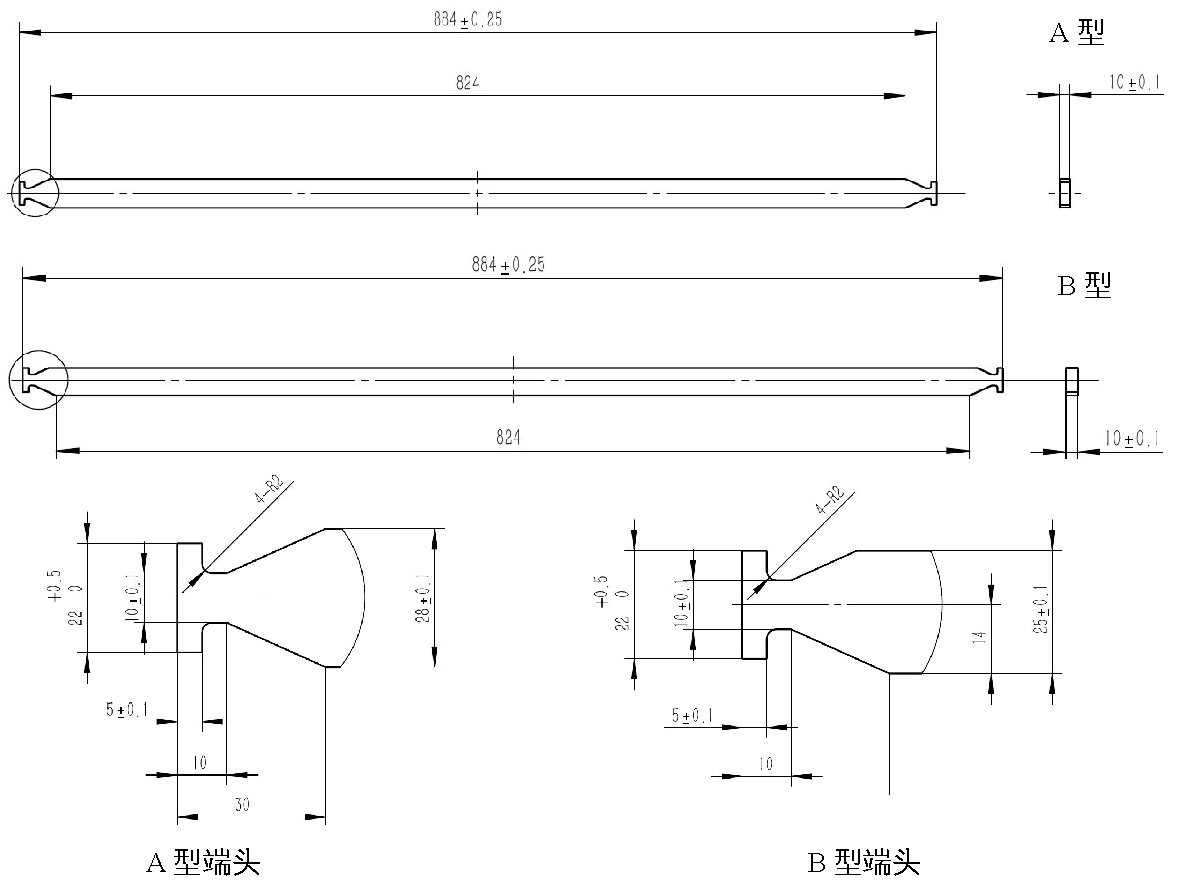
\includegraphics[width=\linewidth]{chap/description/fig/bars}
	\caption{PSD中两种塑闪单元条的尺寸}
	\label{fig:ch2:bars}
\end{figure}

入射粒子在BGO量能器中发生电磁簇射或强子簇射时,大部分次级粒子都是前向的,但也有小部分次级粒子由于大角度散射反照(backscatter)到PSD上。
反散射的簇射粒子由于带电或能量较低,在PSD上会有能量沉积,使得PSD测到的能量变大,这可能造成光子被误判为带电粒子,或者质子被误判为重离子。
为了减小由此引起的误判率,PSD采用了模块化设计,即将PSD切割成一个个足够小的探测单元,每个探测单元模块都能独立进行能损测量。
由于反散射粒子在入射粒子迳迹周围会有一个分布,且在入射粒子穿过的PSD探测单元内接收的反散射粒子最少(因为\ang{180}反散射的概率最小),如果只使用入射粒子穿过的PSD探测单元作为粒子鉴别的依据,就可以大大降低反散射簇射粒子造成的误判率。
PSD模块化带来的另一个好处是增加了一组位置信息,因为每个探测单元模块都对应一个固定的空间位置坐标。

PSD的最小探测单元是一根长度为\SI{884}{\milli\meter},厚度为\SI{10}{\milli\meter}的有机塑料闪烁体单元条。
单元条的宽度有两个规格:A型宽度为\SI{28}{\milli\meter},B型宽度为\SI{25}{\milli\meter},见图~\ref{fig:ch2:bars}。
单元条的端头被加工成特殊的“工”字形,这是为了将单元条与支撑结构更好地固定在一起(详见第~\ref{sec:psd_support}节)。
每根塑闪单元条的两端都耦合一个光电倍增管(PMT)作为读出器件,这构成了PSD的一个探测器单元模块。

\begin{figure}[h!]
	\centering
	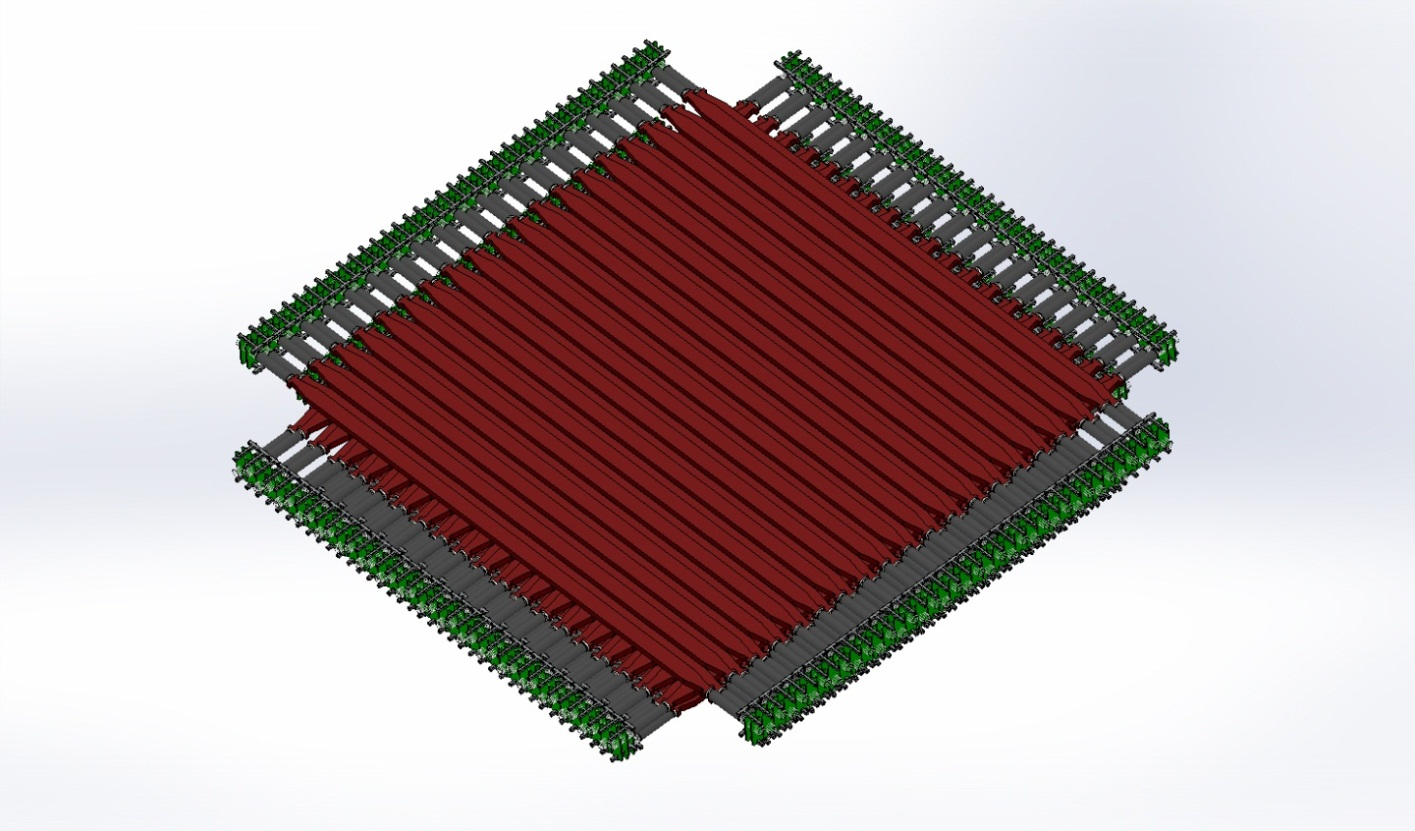
\includegraphics[width=0.72\linewidth]{chap/description/fig/psd_detector}
	\caption{PSD探测器的整体构型}
	\label{fig:ch2:psd_explosion}
\end{figure}

\begin{figure}[h!]
	\centering
	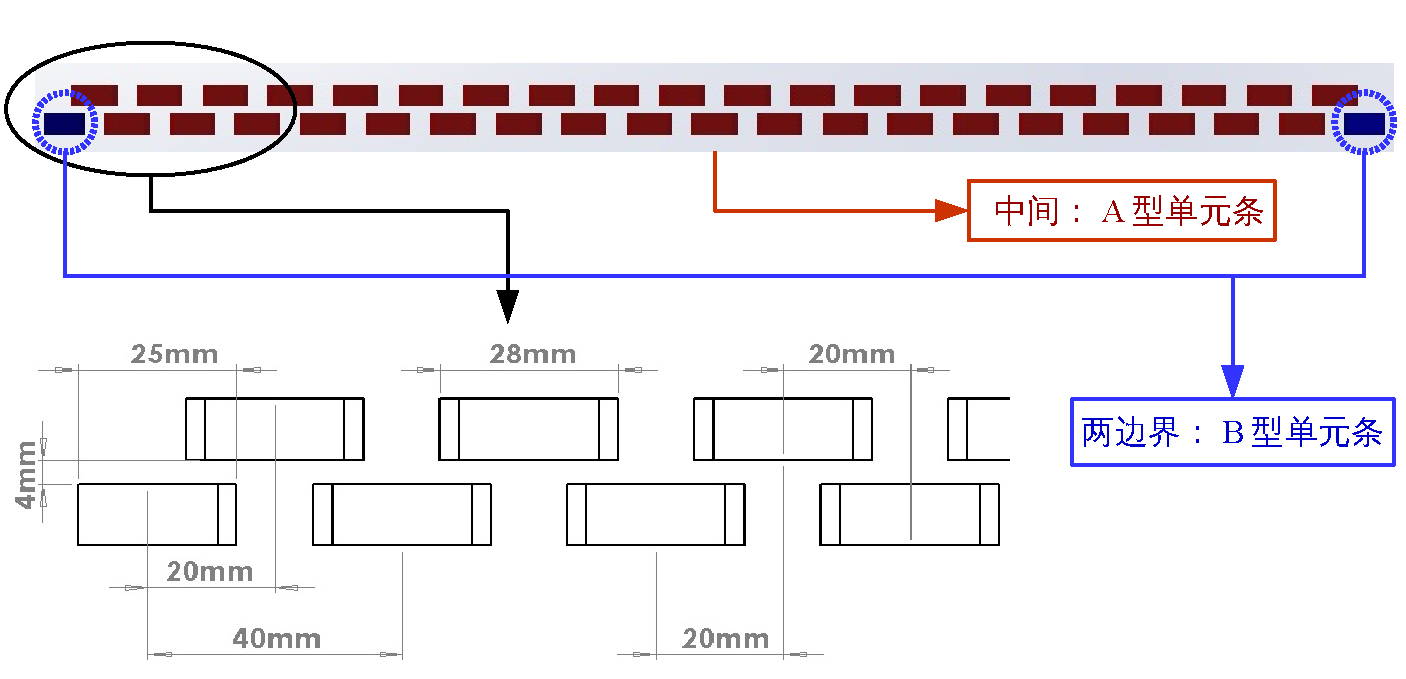
\includegraphics[width=0.8\linewidth]{chap/description/fig/bars_layout}
	\caption{塑闪阵列平面内的单元条交叠放置以消除探测器灵敏死区。}
	\label{fig:ch2:bars_layout}
\end{figure}

PSD一共由82个探测单元模块组成,分为X、Y两个相互垂直的塑闪阵列平面,见图~\ref{fig:ch2:psd_explosion}。
X、Y两个探测平面的构型完全一样,每个平面内的41个探测单元平行紧密排列,A型单元条被放置在探测平面的中间部位,B型单元条被放置在平面的两边界上。
这样,PSD一共需要使用78根A型单元条,4根B型单元条以及164支PMT。
每个探测平面内,探测单元模块交错放置成“品”字形排列用以消除相邻单元条之间的间隙(探测死区),见图~\ref{fig:ch2:bars_layout}。
相邻单元模块的中心距离为\SI{20}{\milli\meter},因此单元条的重叠区域为\SI{8}{\milli\meter},足以消除DAMPE探测器广视角造成的探测器死区。
简单计算可以得到,PSD覆盖的有效探测面积为$\SI{822}{\milli\meter}\times\SI{822}{\milli\meter}$。

\subsection{探测器单元模块}
PSD探测单元模块由一根塑闪单元条及其两端耦合的两支PMT组成。
有机塑料闪烁体将入射粒子的沉积能量成正比地转化为闪烁光子;闪烁光传输到单元条两端,被PMT收集,光电转换,倍增产生电流信号;电流信号输入到后续的前端电子学模块进行处理和模数转换,最终被记录下来。

PSD选择了Eljen公司的EJ-200~\parencite{ej-200}作为探测器介质材料,其主要性能参数参看表~\ref{tab:ch2:ej200}。
EJ-200具有空间使用经验,曾被成功的使用到AMS-02项目中。
它具有良好的抗辐照性能,经过\SI{400}{\kilo\radian}剂量的辐照后,其性能不会发生明显的变化~\parencite{ams02_tof}。
EJ-200本身具有较好的光传输性能,但由于PSD单元条的长度较长、宽度较窄,闪烁光在单元条表面会发生多次反射和折射过程而损失掉。
为了提高光传输效率,PSD塑闪单元条的表面(除了与PMT耦合的端面)进行了抛光处理,同时使用Tyvek纸对塑闪单元条主体进行包装以提高反射率。
太阳光会对PSD探测器单元模块的工作造成干扰,因此Tyvek包装层外又包裹了一层黑色热缩管材料进行避光,见图~\ref{fig:ch2:bar_wrapping}。

\begin{figure}[h!]
\centering
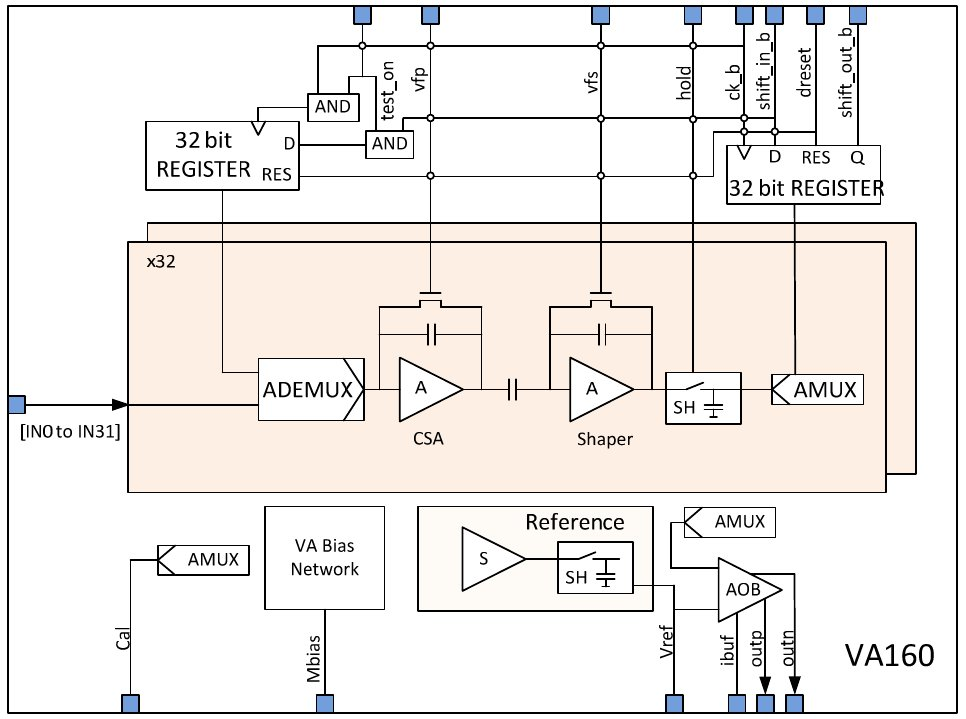
\includegraphics[width=0.8\linewidth]{chap/description/fig/va160}
\caption{PSD塑闪单元条的包装。}
\label{fig:ch2:bar_wrapping}
\end{figure}

\begin{longtabu} to 0.8\linewidth{lX}
	\caption{EJ-200的主要性能参数\label{tab:ch2:ej200}}\\
	\toprule[1.5pt]
	\textbf{性能参数} & \textbf{典型值} \\ 
	\midrule
	\endfirsthead
	
	%\toprule[1.5pt]
	\multicolumn{2}{ c }{续表~\ref{tab:ch2:ej200}}\\
	%性能参数 & 典型值 \\ 
	\midrule
	\endhead
	
	%\bottomrule[1.5pt]
	\endfoot
	
	\bottomrule[1.5pt]
	\endlastfoot
	
	H/C原子比 & 1.10 \\
	原子密度 & H: \SI{5.523E22}{\per\cubic\centi\meter}, C:\SI{4.740E22}{\per\cubic\centi\meter} \\
	光输出 & \SI{64}{\percent}(相对蒽)\footnote{\SI{60}{\celsius}时的光输出是\SI{20}{\celsius}时的\SI{95}{\percent},\SI{-60}{\celsius}$\sim$\SI{20}{\celsius}时光输出不依赖于温度} \\
	上升时间 & \SI{0.9}{\nano\second} \\
	衰减时间 & \SI{2.1}{\nano\second} \\
	光谱峰位 & \SI{425}{\nano\meter} \\
	衰减长度 & \SI{210}{\centi\meter} \\
	折射率   & 1.58 \\
	密度    &  \SI{1.032}{\g\per\cubic\centi\meter} \\
	膨胀系数 & \SI{7.8E-5}{\per\celsius} \\
	软化温度 & \SI{70}{\celsius} \\
	蒸气压   & 能用于真空 \\
	溶解性  &  可溶于芳香族溶剂、氯化溶剂及丙酮等,不溶于水、稀酸、低浓度酒精、碱及硅脂等 \\
\end{longtabu}

光电倍增管(PMT)是粒子物理实验中一种常用的光电转换器件,它具有结构简单、增益高、线性范围广以及对单光子敏感等优点。
然而,空间环境的特殊性对PMT的选择和使用提出了额外的要求,如力学性能(主要是发射阶段的振动和冲击)和磁屏蔽性能(卫星磁棒以及地球的弱磁场)。
PSD选择了Hamamatsu公司的R4443-MOD2型光电倍增管作为读出器件,表~\ref{tab:ch2:r4443}给出了它的具体性能参数。
R4443是一种端窗型、玻璃管身的光电倍增管(见图~\ref{fig:ch2:r4443_rare}),它的结构经过特殊的加固处理,能在恶劣的力学环境下工作;并且,R4443曾在GLAST项目上成功使用过,已有空间使用经历。
R4443-MOD2是R4443的升级版本,主要替换了光阴极材料,使得其暗电流大大降低,而基本结构没有改动,因此,其力学性能可以得到保证。
PSD探测器单元模块处的磁场强度小于\SI{5}{Gauss},因此R4443-MOD2外部缠绕了一层玻莫合金以消除磁场对PMT增益的影响。
使用中,为了提高可靠性,R4443-MOD2外部还设计了硅胶保护层进行力学减震,同时PMT整体将安装到特殊的保护套中并固定在探测器支撑结构上(详见第~\ref{sec:psd_support}节)。

\begin{figure}[h!]
\centering
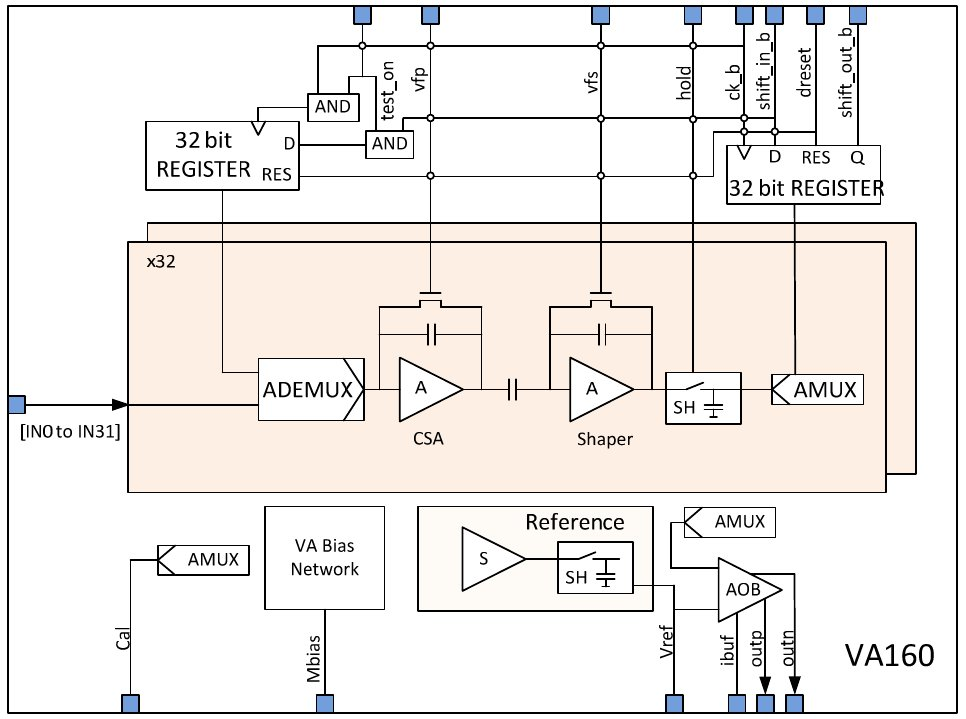
\includegraphics[width=0.8\linewidth]{chap/description/fig/va160}
\caption{R4443-MOD2裸管}
\label{fig:ch2:r4443_rare}
\end{figure}

\begin{longtabu} to 0.6\linewidth{lX}
	\caption{R4443 Mod2的主要性能参数\label{tab:ch2:r4443}}\\
	\toprule[1.5pt]
	\textbf{性能参数} & \textbf{典型值} \\ 
	\midrule
	\endfirsthead
	
	%\toprule[1.5pt]
	\multicolumn{2}{ c }{续表~\ref{tab:ch2:r4443}}\\
	%性能参数 & 典型值 \\ 
	\midrule
	\endhead
	
	%\bottomrule[1.5pt]
	\endfoot
	
	\bottomrule[1.5pt]
	\endlastfoot
	
	波长响应范围 & 300$\sim$650 \si{\nano\meter} \\
	光谱峰位 & \SI{375}{\nano\meter} \\
	光阴极材料 & 低噪声双碱金属 \\
	光阴极最小有效面积 & \SI{10}{\milli\meter} \\
	工作温度 & \SI{-30}{\celsius}$\sim$\SI{50}{\celsius} \\
	上升时间 & \SI{2.5}{\nano\second} \\
	渡越时间 & \SI{24}{\nano\second} \\
	打拿极数 & 10 \\
	典型增益 & \SI{1.0E6}{} \\
	最大工作电压 & \SI{1250}{\volt}\\
	重量 & \SI{11}{\g}\\
	外部尺寸(直径) & \num[separate-uncertainty]{14.5(7)} \si{\milli\meter} \\
	典型暗电流 & \SI{0.5}{\nano\ampere}\\
	最大暗电流 & \SI{4.0}{\nano\ampere} \\
	冲击 & \SI{5000}{\meter\per\square\second}(500 g's)\\
	振动 & \SI{200}{\meter\per\square\second}(20 g's) \\ 
\end{longtabu}

塑闪单元条与R4443-MOD2之间使用硅脂垫片直接进行耦合。
硅脂垫片材料使用的是Eljen公司的EJ-560,其性能参数见表~\ref{tab:ch2:ej560}。
硅脂垫片是一种弹性材料,可以缓冲单元条与PMT之间的刚性接触并有效释放塑闪单元条的温度形变产生的应力压迫,起到保护PMT的作用。
另外,EJ-560的折射率与PMT入射窗玻璃和塑料闪烁体的折射率非常接近,可以提高光耦合效率,将传输造成的闪烁光损失降到最低程度。

\begin{table}[htb]
	\centering
	\caption{EJ-560主要性能参数}
	\label{tab:ch2:ej560}
	
	\begin{tabulary}{0.6\linewidth}{LC}
		\toprule[1.5pt]
		\textbf{物理性能} & \textbf{典型值}                              \\ 
		\midrule[1pt]
		厚度            & \SI{3}{\milli\meter}                      \\
		密度            & \SI{1.03}{\g\per\cubic\centi\meter}       \\
		硬度(A型邵氏硬度计)   & 16$\sim$24                                \\
		折射率           & 1.43                                      \\
		工作温度范围        & \SI{-40}{\celsius}$\sim$\SI{70}{\celsius} \\
		热膨胀系数         & \SI{3E-4}{\per\celsius}                   \\ 
		\bottomrule[1.5pt]
	\end{tabulary}
	
\end{table}

\section{高压扇出功能模块}
\label{sec:psd_hv}
PSD探测单元模块的PMT高压由DAMPE的高压单机分系统提供。
由于卫星的资源限制,DAMPE高压单机不能给PSD的每个PMT提供独立的高压,多个PMT需要共享一个高压通道。
PSD高压扇出模块的功能就是将DAMPE高压单机提供的一路高压分为多路高压通道,并提供给各个PMT使用。

PSD探测器的每个侧面都配备了一块高压扇出PCB板,一共4块。
每块高压扇出板上有6个输入高压模块,负责将来自DAMPE高压单机的6路输入高压按照$7+7+7+7+7+6$的模式提供给PSD一个侧面的41支PMT使用。
DAMPE高压单机不能提供连续可调的高压值,只有8个高压档位可以使用,分别为\SI{0}{V}(小于\SI{60}{V}),\SI{780}{V},\SI{810}{V},\SI{840}{V},\SI{870}{V},\SI{900}{V},\SI{930}{V},\SI{960}{\volt}。
加上多个PMT共享一路高压,这就要求同一高压组别内的PMT需要有相似的增益和增益曲线,这个问题将在第四章详细讨论。

\section{前端电子学功能模块}
\label{sec:psd_electronics}
\begin{figure}[h!]
	\centering
	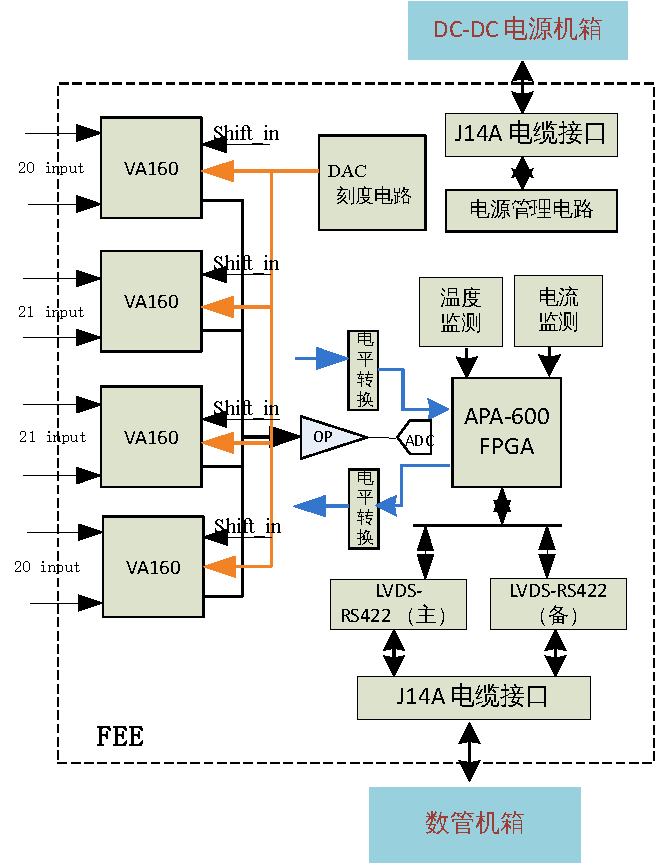
\includegraphics[width=0.7\linewidth]{chap/description/fig/psd_fee1}
	\caption{PSD的前端电子学原理框图。}
	\label{fig:ch2:psd_fee1}
\end{figure}

前端电子学功能模块是PSD的数据处理单元,它接收来自DAMPE载荷数管机箱分系统的控制信号和触发信号,产生PSD的科学数据、工程参数数据以及遥测数据,并传输到载荷数管机箱分系统中。
载荷数管是DAMPE探测器的数据处理中心,它负责与卫星的通信并协同各子探测器间的工作;来自子探测器的数据在载荷数管进行重组并被发送到载荷管理器的存储单元,等待卫星入站后由数传通道下行到地面。
PSD的前端电子学功能模块一共由4块前端电子学板(FEE)组成,每个侧面各一块,负责该面的PMT信号处理。
图~\ref{fig:ch2:psd_fee1}给出了FEE板的原理框图,FEE由以下功能电路组成:钳位保护电路、电荷测量电路、模拟调理电路、模数变换电路、刻度电路、温度/电流监测电路、FPGA及外围电路、电源管理电路以及接口电路。
下面对其主要功能做一个简单的介绍,更详细的内容参看~\parencite{yanghaibo_thesis,psd_tdr}。

\subsection{电荷测量}
电荷测量是FEE的主体功能,PSD选择了一款来自挪威IDEAS公司的ASIC(Application Specific  Integrating Circuit)芯片作为电荷测量的核心电路。
VA160是一款高集成度、低功耗、高灵敏度的电荷测量芯片(见表~\ref{tab:ch2:va160}),能够满足DAMPE卫星载荷的功耗和空间/重量限制。
另外,VA160是VA32的改进版本,而VA32在AMS-02中成功使用过,其空间抗辐照性能可以保证。

\begin{table}[h]
	\centering
	\caption{VA160的主要性能参数}
	\label{tab:ch2:va160}
	
	\begin{tabulary}{0.7\linewidth}{Ll}
		\toprule[1.5pt]
		\textbf{参数} &                     \textbf{典型值}                       \\ 
		\midrule[1pt]
		通道数         &                          32                            \\
		电荷测量范围      &           \SIrange{-3}{13}{\pico\coulomb}            \\
		成形时间        &          \SIrange{1.8}{2.3}{\micro\second}            \\
		等效噪声电荷(ENC) &       3200 \si{e} + 7.6 \si{e\per\pico\farad}          \\
		积分非线性       &                   \SI{2}{\percent}                     \\
		功耗          & 平稳工作:\SI{181}{\milli\watt},最大值:\SI{203}{\milli\watt}   \\ 
		\bottomrule[1.5pt]
	\end{tabulary}
\end{table}

\begin{figure}[h!]
	\centering
	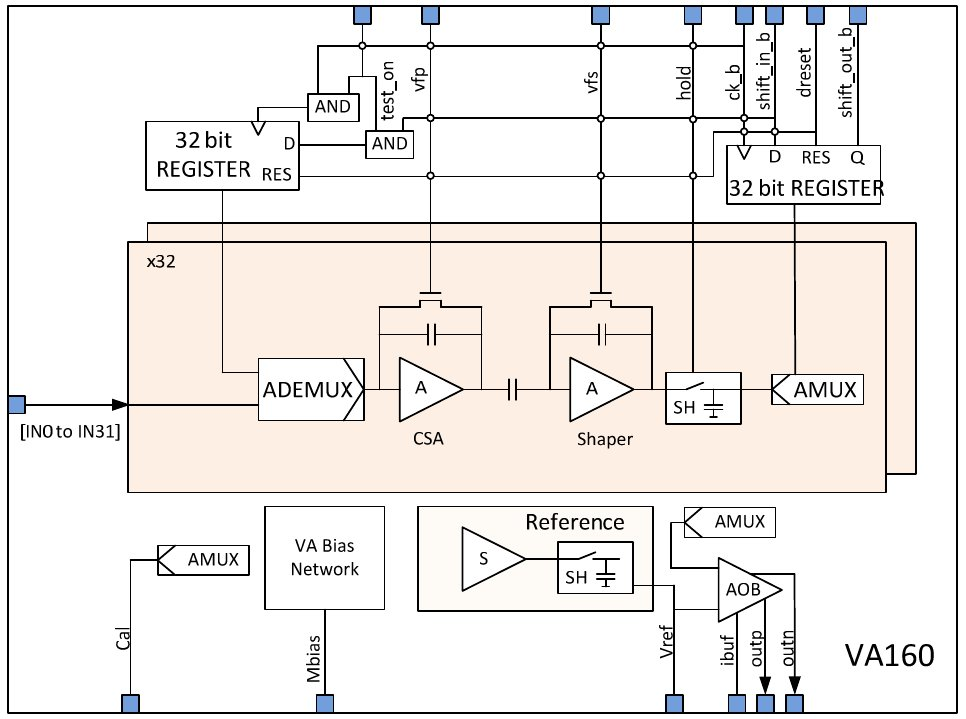
\includegraphics[width=0.8\linewidth]{chap/description/fig/va160}
	\caption{VA160原理框图,来自~\parencite{fengchangqing_eqm}}
	\label{fig:ch2:va160}
\end{figure}

图~\ref{fig:ch2:va160}给出了VA160的电路原理框图。
VA160一共有32个独立的电荷测量通道,每个测量通道都是一个完整的电荷测量电路,包括:电荷灵敏前置放大器(CSA),CR-RC成形电路(Shaper)和采样保持电路(SH)。
VA160采用电流-电荷方法进行电荷测量:来自R4443-MOD2的电流脉冲信号通过钳位保护电路直接输入到VA160中;前置放大器对输入的电流脉冲进行积分,并输出与电荷量成正比的电压;电压信号之后经耦合电容输入到成形电路中,成形后的准高斯波形在$\sim$\SI{1.8}{\micro\second}处到达峰值,且峰值大小与输入电压成正比;最后,采样保持电路在某个时刻产生一个保持信号,并将成形电路此时刻的输出电压保持住以等待后续电路的处理。
为了能够准确测量输入的电荷量,保持信号应该在成形脉冲到达峰值时产生,这样才能采到峰值电压,如图~\ref{fig:ch2:sample_hold}所示。
由于成形时间在微秒量级,DAMPE的触发信号一般在达峰之前到来,因此保持信号需要在触发信号延迟一段时间后产生。
所有测量通道最终通过一个32选1的模拟多路开关依次经过电流输出型全差分放大器输出。
VA160输出的差分电流信号经过模拟调理电路后被转换成电压信号,最后输入到一款14位的高精度ADC中进行模/数转换并被记录下来。
除了32个正常的测量通道外,VA160内还有一个悬空参考通道,用于抑制共模噪声和由温度引起的电子学漂移。

\begin{figure}[h!]	
	\centering
	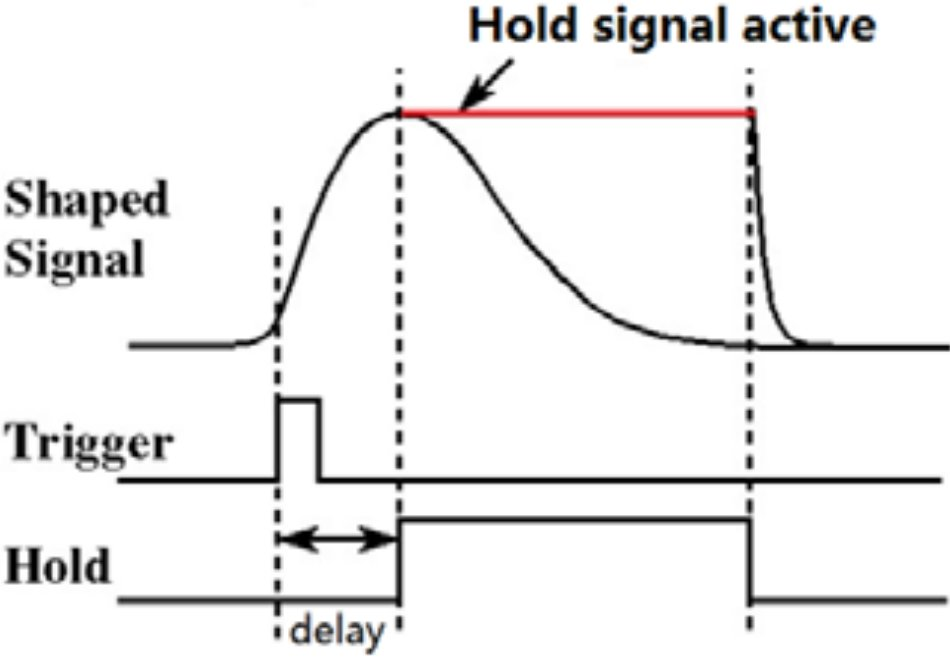
\includegraphics[width=0.5\linewidth]{chap/description/fig/sample_hold}
	\caption{保持信号与触发信号的关系。}
	\label{fig:ch2:sample_hold}
\end{figure}

PSD的每个侧面有41支PMT,由于每支PMT输出两个信号(Dy5和Dy8双打拿极输出,详见第三章),每个侧面一共有82个待测电流信号。
Dy5和Dy8的信号幅度相差较大,为了减少通道间的串扰,它们被连接到不同的VA160芯片上。
因此,每块FEE板上使用了4片VA160芯片。
另外,为了对FEE本身的电子学噪声进行监测,每片VA160额外输出2个悬空通道(冗余设计),最终每块FEE板会产生90个通道的科学数据。

\subsection{电子学刻度}
电子学刻度指的是,利用电荷量已知的脉冲信号模拟真实的信号输入,对电子学通道的性能进行标定和自检。
PSD设计了专门的电子学刻度电路,并集成在FEE板上,它具有如下几个功能:
\begin{enumerate}
	\item 为了准确测量信号电荷量,FEE的电荷测量电路(包括VA160测量通道、模拟调节电路和模/数转换)具有良好的线性。通过电子学刻度可以得到整个电子学测量通路的线性范围,同时得到非线性参数,以便进行离线修正。
	\item 在调试、运行过程中,通过了解FEE电荷测量通道的性能状态,可以发现异常状况和故障,因此电子学刻度电路兼具自检的功能。
	\item DAMPE卫星的设计寿命是3年,长时间的运行过程中,工作环境、器件老化等因素会引起电荷测量电路的参数变化。通过电子学刻度对各测量通道进行定期的标定,可以监测并修正这些参数变化,保证测量结果准确有效。
\end{enumerate}

电子学刻度的信号产生电路由模拟开关(Switch)、参考电平产生电路(DAC)、放电电阻(\SI{10}{\kilo\ohm})以及刻度电容($C_{calib}$=\SI{10}{\pico\farad})组成,如图~\ref{fig:ch2:fee_calibration}所示。
DAC输出一个恒定的参考电压$V_{ref}$,FPGA控制模拟开关的通断从而产生一个阶越的电压信号。
此时,为了使得刻度电容的电压值达到参考电压值$V_{ref}$,刻度电容两端会产生一个脉冲电流对刻度电容充电。
刻度电容左端与VA160的Cali管脚相连,因此这个脉冲电流被直接用于VA160的通道刻度,其对应的电荷量为$Q_{calib}=V_{ref}C_{calib}$。
通过改变DAC的输出电压值,可以得到一系列不同电荷量大小的脉冲电流,从而对测量通道进行电荷扫描,得到其线性曲线。

\begin{figure}[h!]
\centering
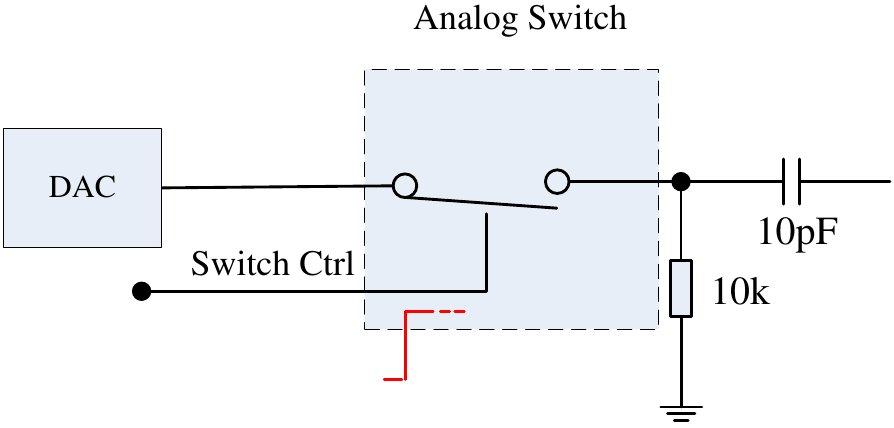
\includegraphics[width=0.7\linewidth]{chap/description/fig/fee_calibration}
\caption{电子学刻度电路原理}
\label{fig:ch2:fee_calibration}
\end{figure}


\subsection{温度/电流监测}
PSD的工作温度范围为\SI{-10}{\celsius}$\sim$\SI{30}{\celsius},探测器部件以及电子学器件的温度效应会对探测器的性能造成影响。
因此,PSD在探测器内部以及FEE板上多个位置放置了热敏电阻,对环境温度进行监测。
温度测量值最终通过FEE板上的ADC转化为数字量,并传输到载荷数管。
数据处理时,结合温度测量电路得到的环境温度值可以对温度效应进行修正。

空间中,单个带电粒子入射产生的瞬态电流触发CMOS器件中可控硅结构使其导通,由于可控硅的正反馈特性使电流不断增大,进入大电流再生状态,即导致锁定,这种现象被称为单粒子锁定(Single Event Latchup)。
单粒子锁定导致电流变大,局部温度升高;重新掉电、上电可以清除单粒子锁定,但如果没有迅速断电,过度的加热可能会造成器件的永久性损坏。
VA160是PSD最重要的功能器件,电流监测电路主要用于监测VA160是否发生单粒子锁定。
FEE采用电流采样电阻+ADC的方式监测VA160的-2.5V直流电源电压的电流,载荷数管会定时(1 次/秒)收集各FEE的电流值,如连续3次发现该电流值超标,载荷数管应立即把该FEE对应侧面的PMT高压降到低压档位,1秒钟后对DC-DC电源机箱发送相应断电指令,使该侧面的FEE关机,以保护FEE。


\section{机械支撑功能模块}
\label{sec:psd_support}
PSD所有的探测器功能模块、前端电子学功能模块和高压扇出板都安装在机械支撑结构当中。
PSD的机械结构能够稳固地支撑各内部组件,同时减缓火箭升空过程中的机械冲击和振动,保护脆弱部件不受损伤,保证PSD的功能完整性。

\begin{figure}[h!]
	\centering
	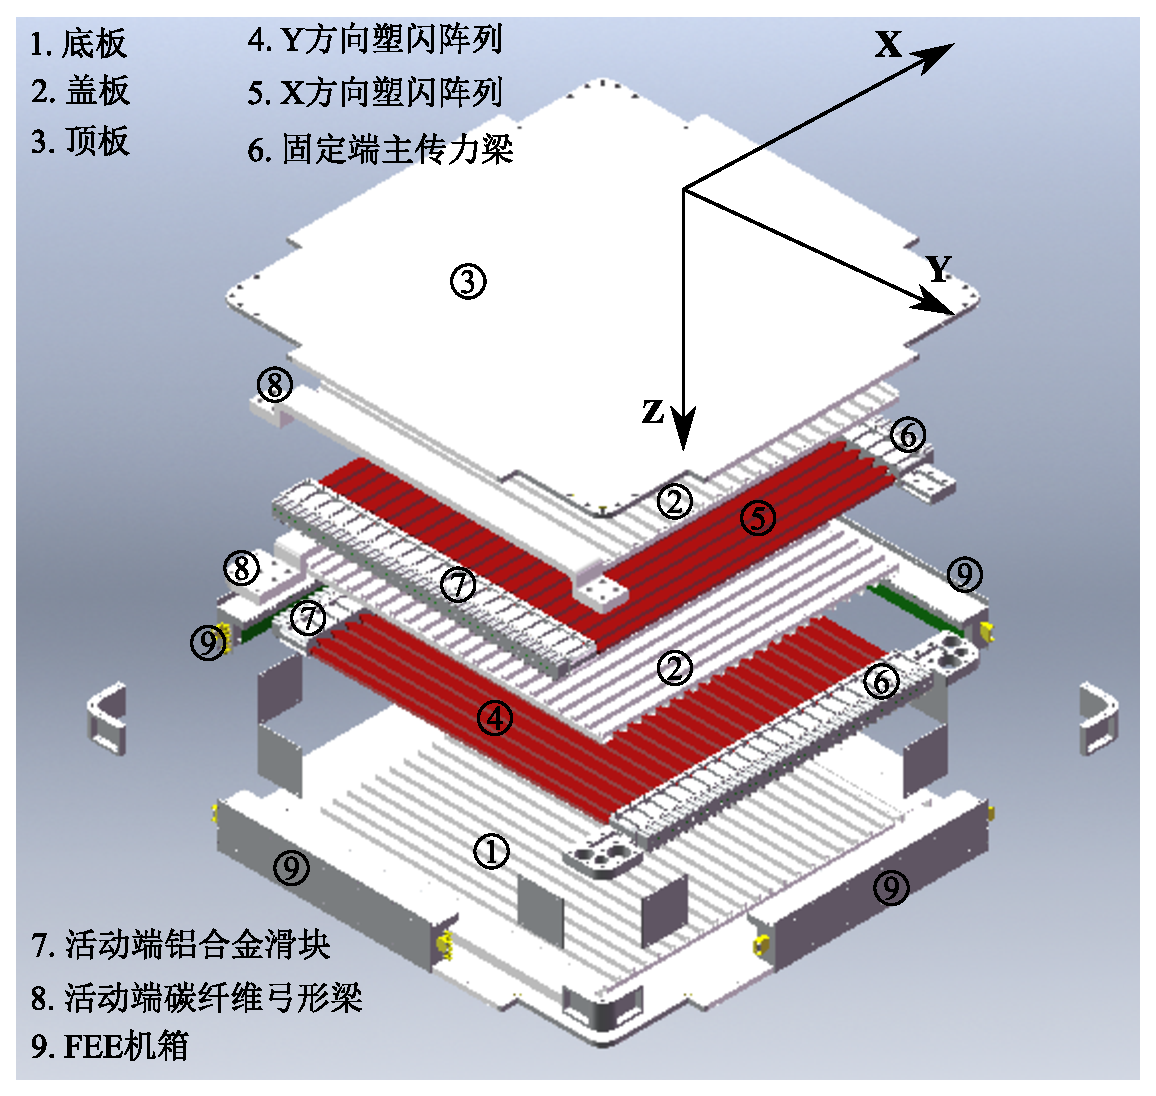
\includegraphics[width=0.8\linewidth]{chap/description/fig/psd_explosion.eps}
	\caption{PSD结构的爆炸图展示}
	\label{fig:ch2:psd_structure}
\end{figure}

图~\ref*{fig:ch2:psd_structure}给出了PSD整体结构的爆炸图展示。
底板和顶板,加上四个角上的连接法兰以及四个侧面的FEE机箱构成了PSD的主体包络($\SI{1200}{\milli\meter}\times\SI{1200}{\milli\meter}\times\SI{126}{\milli\meter}$)。
整个外包络组成一个封闭的内部空间,能够有效抵挡外部太阳光的照射,保护内部的PMT和塑闪单元条免受外部杂散光线的影响。
为了减轻重量和减少探测器灵敏面积内的物质量,底板和顶板采用碳纤维蒙皮的铝蜂窝板结构,并在四周主要承力部位预埋碳纤维方管和铝合金榫头组成的框架以加强刚度和强度。
连接法兰用于连接顶板和底板主传力结构,它采用铝合金材料。
FEE机箱内安装有该侧面对应的FEE前端电子学板、高压扇出板和信号转接板。
考虑到箱体结构的力学性能,FEE机箱的主体结构由铝合金整体铣制加工而成。
FEE机箱的侧板和顶板同样由铝合金材料加工而成,并与主箱体无缝衔接以提高电磁屏能力和导热性能。

PSD的主承力结构由4组梁结构和底板连接为一个整体组成,主要用于固定和保护塑闪单元条阵列及其PMT组件。
为便于结构装配,每根梁的主体由三层铝合金组件构成。
每组梁内部具有两排(一排21个,一排20个)“工”字形和圆柱形组成的凹槽结构,用于固定41个塑闪单元模块的一端。
“工”字形凹槽与塑闪单元条的“工”字形端头适配,用于固定塑闪单元条;圆柱形孔结构紧连“工”字形槽结构,用于安装PMT组件。
每两组梁结构固定一个塑闪阵列平面,并被分为固定端梁和活动端梁。
固定端梁只由三层铝合金组件组成,下层铝合金较其余两层稍长并直接与碳纤维底板连接,完全约束了单元条固定端的6个自由度。
活动端梁由三层铝合金组件和一个碳纤维弓形梁组成:三层铝合金组件自身连接成一个整体,该结构不和底板连接,也被称为铝合金滑块;碳纤维弓形梁与铝合金滑块外形完全适配并与底板直接连接,它和底板组成梁结构完全约束单元条活动端的5个自由度,底板和铝合金滑块间的摩擦力约束了沿塑闪单元条长度方向的自由度。
当温度变化时,塑闪单元条变形力能够克服摩擦力,并带动铝合金滑块小范围来回滑动从而释放塑闪单元条形变,保证单元条不因膨胀收缩而断裂。
碳纤维弓形梁对刚度和强度的要求都很高,因此选用高模量的碳纤维胶结而成。




	% 各章节
	\chapter{大动态范围读出方案的设计与验证}
\label{ch:large_dynmaicrange}
一个探测器本征的探测性能由其构型和使用的探测介质材料决定。
探测器的本征分辨是相对固定的,在研制阶段,一般通过物理过程的蒙卡模拟(如Geant4)对其进行研究。
探测器实际的探测性能还取决于其读出设计,包括读出器件的选择、读出方案以及前端电子学的设计。
探测器的读出设计相对灵活,往往需要针对探测器的功能需求进行特殊设计,在研制阶段,一般经过多次的‘设计-实验验证’循环来确定最佳的设计方案。
合理的读出设计可以将探测器的本征探测性能发挥到极致,这也是探测器研制的主要目标。

对于PSD来说,它首先需要覆盖质子数$Z=1 \sim 20$的重离子探测。
根据第二章的描述(见\ref{sec:description:psd_principle}节),相对论重离子在PSD塑闪单元条中的沉积能量近似正比于$Z^2$。因此,不同种类带电粒子在PSD中的输出信号幅度变化范围巨大,这对PSD探测单元模块读出方案的动态范围提出了上限要求。
另一方面,PSD同时需要对高能$\gamma$和高能$e$进行鉴别,即通过信号的有/无来判断入射粒子是否带电(见\ref{sec:description:psd_principle})。
为了降低$e/\gamma$误判率,PSD探测单元模块的读出方案需要足够敏感,能够有效区分带电粒子信号与电子学基线噪声信号,
这对其动态范围提出了下限要求。
一般的读出设计不能同时满足上述两方面的需求,我们需要对PSD探测单元模块的读出进行特殊设计,以满足其大动态范围的要求。

本章对PSD的读出方案设计进行了详细的论述,主要包括以下内容:PSD动态范围需求的估算,PSD读出方案的详细设计流程以及PSD大动态范围读出方案的实验验证。


\section{重离子在塑料闪烁体中的光产额}
\label{sec:dynamic_range:light_yield}
PSD使用PMT作为读出器件,因此入射粒子在塑料闪烁体中的闪烁光输出多少直接影响其输出信号的幅度。
在沉积能量密度不大的条件下,闪烁光输出与入射粒子的沉积能量大小成正比。
这种情况较为简单,我们可以通过对沉积能量大小的估算直接推出闪烁光输出的幅度范围。
但对于重离子来说,它们在物质中的沉积能量密度较大,此时猝灭效应\cite{birks_book_2013}(quenching effect)的影响显著。
因此,重离子引起的闪烁光输出与沉积能量大小不成正比关系,我们需要研究它们在塑料闪烁体中的光产额差异大小,为PSD动态范围需求的估算提供基础。

当带电粒子或$\gamma$射线入射到闪烁体内,使得闪烁体内的原子(分子)电离、激发,在退激过程中发光,这就是闪烁体发光的基本原理。
退激过程也可以不通过发射荧光光子的形式进行,而以其它形式将退激放出的能量转化为热能输出,这就是猝灭效应。
它使得闪烁体的发光量减少,并最终趋于饱和(saturation)。
猝灭效应与原初电离密度有关,电离密度越高,猝灭效应就越强,光响应偏离线性的程度也就越大。
闪烁体的猝灭效应一般用Birks定律进行描述\cite{birks_article_1951}:
\begin{equation}
	\frac{dL}{dx} = \frac{SdE/dx}{1+kBdE/dx}
	\label{eq:dynamic_range:birks_law_dE}
\end{equation}
其中$dL/dx$是单位路径的闪烁光产额,$dE/dx$是入射粒子的单位路径能量损失,$S$是发光效率(scintillation efficiency),$k$是猝灭因子,代表沉积能量中产生猝灭效应的比例,而$B$是一个常数。$kB$经常合在一起,被称为Birks系数。
当$dE/dx$较小时,猝灭效应并不明显,公式\ref{eq:dynamic_range:birks_law_dE}变为$dL/dx \approx AdE/dx$,即光产额与沉积能量成正比;当$dE/dx$很大时,公式\ref{eq:dynamic_range:birks_law_dE}变为$dL/dx \approx A/k_B$,即光产额近似是个常数,与沉积能量的大小无关,这就是猝灭效应导致的光饱和现象。
由于PSD只需对入射重离子的电荷量进行测量,我们希望得到塑闪光产额与入射粒子质子数$Z$(宇宙线重离子的核外电子都是完全剥离的,因此它们的电荷数就是质子数)的关系。
对于相对论重离子穿过薄的探测介质,$dE/dx \propto Z^2$。将这个关系带入到公式\ref{eq:dynamic_range:birks_law_dE},可到得到
\begin{equation}
	\frac{dL}{dx} = \frac{S' Z^2}{1+{k'}{B'} Z^2}
	\label{eq:dynamic_range:birks_law_Z}
\end{equation}
上式就是Birks定律应用到PSD中的结果。
在后面的论述中,我们都将使用$Z^2$来表述闪烁体光产额对入射粒子种类的依赖关系。

闪烁体的发光机制非常复杂,并没有统一的理论框架可以对其进行完备的描述。
公式\ref{eq:dynamic_range:birks_law_Z}只是一个半经验公式,其中的参数$S$和Birks系数虽然具有明确的物理意义,但一般需要通过对实验数据进行拟合得到。
而且,它们的具体数值与入射的粒子种类有关,这反应了猝灭效应的粒子种类关联性(particle-species dependence)。
另一方面,上述简单形式的Birks定律只能够描述闪烁体对低能入射粒子的光响应,当入射粒子能量升高到相对论能区时,就需要对Birks定律进行扩展。
相对论能区的光响应还有另外一个特点:那就是猝灭效应与入射粒子种类的关联性减弱,光产额主要取决于沉积能量大小\cite{matsufuji_response_1999}。
因此,Birks定律以及以下所有Birks定律的拓展形式中的自由参数具有普适性,即它们的值与入射粒子种类无关。

一种常见的扩展形式是在Birks定律的分母中加入$dE/dx$的二次项,即
\begin{equation}
	\frac{dL}{dx} = \frac{S' Z^2}{1+k'B'Z^2+C'Z^4}
	\label{eq:dynamic_range:birks_chou_law}
\end{equation}
其中$C'$是常数。这种扩展形式是Chou首次提出\cite{chou_nature_1952},因此上式被称为Birks-Chou公式。
另一种常见的扩展形式是基于闪烁体发光的BTV模型\cite{voltz_influence_1966,tarle_cosmic_1979}(Birks-Tarle-Voltz model,简称BTV模型)。该模型认为闪烁光按其产生的区域,可以被分为两部分“core”和“halo”两部分。
core区域在入射粒子的径迹附近,这里是电离过程发生的主要区域,分布有大量电离产生的低能电子;halo区域分布在core的外围,它由电离产生的少量高能$\delta$电子逃离core区域后形成。core区域内的电离密度较高,因此猝灭效应显著,该区域的光响应可以用Birks定律描述;halo区域的电离密度较低,猝灭效应可以忽略,该区域的光响应与沉积能量成正比。
假设halo区域的沉积能量占总沉积能量的比例为$F_s$,则基于BTV模型拓展的Birks定律可以表示为
\begin{equation}
	\frac{dL}{dx} = S(\frac{(1-F_s)Z^2}{1+B_s(1-F_s)Z^2}+F_sZ^2)
	\label{eq:dynamic_range:btv_law}
\end{equation}
其中$S$是一个常数,$B_s$表征猝灭效应强度的一个量。
除了这两种常见的扩展方式外,还有其它不较常使用的扩展形式,如Wright提出的\cite{wright_scintillation_1953}
\begin{equation}
	\frac{dL}{dx} = A \ln(1+aZ^2)
	\label{eq:dynamic_range:wright_law}
\end{equation}
其中$A$和$a$都是常数。
所有这些对Birks定律的扩展,它们的行为在$dE/dx$较小时都是一致的(即正比于光产额正比于沉积能量大小);但当$dE/dx$较大时,不同形式的扩展给出的结果相差很大。
虽然各种扩展形式在特定条件下,都可以准确地描述已有的实验数据点,但它们各有各的局限性,都不适合作为“第一性原理”来估算不同的相对论重离子在PSD塑闪条中的光产额差异。

\begin{figure}[htbp]
	\centering
	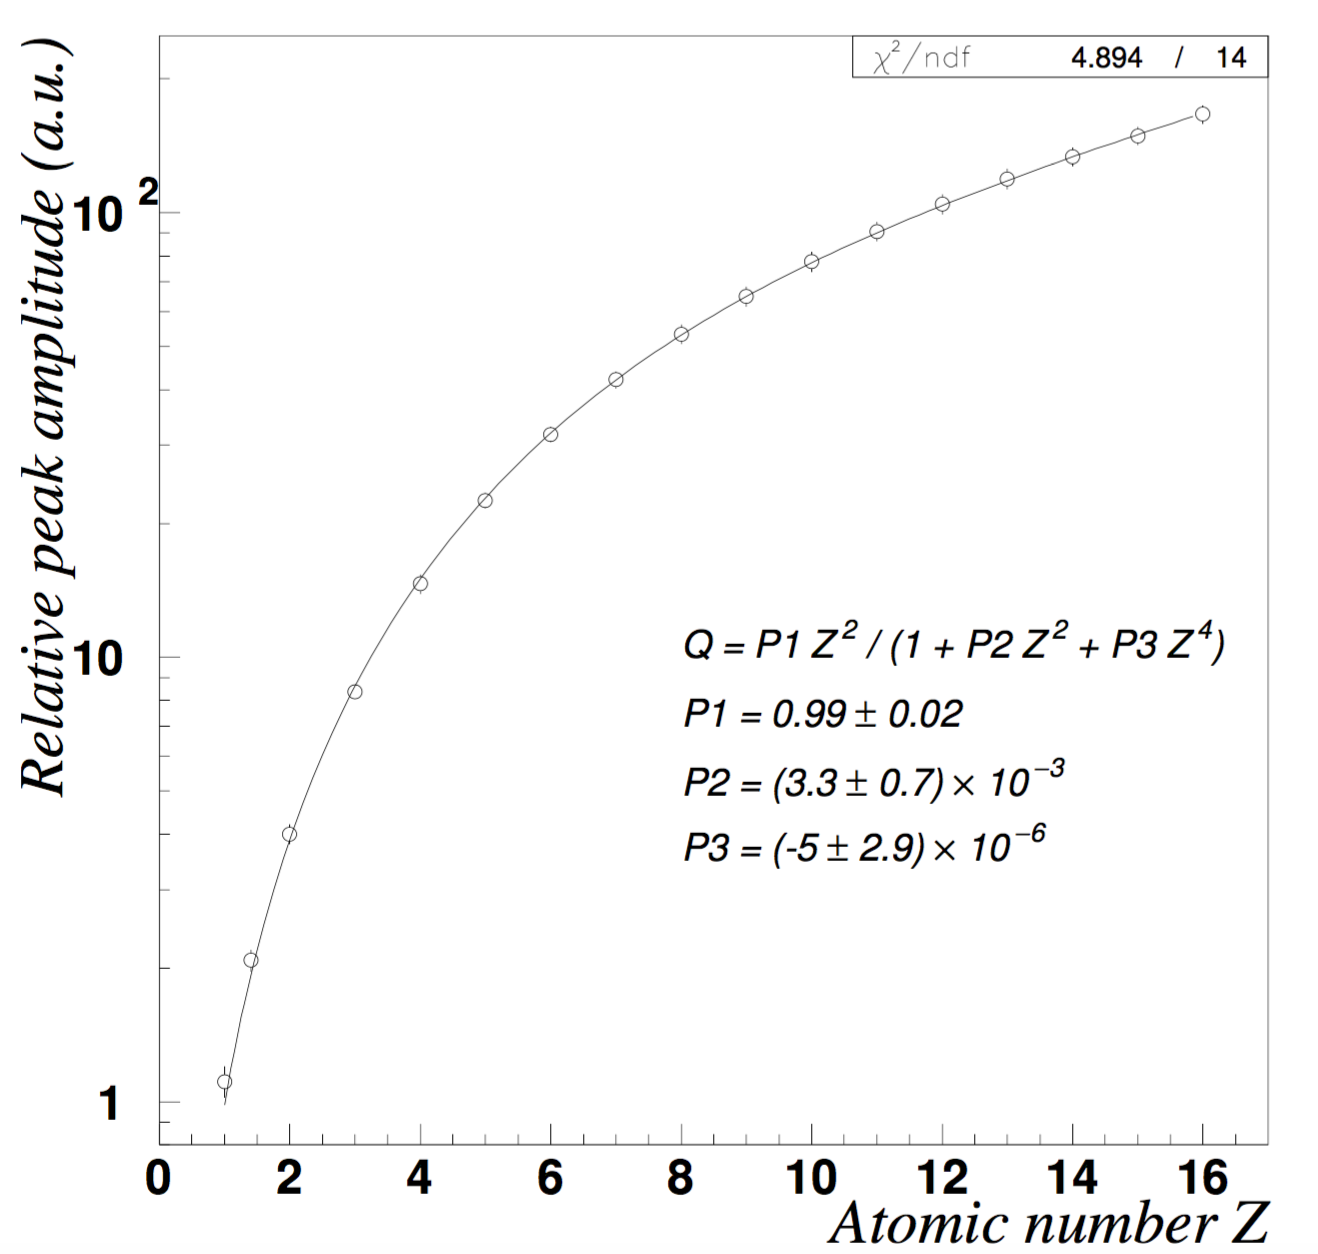
\includegraphics[width=0.6\textwidth]{chap/dynamic_range/fig/ams02_tof.png}
	\caption{AMS02-TOF得到的光响应曲线,横轴为质子数,纵轴为相对光产额。图中的圆点是实验数据点,实线是利用公式\ref{eq:dynamic_range:birks_chou_law}对数据点的拟合结果。}
	\label{fig:dynamic_range:AMS02}
\end{figure}

由于理论模型的局限性,我们基于AMS02-TOF束流测试的实验结果\cite{bindi_performance_2005}来得到相对论重离子在PSD塑闪条中的光产额差异。
束流测试在CERN的SPS进行,通过主束轰击Be靶得到不同种类的次级离子,主束使用的是\SI{20}{AGeV/c}和\SI{158}{AGeV/c}的Pb。
由于AMS02-TOF使用的探测介质与PSD完全一致,都是\SI{10}{mm}的EJ-200,该实验结果可以直接被PSD参考和使用。
图~\ref{fig:dynamic_range:AMS02}给出了AMS02-TOF得到的光响应曲线,数据点从$Z=1\sim16$。
使用扩展公式\ref{eq:dynamic_range:birks_chou_law}可以准确地拟合实验数据点,得到的拟合参数值为$S'=0.99(0.02)$,$k'B'=3.3(0.7)\times10^{-3}$,$C'=-5(2.9)\times10^{-6}$。
根据拟合结果,可以外推得到$Z=20$时的相对光产额,约为$Z=1$时的270倍。
该结果是我们估算PSD动态范围需求的基础。



\section{PSD动态范围需求的估算}
\label{sec:dynamic_range:estimation}
闪烁体的实际发光量不仅与其光响应有关,而且还与入射粒子穿过的厚度和能量涨落有关。
另外,PSD输出信号的大小直接决定于单元条端头PMT接收到的光子数,因此最终的动态范围还会受到光在单元条中传输导致的衰减效应的影响。
本节结合这些因素,对PSD的动态范围做了一个合理的估算,该估算结果被用于指导PSD探测单元模块大动态范围读出方案的设计。

在高能粒子探测器领域,设计人员经常使用最小电离粒子(Minimum Ionizing Particle,简称MIP)来对探测器进行测试和刻度。
对于PSD覆盖的相对论能区,所有的被测粒子(质子,重离子,电子)的能量都在Beth-Block曲线的费米坪区内,它们的电离能损与最小电离值相差不大,因此它们在本文中也可以被称为MIP粒子。
为了叙述的方便,我们将单电荷的最小电离粒子垂直穿过PSD塑闪单元条中心时端头PMT接收到的光输出量定义为\SI{1}{MIP},并以它为单位来表述PSD的动态范围需求。
由上节的结果可以看到,不同入射重离子在PSD塑闪条中的光产额最大相差270倍。
所有单电荷(singly charged)的MIP粒子在PSD单元条中都有相同的沉积能量,这也意味着它们有相同的光产额,因此上述结果可以拓展到所有带电粒子,即不同种类带电粒子在PSD塑闪单元条中的光产额为\SI{1}{MIP}$\sim$\SI{270}{MIPs}。

入射粒子在闪烁体中穿过的距离越大,它在物质中的能量沉积也就越大,产生的闪烁光子数也就越多。
对于PSD单元条这样厚度薄、密度小的探测介质,入射粒子在其中的单位路径能量损失率$dE/dx$以及单位路径的光产额$dL/dx$可以近似认为是个常数,这意味着能损大小以及光产额与入射粒子穿过的路径成正比。
DAMPE探测器设计有较大的视角,需要覆盖的入射角度为$[\SI{-60}{\degree},\SI{60}{\degree}]$。
这意味着入射粒子在PSD单元条中穿过的最长距离是垂直入射时的两倍。
因此,带电粒子在PSD中的光产额上限被扩展到\SI{540}{MIPs}。

上面讨论的都是平均光产额,而入射粒子在闪烁体中的能量损失过程和闪烁体的发光过程在本质上都是随机过程,这会带来光输出量的统计涨落。
实际的光输出量服从高斯分布,其中心值是平均光产额,标准偏差即探测介质的本征分辨率。
假设EJ-200的能量分辨率为\SI{10}{\percent},并且认为$5\sigma$可以覆盖整个高斯分布,则PSD单元条光产额的上限就扩展到\SI{675}{MIPs},而下限被减低到\SI{0.75}{MIPs}。

闪烁光子在入射粒子的击中位置处产生,它们需要在单元条内经过一系列的反射、折射和吸收过程,才能传输到端头,最终被PMT接收。
部分闪烁光子会在传输过程中损失掉,且传输的距离越长,损失的光子数越多。
为了尽量减少闪烁光长距离传输造成的衰减,PSD塑闪单元条进行了表面抛光,并且外部紧密包裹了一层高反射率的Tyvek纸以提高反射效率。
由于PSD单元条长度很长,上述措施并不能把光的传输衰减完全消除掉,这使得相同入射粒子在不同击中位置处产生的输出信号幅度并不一致。
该现象被称为光收集不均匀性,它极大地扩展了PSD输出信号的动态范围。
初步测试显示,从PSD单元条中心到单元条最远端的光衰减比例以及从单元条最近端到单元条中心的光衰减比例都可以被有效控制在\SI{50}{\percent}以上。
因此,PSD端头PMT接收到的闪烁光强度在应该在\SI{0.375}{MIPs}到\SI{1350}{MIPs}之间。

最后,为了将带电粒子产生的最小信号与电子学基线的噪声信号有效区分开来,同时适当预留部分动态范围供调节使用,PSD的动态范围需求被确定为$\SI{0.1}{MIPs}\sim\SI{1400}{MIPs}$。

\section{大动态范围读出方案的设计}
\label{sec:dynamic_range:design}

\subsection{设计思路}
\label{sec:dynamic_range:readout_scheme}
PSD使用ASIC芯片VA160进行电荷测量。该芯片集成了32个输入通道,每个通道的动态范围为$\SI{-3}{\pico\coulomb}\sim\SI{13}{\pico\coulomb}$(详见第\ref{ch:description}章)。显然,单个VA160通道不能够覆盖所需的动态范围。因此,PSD探测单元模块采用了下述的读出设计:以双打拿极引出的方式,从单个PMT得到两路不同增益的输出信号,然后将两路信号分别输入到不同的VA160的测量通道中。当光输出量较小时,可以使用低增益的通道进行测量;当光输出量较大时,此时低增益通道已经饱和,可以使用高增益的通道进行测量。同时,为了降低高增益通道对低增益通道的干扰,高增益通道的信号和低增益通道的信号被输出到不同的VA160芯片中,如图~\ref{fig:dynamic_range:readout_scheme}所示。

\begin{figure}[!htb]
	\centering
	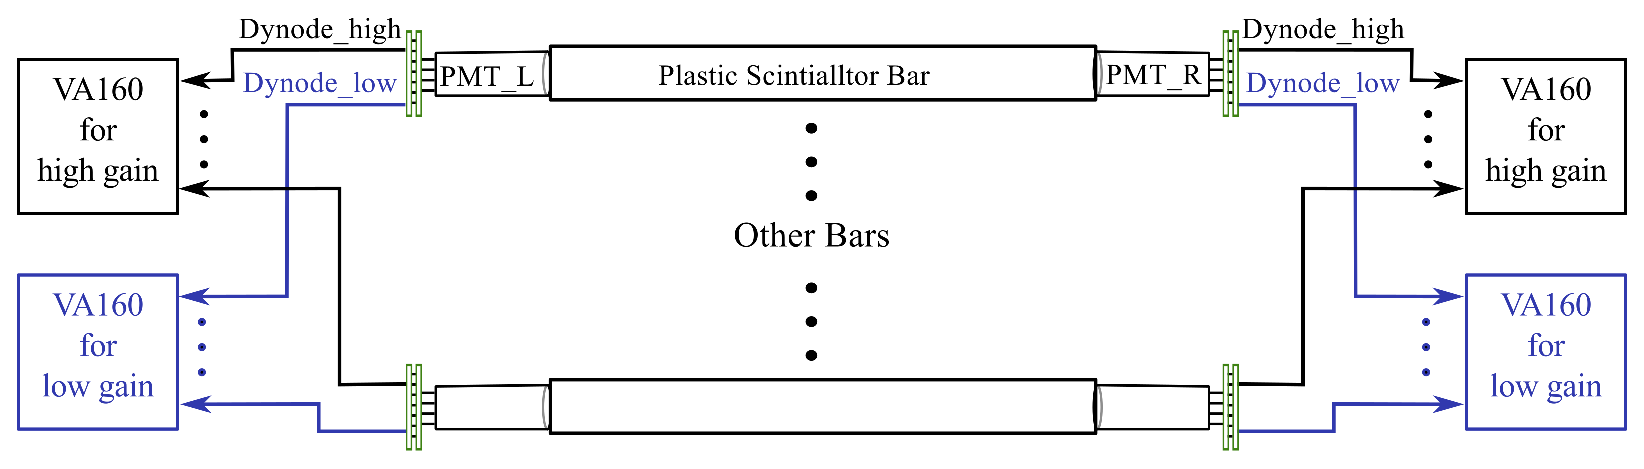
\includegraphics[width=\textwidth]{chap/dynamic_range/fig/readout_scheme.eps}
	\caption{PSD探测单元模块的读出方案}
	\label{fig:dynamic_range:readout_scheme}
\end{figure}

中国科学院近代物理研究所基于VA160芯片开发了PSD的前端电子学模块(Front-End Electronic,简称FEE),详见第\ref{ch:description}章。
测试显示,该FEE模块的有效线性范围为$\SI{0}{\pico\coulomb}\sim\SI{12}{\pico\coulomb}$,且每个测量通道的电子学噪声可以控制在\SI{6}{\femto\coulomb}内~\ref{fig:dynamic_range:fee_test}。
假设最少需要$5\sigma$的分离度来区分真实信号与基线噪声,这意味着PSD读出电子学对\SI{0.1}{MIPs}的测量值应该大于\SI{30}{\femto\coulomb},即$\SI{1}{MIP} \ge \SI{300}{\femto\coulomb}$。
因此,高增益打拿级对应通道的动态范围应该覆盖$\SI{0.1}{MIPs}\sim\SI{40}{MIPs}$余下的动态范围由低增益打拿级对应的通道覆盖,这限制了两个打拿级间的增益系数必须$\ge 35$。
这两个要求是下一节中对打拿极进行选择的依据。

\begin{figure}[!htb]
\centering
\subfloat[][FEE某通道的基线噪声谱]{
	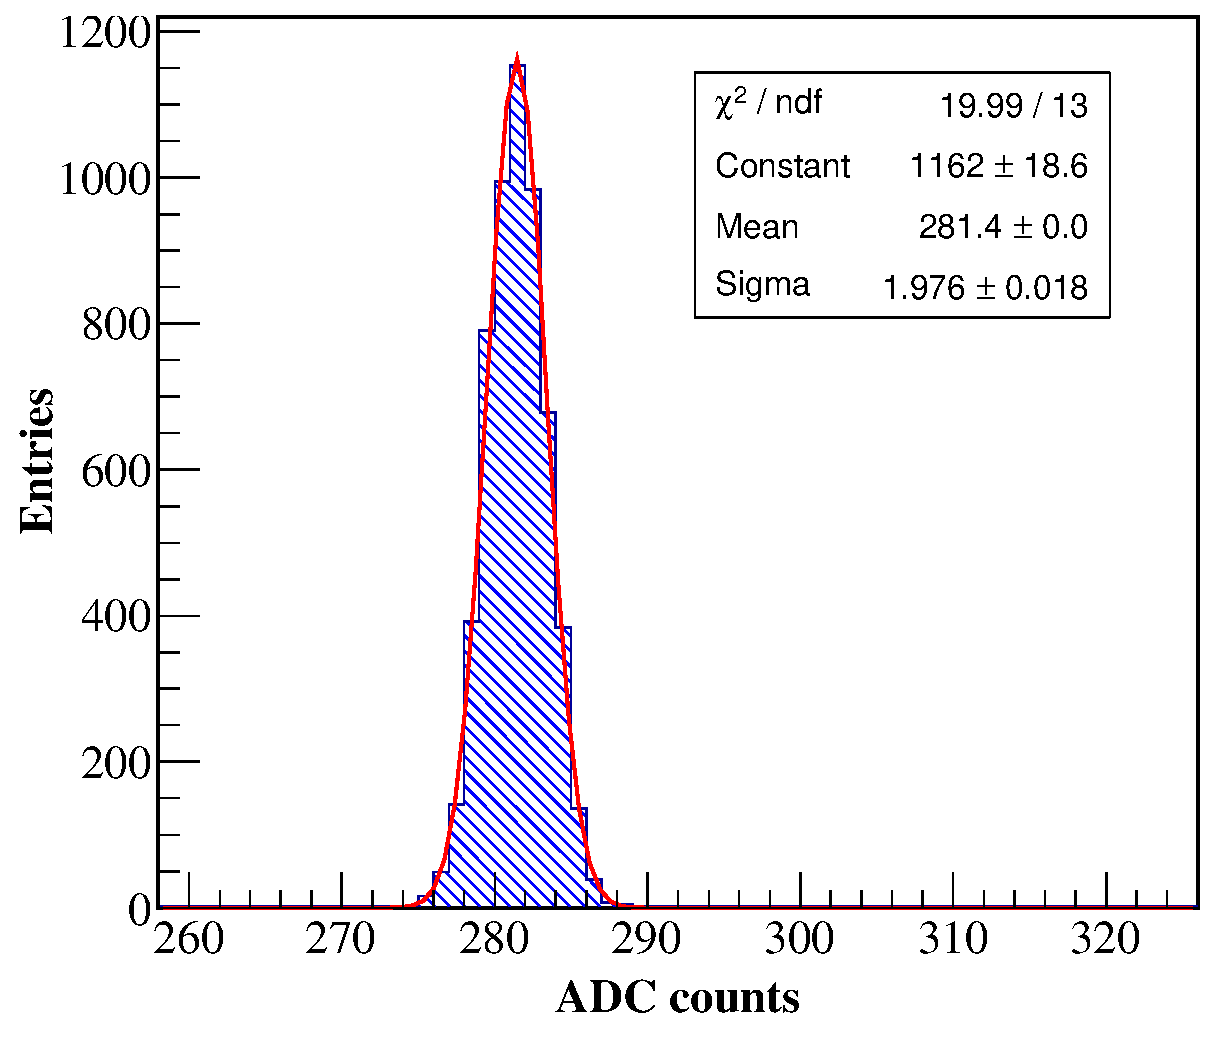
\includegraphics[width=0.48\textwidth]{chap/dynamic_range/fig/ped.eps}
}
% \hfill
\subfloat[][FEE某通道的电子学刻度结果]{
	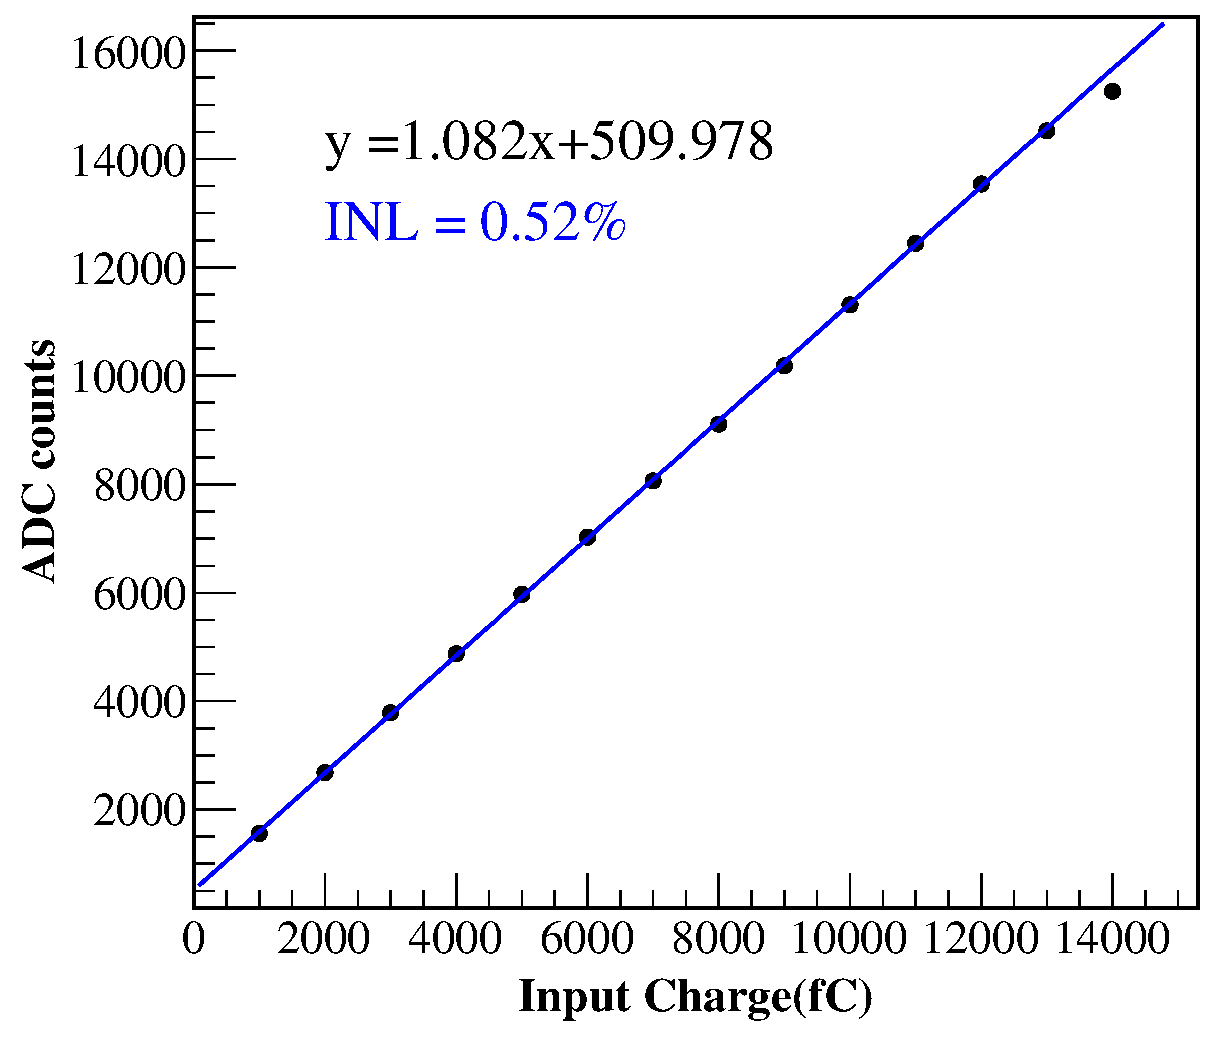
\includegraphics[width=0.48\textwidth]{chap/dynamic_range/fig/elec_calib.eps}
}
\label{fig:dynamic_range:fee_test}
\caption{FEE的测试结果}
\end{figure}

\subsection{打拿极的选择}
\label{sec:dynamic_range:dynode_selection}
PMT的不同打拿极对应不同的增益系数,而R4443具有10个打拿极级数。
为了从中选出合适的两个打拿极级数用于信号引出,需要对\SI{1}{MIP}信号产生的平均光电子数(Photoelectrons,简称PE)进行估算(这里的\SI{1}{MIP}同\ref{sec:dynamic_range:estimation}节的定义,即需要对单电荷最小电离粒子垂直穿过PSD塑闪单元条时端头PMT产生的光电子数进行估算)。
根据得到的平均光电子数值,就能进一步估算出各个打拿极输出信号的电荷量。
最终,结合上一节得到的动态范围要求和打拿极间的相对增益要求,我们就能确定合适的打拿极级数。

单电荷最小电离粒子在\SI{10}{mm}塑料闪烁体材料中的沉积能量约为\SI{2}{MeV},而EJ-200的发光效率约为$\SI{e4}{photons/MeV}$(见表~\ref{tab:description:ej200})。
产生的闪烁光子在空间中的分布是各向同性的,因此各有一半光子指向单元条的两端。
这些光子首先在单元条的表面经历一次折射过程,出射角度小于全反射角的光子会直接逃逸出单元条内部,只有出射角度大于全反射角的那些光子才有可能在单元条内部经过多次反射并最终传输到单元条端头。
根据EJ-200的折射率(见表~\ref{tab:description:ej200})可以计算得到,这部分光子只占总光子数的\SI{22.5}{\percent}。
部分光子在单元条内部的传输过程中会被吸收,这就是光衰减效应,它由塑闪单元条的光衰减系数决定。
到达端头的光子穿过单元条端面进入耦合介质EJ-560,然后被传输到PMT的端面,最终击中光阴极并通过光电效应产生光电子。
结合所有这些因素,可以将\SI{1}{MIP}产生的平均光电子数估算为
\begin{align}
 N_{PEs} &= \frac{1}{2} \times \SI[per-mode=symbol]{2}{\mega\electronvolt} \times \SI{e4}{\per\mega\electronvolt} \times 0.225
           \times \varepsilon_{1} \times \varepsilon_{2} \times \varepsilon_{3} \times \varepsilon_{4} \nonumber \\
         &\approx \SI{48}{PEs\per{MIP}}
\label{eq:dynamic_range:pe_estimation}
\end{align}
其中,$\varepsilon_1$ ($\approx$0.5)是从单元条中心到端头的光传输衰减率;$\varepsilon_2$ ($\approx$0.3)是几何因子,它由R4443入射窗和PSD单元条端面的有效耦合面积决定;$\varepsilon_3$ ($\approx$0.95)是耦合介质EJ-560的传输效率;而$\varepsilon_4$ ($\approx$0.15)是R4443光阴极的量子效率(quantum efficiency),它是表示光电转换的效率,是出射光电子数与入射光子数的比值。

根据表~\ref{tab:description:r4443},在标称工作电压下并使用标准分压器(即所有打拿极间具有相同的电压降)的条件下,R4443阳极增益$G$的典型值为\SI{1e6}{}。
R4443的所有打拿极使用相同的材料,因此它们的二次发射系数$\delta_i$是相等的;另外,在极间电压足够大的情况下,打拿极间的传输效率$\eta_i$近似为\SI{100}{\percent}。
因此,可以认为所有打拿极的极间增益系数$g_i=\delta_i\eta_i$也是相等的。
于是,根据公式\ref{eq:dynamic_range:gain}可以得到:在标准工作电压下,极间增益$g$约为3.98。
\begin{equation}
	G = \prod_{i=1}^{n} g_i = g^n
	\label{eq:dynamic_range:gain}
\end{equation}

\begin{figure}[!htb]
	\centering
	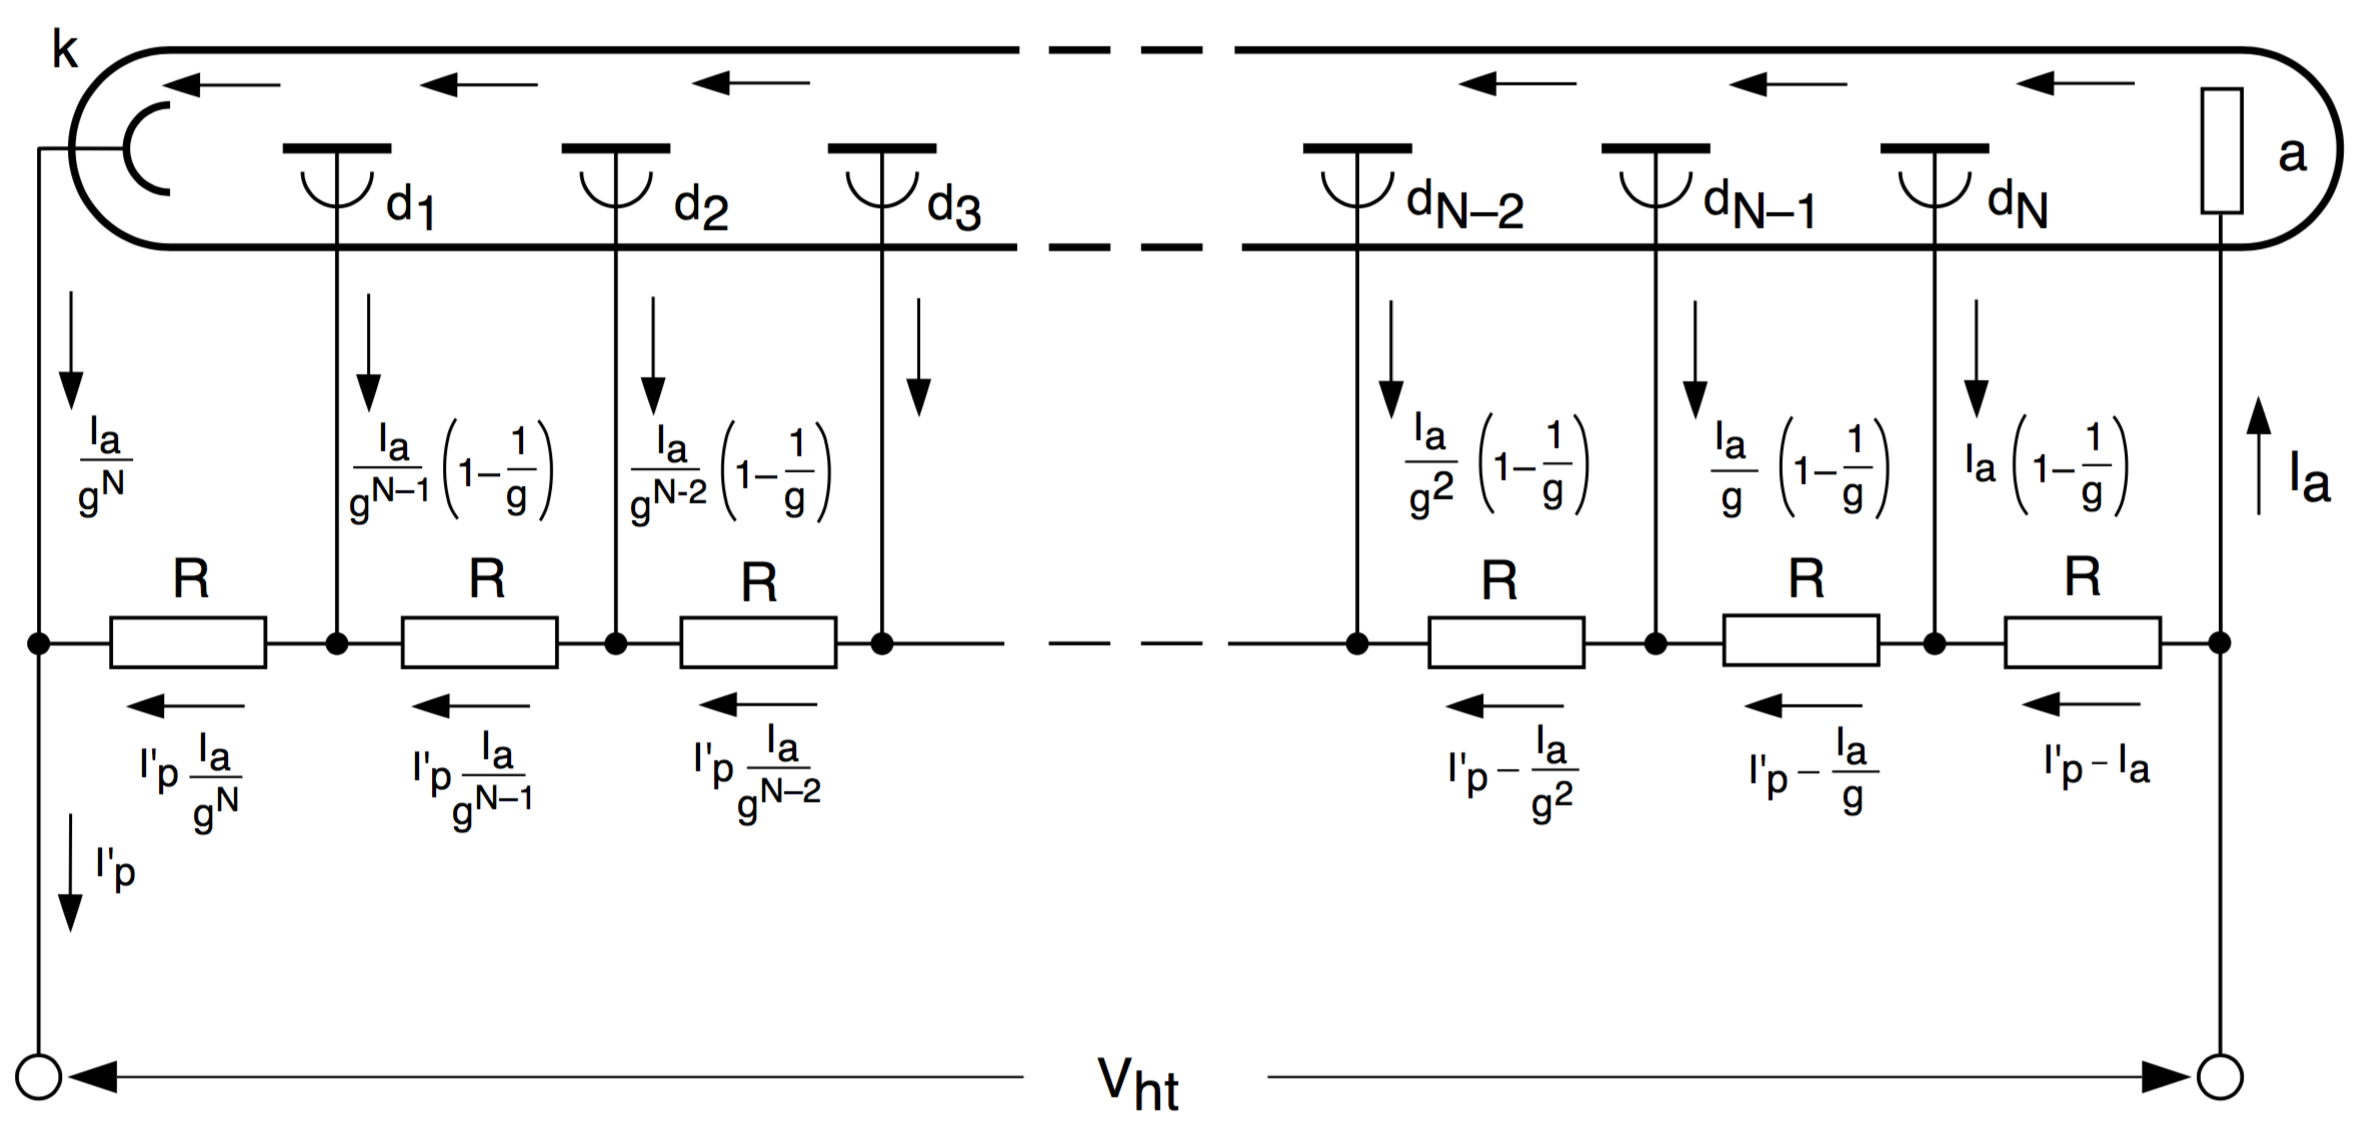
\includegraphics[width=0.9\textwidth]{chap/dynamic_range/fig/pmt_current_distribution_photonics.png}
	\caption{Caption here}
	\label{fig:figure1}
\end{figure}

\subsection{分压器电路的设计}
\label{sec:dynamic_range:hv_divider}

\begin{figure}[!htbp]
	\centering
	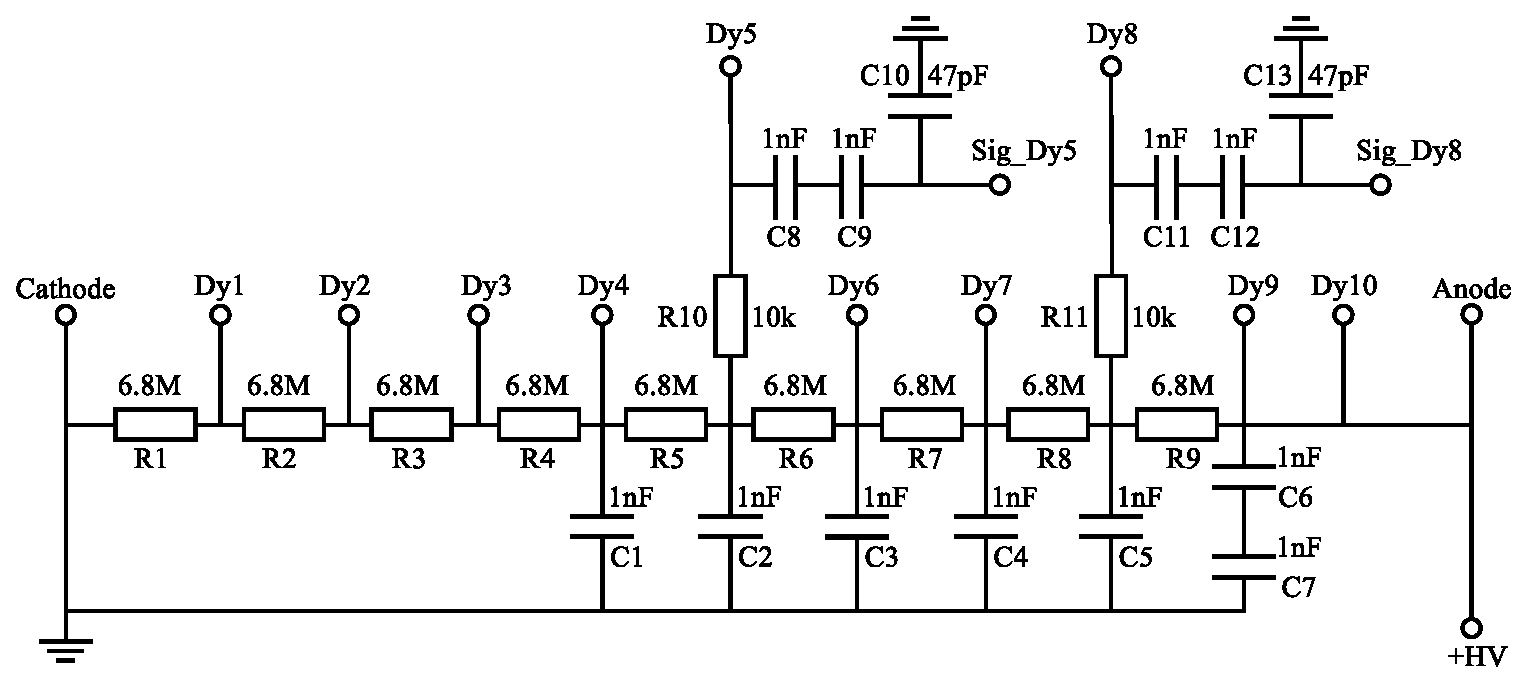
\includegraphics[width=0.95\textwidth]{chap/dynamic_range/fig/divider.eps}
	\caption{PSD的分压器电路原理图}
	\label{fig:dynamic_range:divider}
\end{figure}

\section{大动态范围读出方案的原理验证}
\label{sec:dynamic_range:verification}

% \subsection{LED的测试}
% \label{sec:dynamic_range:led}

\subsection{宇宙线的测试}
\label{sec:dynamic_range:cosmic_ray}

\begin{figure}[!htbp]
	\centering
	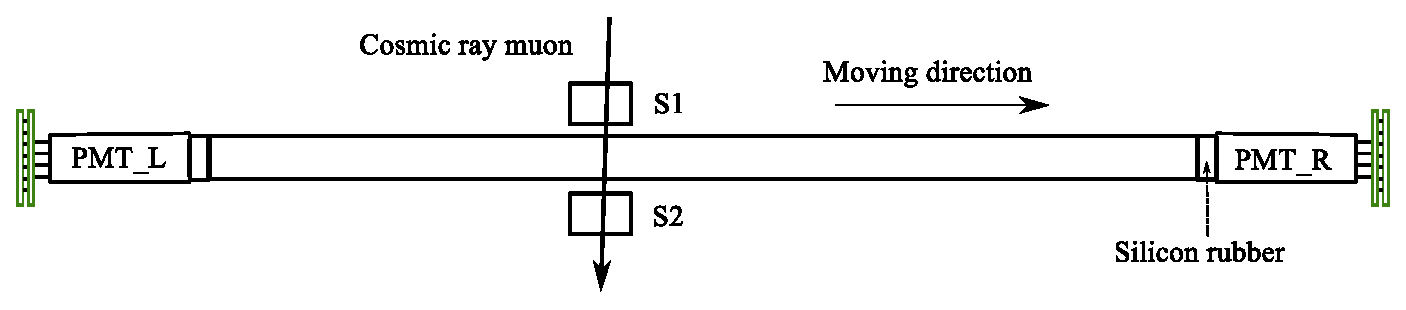
\includegraphics[width=0.95\textwidth]{chap/dynamic_range/fig/cosmic_test.eps}
	\caption{PSD探测单元模块的宇宙线测试}
	\label{fig:dynamic_range:cosmic_test}
\end{figure}

\begin{figure}[!htbp]
	\centering
	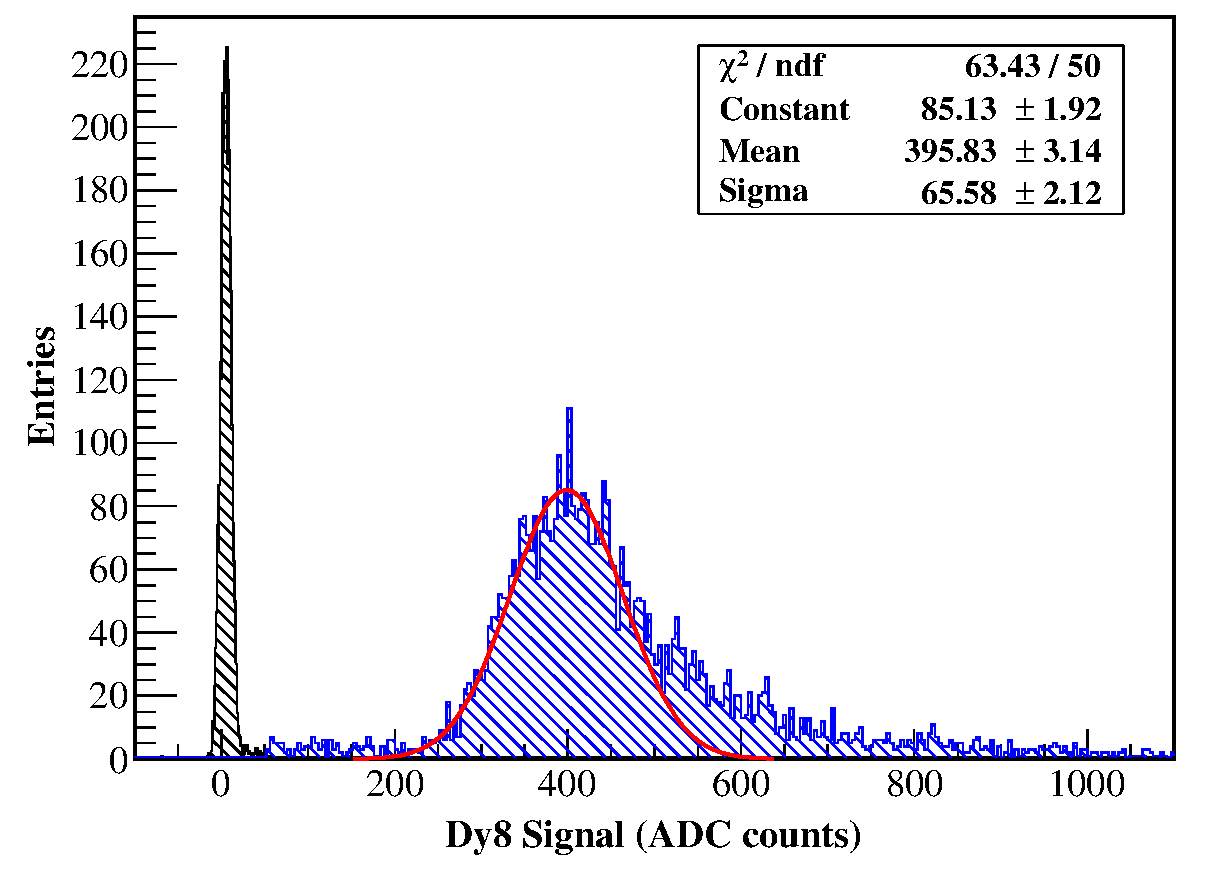
\includegraphics[width=0.6\textwidth]{chap/dynamic_range/fig/mip.eps}
	\caption{PSD单元条中间位置处的MIP响应}
	\label{fig:dynamic_range:mip}
\end{figure}

\begin{figure}[!htbp]
	\centering
	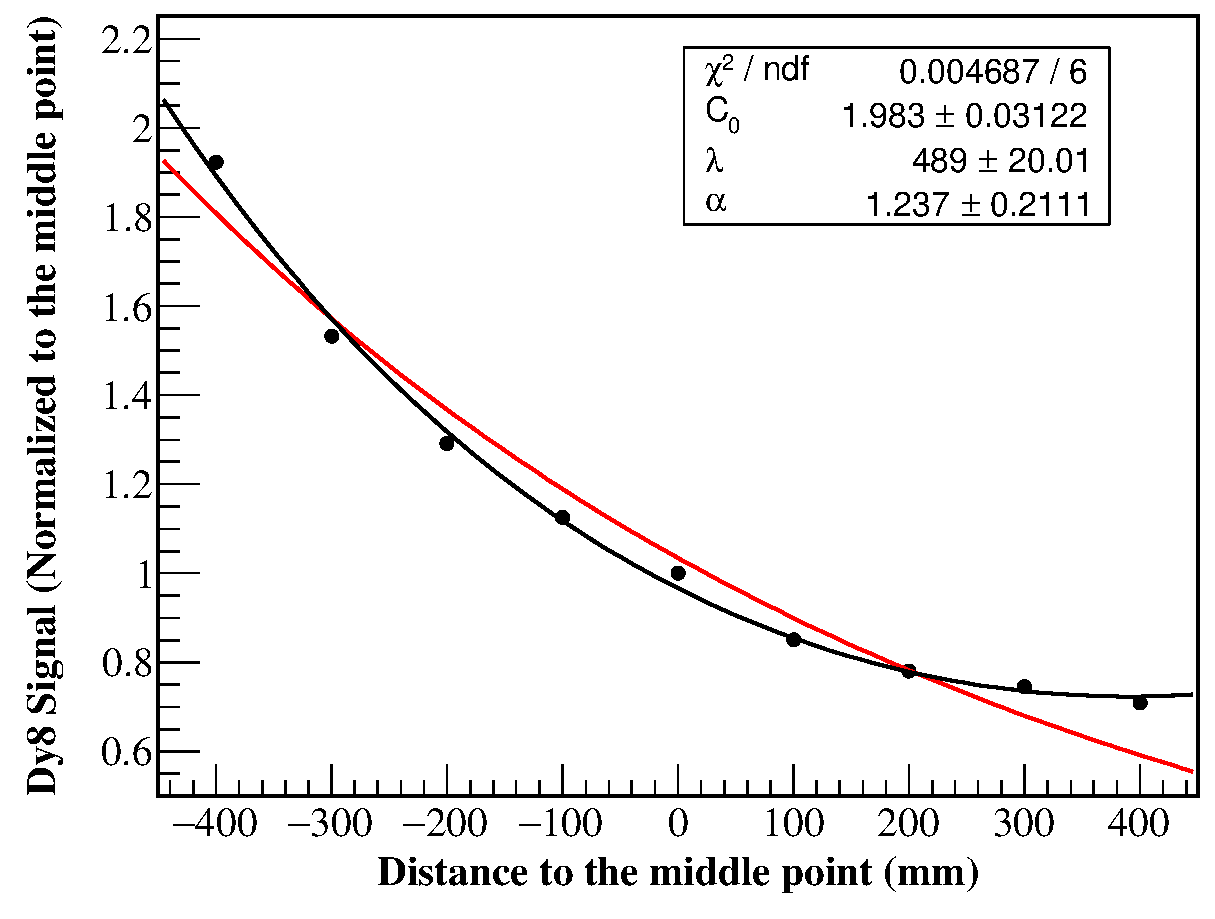
\includegraphics[width=0.6\textwidth]{chap/dynamic_range/fig/atten_right.eps}
	\caption{PSD单元条的光衰减曲线}
	\label{fig:dynamic_range:attenuation}
\end{figure}

\begin{figure}[!htbp]
	\centering
	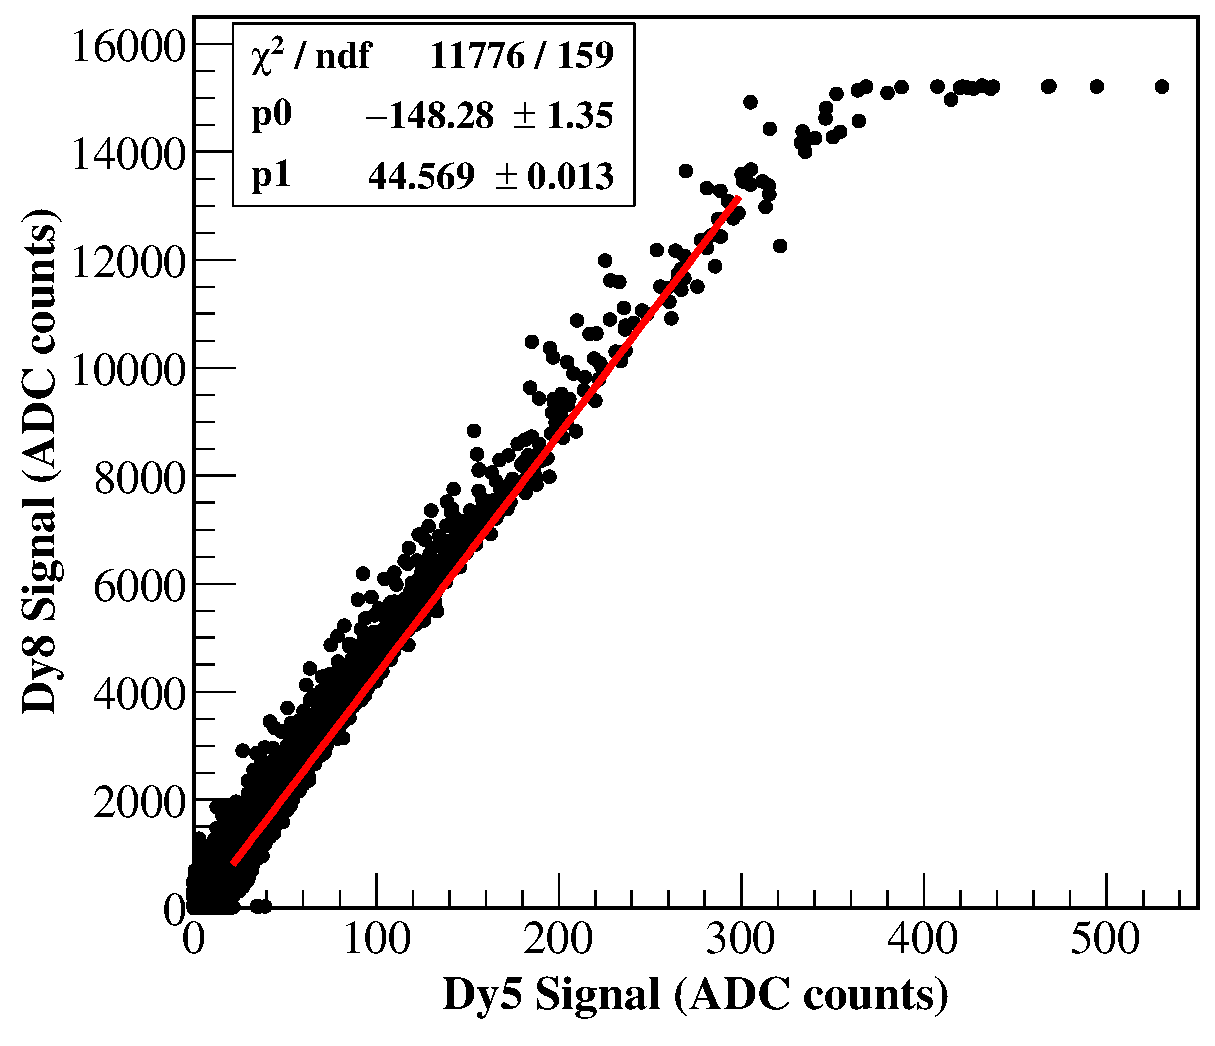
\includegraphics[width=0.6\textwidth]{chap/dynamic_range/fig/dy58.eps}
	\caption{Dy8与Dy5通道的ADC道数关联谱}
	\label{fig:dynamic_range:dy58}
\end{figure}

\subsection{中能轻核束流的测试}
\label{sec:dynamic_range:ion_beam}

\begin{figure}[!htbp]
	\centering
	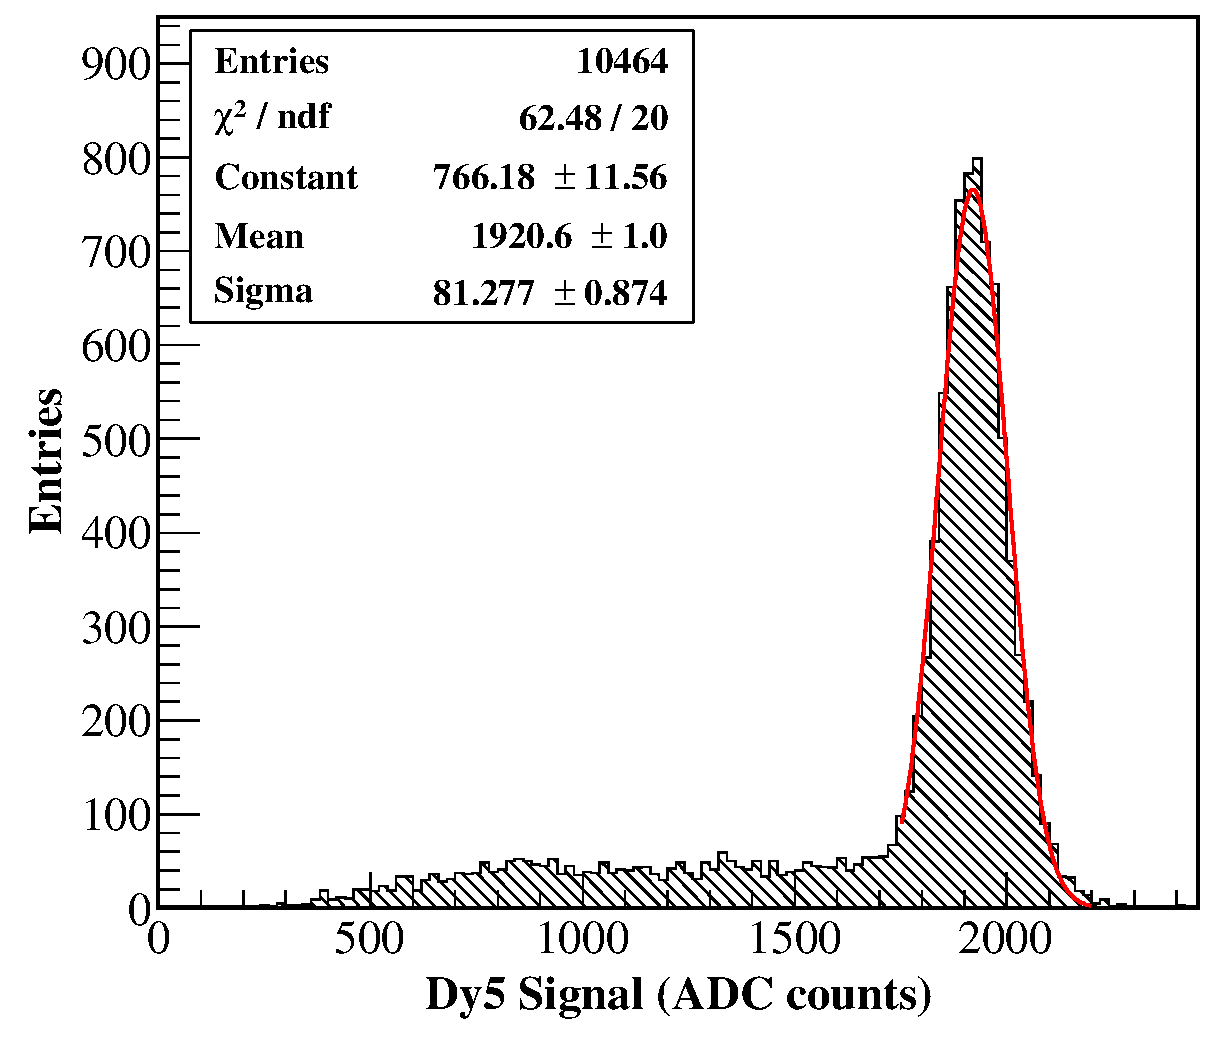
\includegraphics[width=0.6\textwidth]{chap/dynamic_range/fig/Ar.eps}
	\caption{$^{40}Ar$击中PSD单元条中间位置处的ADC原始谱}
	\label{fig:dynamic_range:Ar}
\end{figure}
	% 各章节。
	\chapter{光电倍增管的性能测试与筛选}
\label{ch:pmt_test}
由于制造工艺的限制,光电倍增管具有很强的个体差异性,即不同管子的性能差异较大。
因此,在光电倍增管大规模应用时,往往要求对每支管子进行详细的测试,以得到它们各自的性能参数信息。
利用这些信息,探测器的研制者可以淘汰性能参数不达标的管子,可以决定管子在探测器整体中的安装位置,可以得到管子的额定工作电压,甚至可以在探测器部署运行后调节其实际工作电压,最终使探测器整体的探测性能达到最佳。

对于PSD所使用的R4443型光电倍增管,Hamamatsu公司对每支出厂的管子进行了基本的性能测试(包括阳极暗电流、长时间稳定性、阴极/阳极的光灵敏度以及阴极/阳极的蓝光灵敏度),并提供了相应的测试结果。
然而,这些测试只在一个工作电压点进行,而且使用的测试条件(连续、强烈的白炽光照射)与R4443在PSD中的实际工作条件(低强度、低频率的脉冲光照射)迥异。
另外,PSD使用双打拿极引出的分压器电路与上述出厂测试使用的标准分压器差别较大,导致R4443的工作状态也不一致。
因此,这些参数信息只能定性地给出各支管子的基本性能,不能作为PSD研制过程的定量参考。

上述因素决定了:需要根据PSD的具体需求,在实验室独立对R4443光电倍增管进行性能参数测试。
为此,我们专门设计并搭建了一套的PMT批量测试平台。
本章对该测试平台进行了介绍,并详细叙述了该平台在R4443光电倍增管的性能测试中的应用以及测试结果。
根据测得的性能参数数据,依据性能最佳的原则,我们进一步对所有管子进行了筛选,选出了可以用于PSD安装的光电倍增管。

\section{PSD对光电倍增管的测试需求}
由于PSD没有参加DAMPE的触发系统,PSD不需要对粒子的入射时间进行测量。
因此,R4443的时间性能参数没有实际的参考价值,无需在实验室对其进行专门的测试。
另一方面,PSD通过测量沉积能量来实现其所有功能(见第\ref{sec:description:psd_principle}节),而光电倍增管的增益是直接影响探测器能量响应的重要参数。
因此,我们的测试主要关注R4443与增益相关的性能参数,这包括Dy8的增益以及Dy5和Dy8间的相对增益(简称Dy58比值)这两个方面。

PSD要求各探测单元模块的能量响应均匀性好于\SI{25}{\percent}。这意味着,需要

高压分组的限制

\section{PMT批量测试平台}
\label{sec:pmt_test:testbench}
PSD的研制过程中涉及大量的PMT测试工作,包括对570支R4443裸光电倍增管的细致性能测试以及在PSD建造过程中将近200个PMT组件的质量测试(详见第\ref{ch:construction}章)。
为了提高工作效率,减轻测试人员的工作负担,我们设计并建造了能够用于PMT大批量测试的专用测试平台。

\subsection{功能与特点}
\label{sec:pmt_test:testbench_functions}
PMT的批量测试是在大型探测器研制过程中经常碰到的工作。
因此,该测试平台虽然是为了DAMPE-PSD项目专门研制的,但我们在设计中充分考虑了该平台的拓展性和可移植性,使得它能够方便地应用于其它项目的PMT测试工作。
该测试平台的主要特点可以归结为如下几点:
\begin{enumerate}
	\item 测试容量大。大型探测器项目动辄涉及成百上千支PMT的测试,如果能够对多支PMT同时进行测试,就可以显著提高工作效率,加快项目进程。该测试平台最大测试容量达到25支PMT,满足大部分项目的测试需求。
	\item 自动化程度高。PMT的细致测试往往涉及不同的性能指标,一次完整的测试需要花费几个小时的时间。这个过程中,需要对大量的仪器设备进行重复操作,如升降高压、切换光强度、移动PMT位置等等。此时,人工操作不仅效率低,而且是不可靠的。因此,该测试平台的关键组件都是用了程控设备,并开发了相应的控制软件,实现了常用设备操的自动化。这样,在PMT的整个测试过程中,人工干预只存在于PMT的安装与卸载,以及相关软件的配置,提高了测试工作的可靠性。
	\item 功能完备。该测试平台能够满足很多潜在的测试需求,即便有些在PSD的研制过程中并不需要。因此,平台使用了一些特殊的硬件模块以及通用的仪器设备。尤其是,我们将三维移动性作为该平台的一个基本功能,使得平台可以用于PMT光阴极的位置扫描。
	\item 扩展性强。测试平台采用模块化设计,其硬件平台是可扩展的,各硬件模块之间的耦合相对松散。这方便了硬件的更换或升级,并可以实现较为复杂的测试方案。软件框架同样基于模块化设计,并对底层硬件进行了虚拟化,使得顶层的测试功能不因底层硬件的改动而有大的变动,增强了测试程序的可移植性。
\end{enumerate}

图\ref{fig:pmt_test:testbench_schematic}给出了PMT批量测试平台的原理框图。
该平台最多可以同时对25支PMT进行测试。光脉冲由一个蓝光LED产生,它经过积分球和集束光纤组成的光分配系统被分成25份,被分别传输到待测PMT的入射端面。
待测PMT都安置在一个固定平台上,而光源和光分配系统被固定在一个三维移动平台上。两个平台相对摆放,从而实现了对所有待测PMT的光阴极位置扫描。
固定平台上同时安置有两支监控PMT,也接受来自光分配系统的两路入射光脉冲。
在整个测试周期中,两支PMT的位置相对于入射光纤固定不变,因此它们被用于监控LED光源以及整个测试平台性能的稳定性。
这两个支撑平台以及上面的所有测试设备都被放置在一个大小为$176cm\times100cm\times78cm$的铝合金暗箱中(见图\ref{fig:pmt_test:blackbox}),箱子的内壁用黑色图层覆盖以降低内部的杂散光污染。

\begin{figure}[htb]
	\centering
	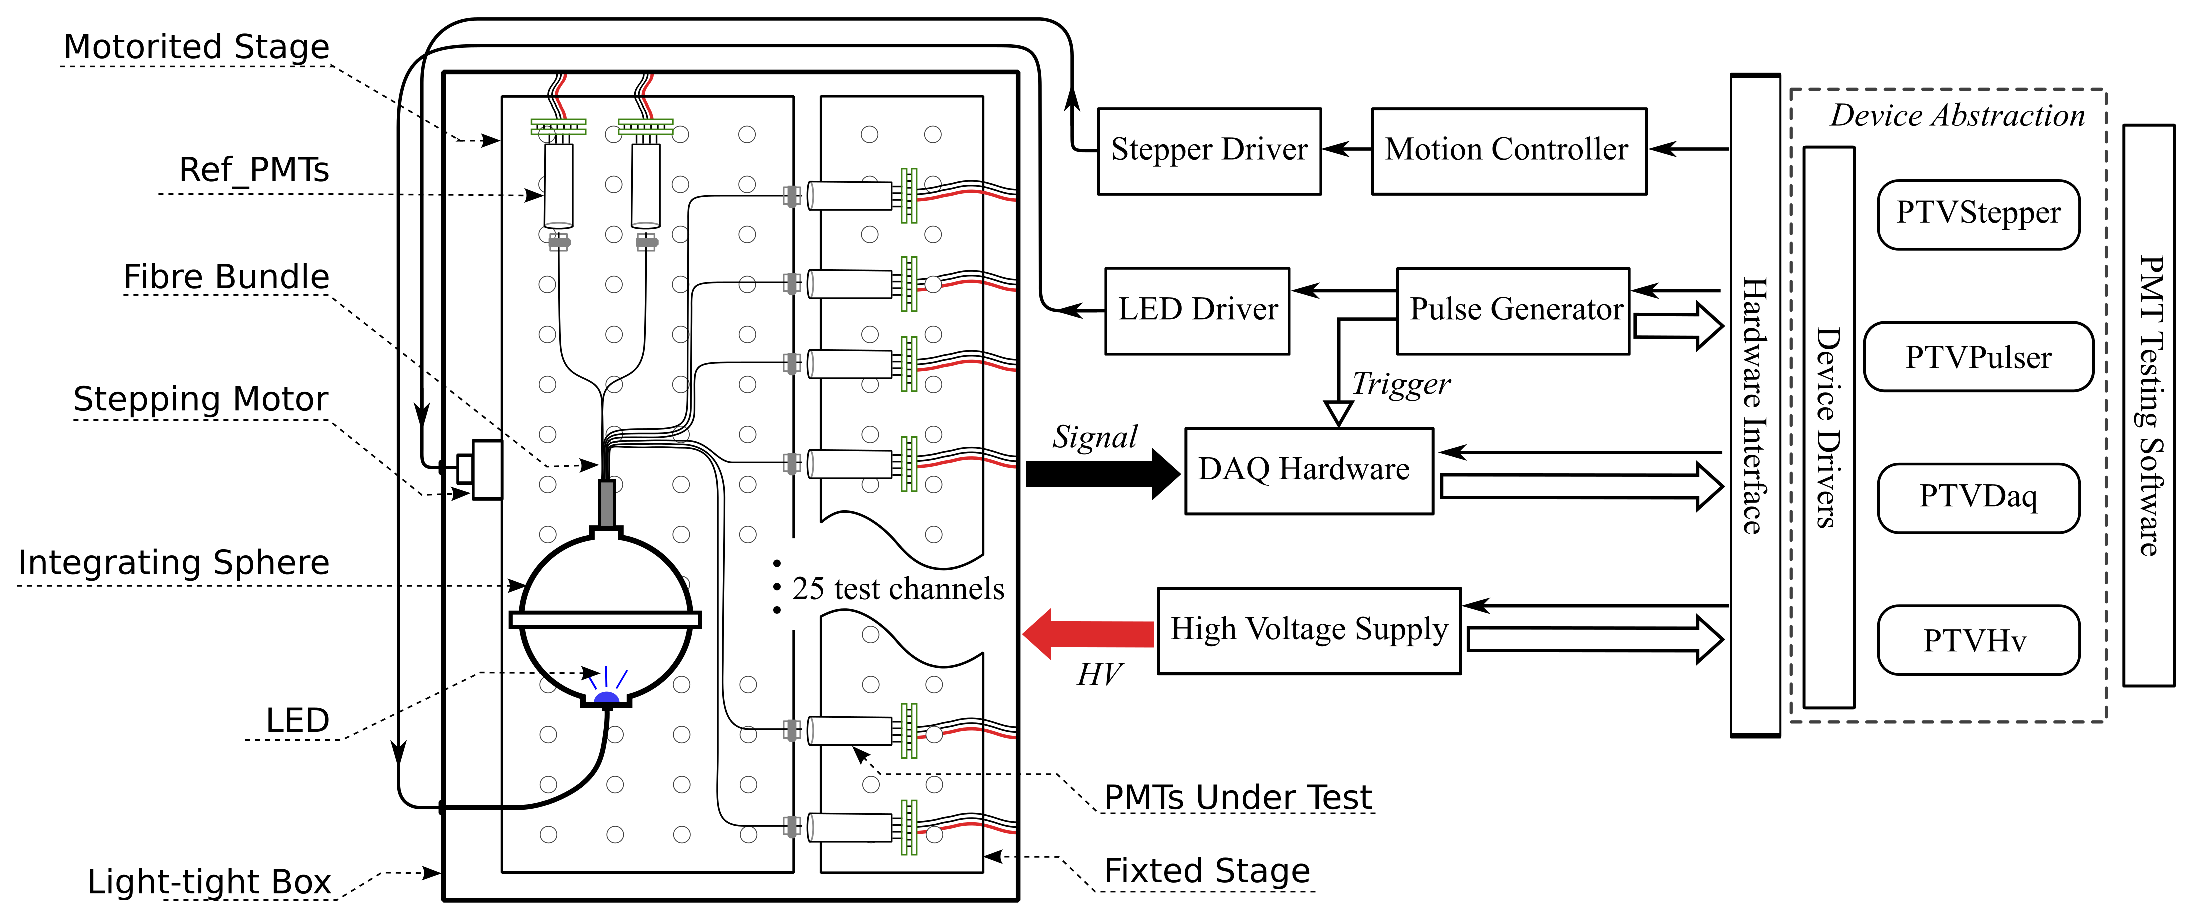
\includegraphics[width=\textwidth]{chap/pmt_test/fig/testbench_schematic.eps}
	\caption{PMT批量测试平台的原理框图}
	\label{fig:pmt_test:testbench_schematic}
\end{figure}

PMT测试平台的大部分辅助设备被都放置在铝合金暗箱的外围,它们与内部器件的连接线缆穿过箱子上不透光的通孔相互联接。
这些辅助设备可以被分为四个不同功能模块,分别为:运动控制模块,光脉冲驱动模块,数据获取模块(简称DAQ模块)以及高压供给模块。
运动控制模块和光驱动模块是和测试平台紧密联系在一起的,而与此相关的设备基本在所有的测试中都可以重复使用。
相反的,DAQ模块和高压供给模块与需要PMT测试的具体项目紧密联系,一般需要使用该项目定制的仪器设备进行测试。
作为一个通用的解决方案,我们为测试平台配备了一个基于CAMAC机箱的DAQ模块以及一个基于CAEN SY1527LC机箱\cite{sy1527lc}的高压供给模块。
这两个模块可以根据具体情况进行更换,在PSD的PMT性能测试中,我们就将上述CAMAC机箱替换成了PSD专用的地面检测系统(详见\ref{sec:pmt_test:characterization})。

最后,整个PMT测试平台系统被放置在一个十万级的洁净室中,室内温度被控制在$22\pm2$\si{\celsius}。

\subsection{关键组件以及相关性能测试}
\label{sec:pmt_test:testbench_hardware}
% 总述硬件结构,之后依次介绍各组件以及相关测试结果。
% 主体平台
PMT测试平台的主体由一个固定平台和一个三维移动平台组成(见图\ref{fig:pmt_test:stages}),暗箱内的所有测试器件都被安置在它们上面。
\begin{figure}[htbp]
	\centering
	\subfloat[][铝合金暗箱]{
		\label{fig:pmt_test:blackbox}
		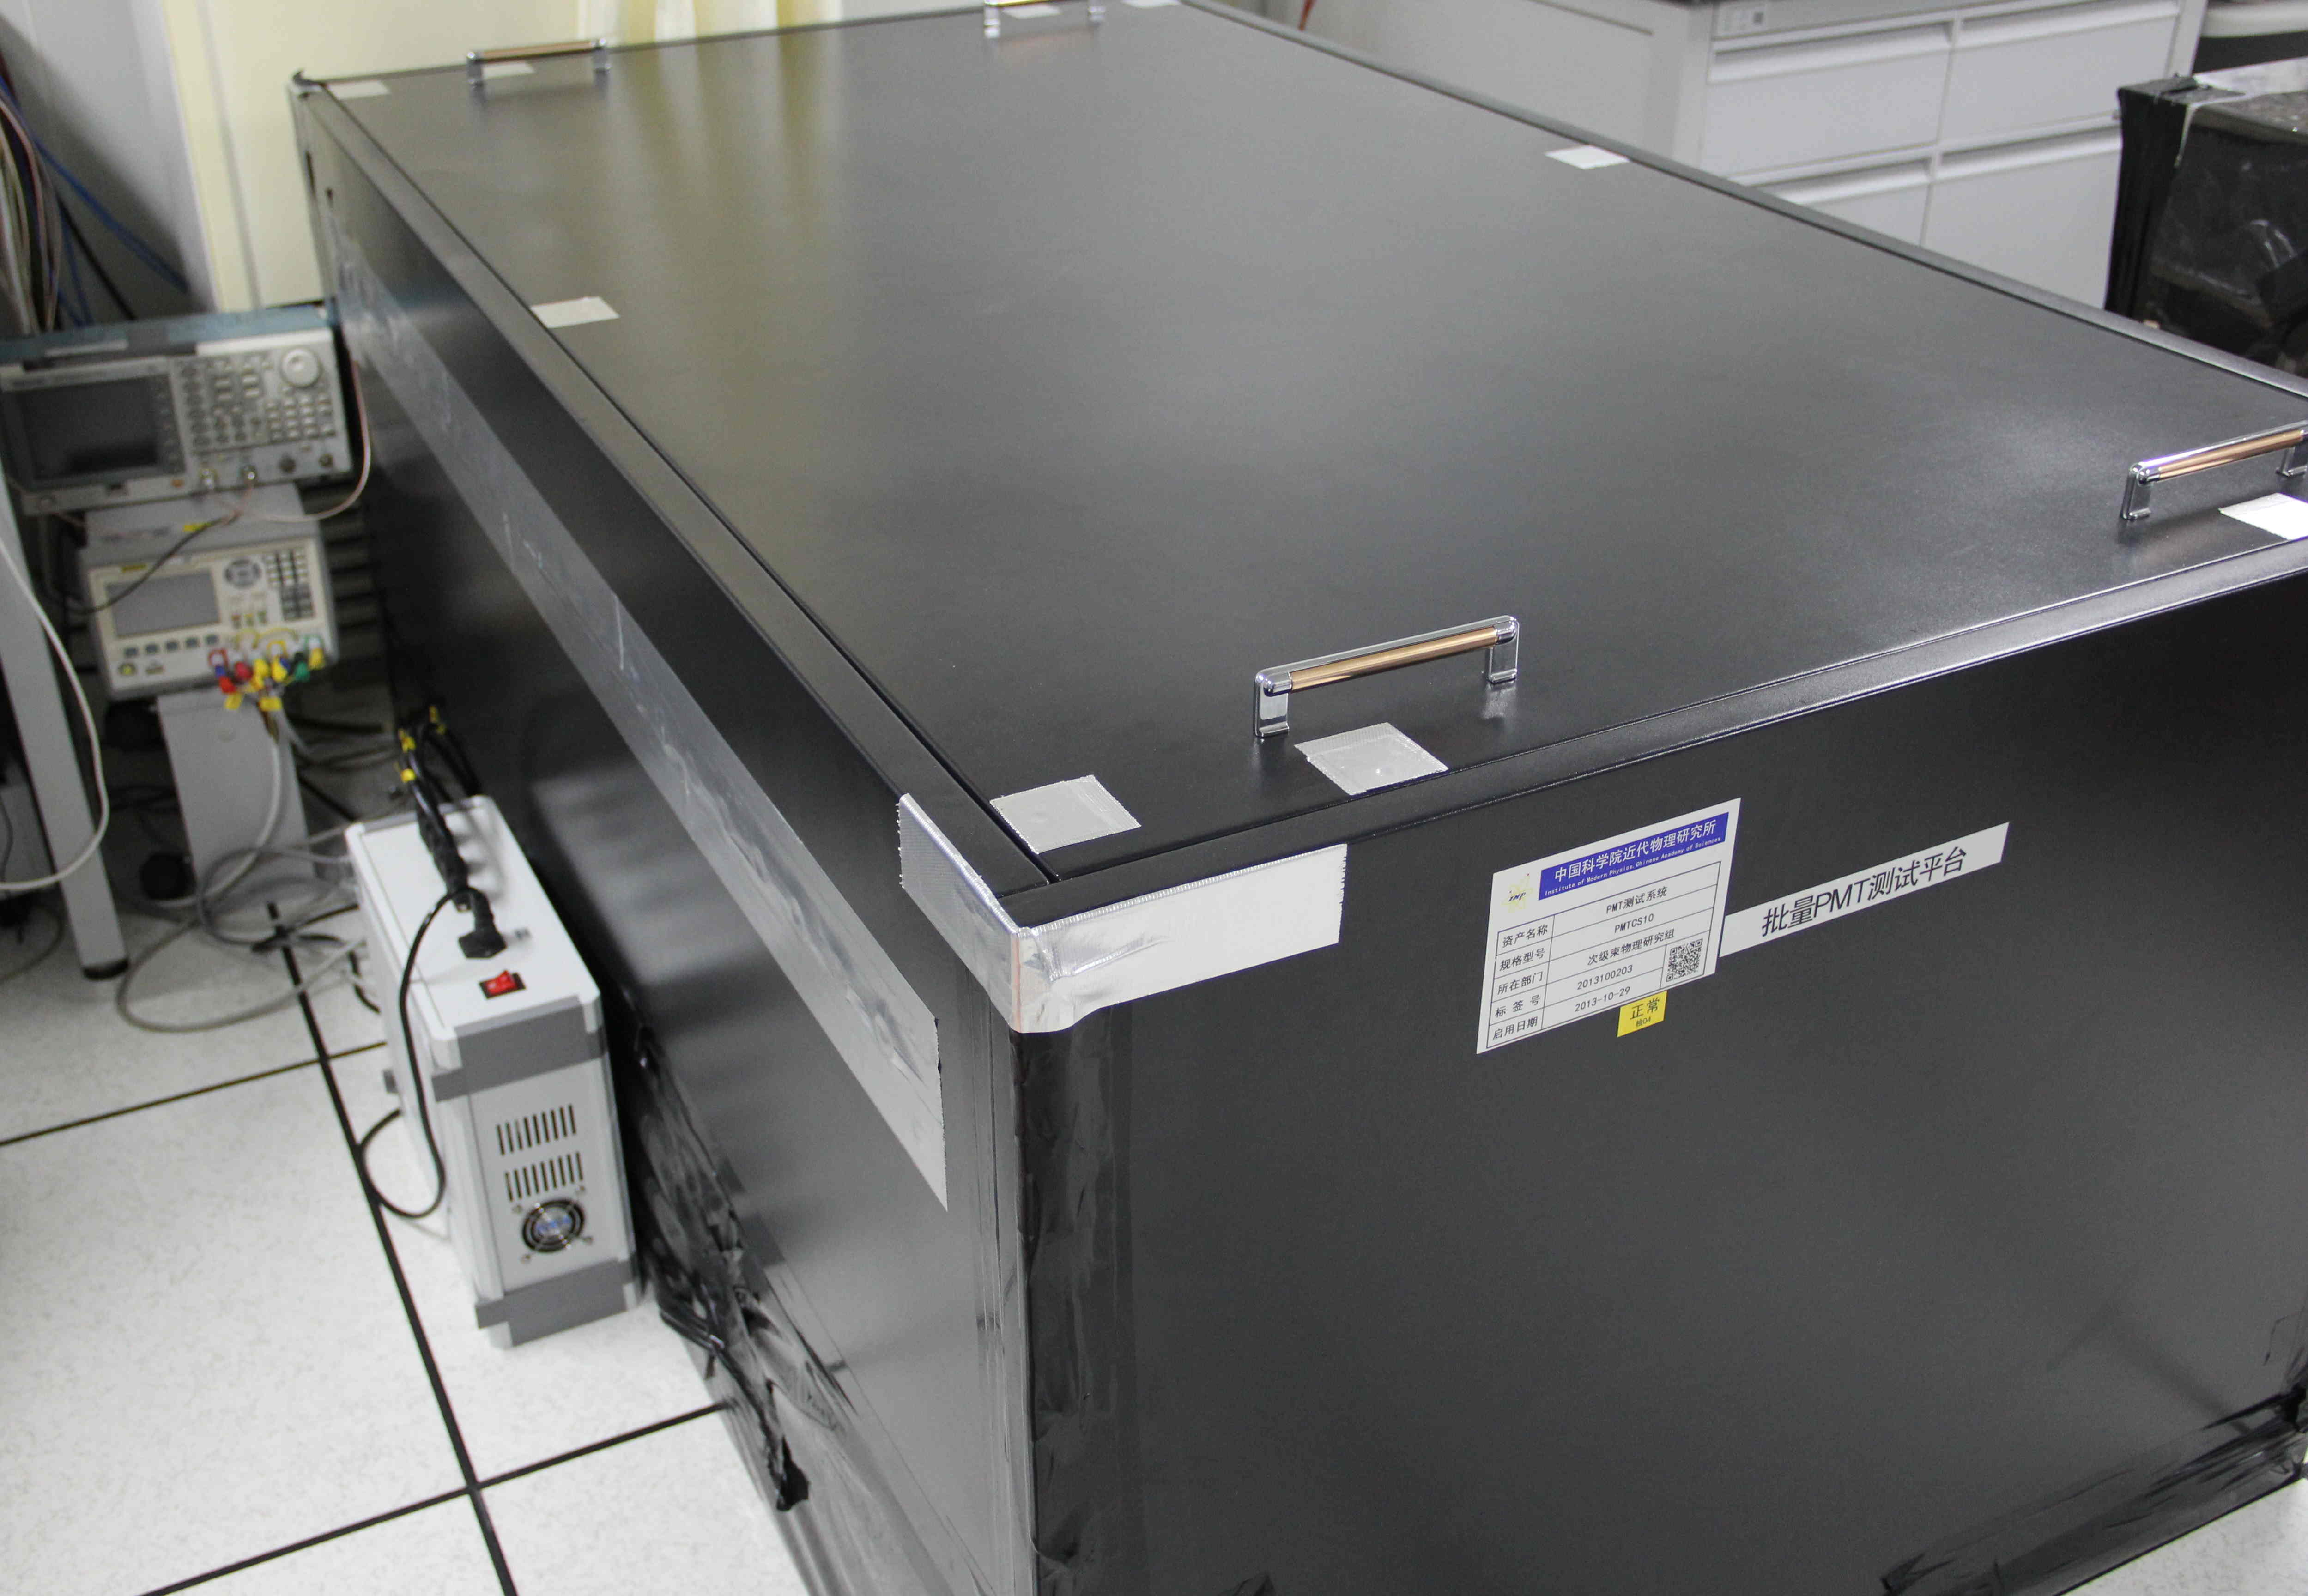
\includegraphics[width=0.49\textwidth]{chap/pmt_test/fig/black_box.jpg}
	}
	\subfloat[][三维移动平台与固定平台]{
		\label{fig:pmt_test:stages}
		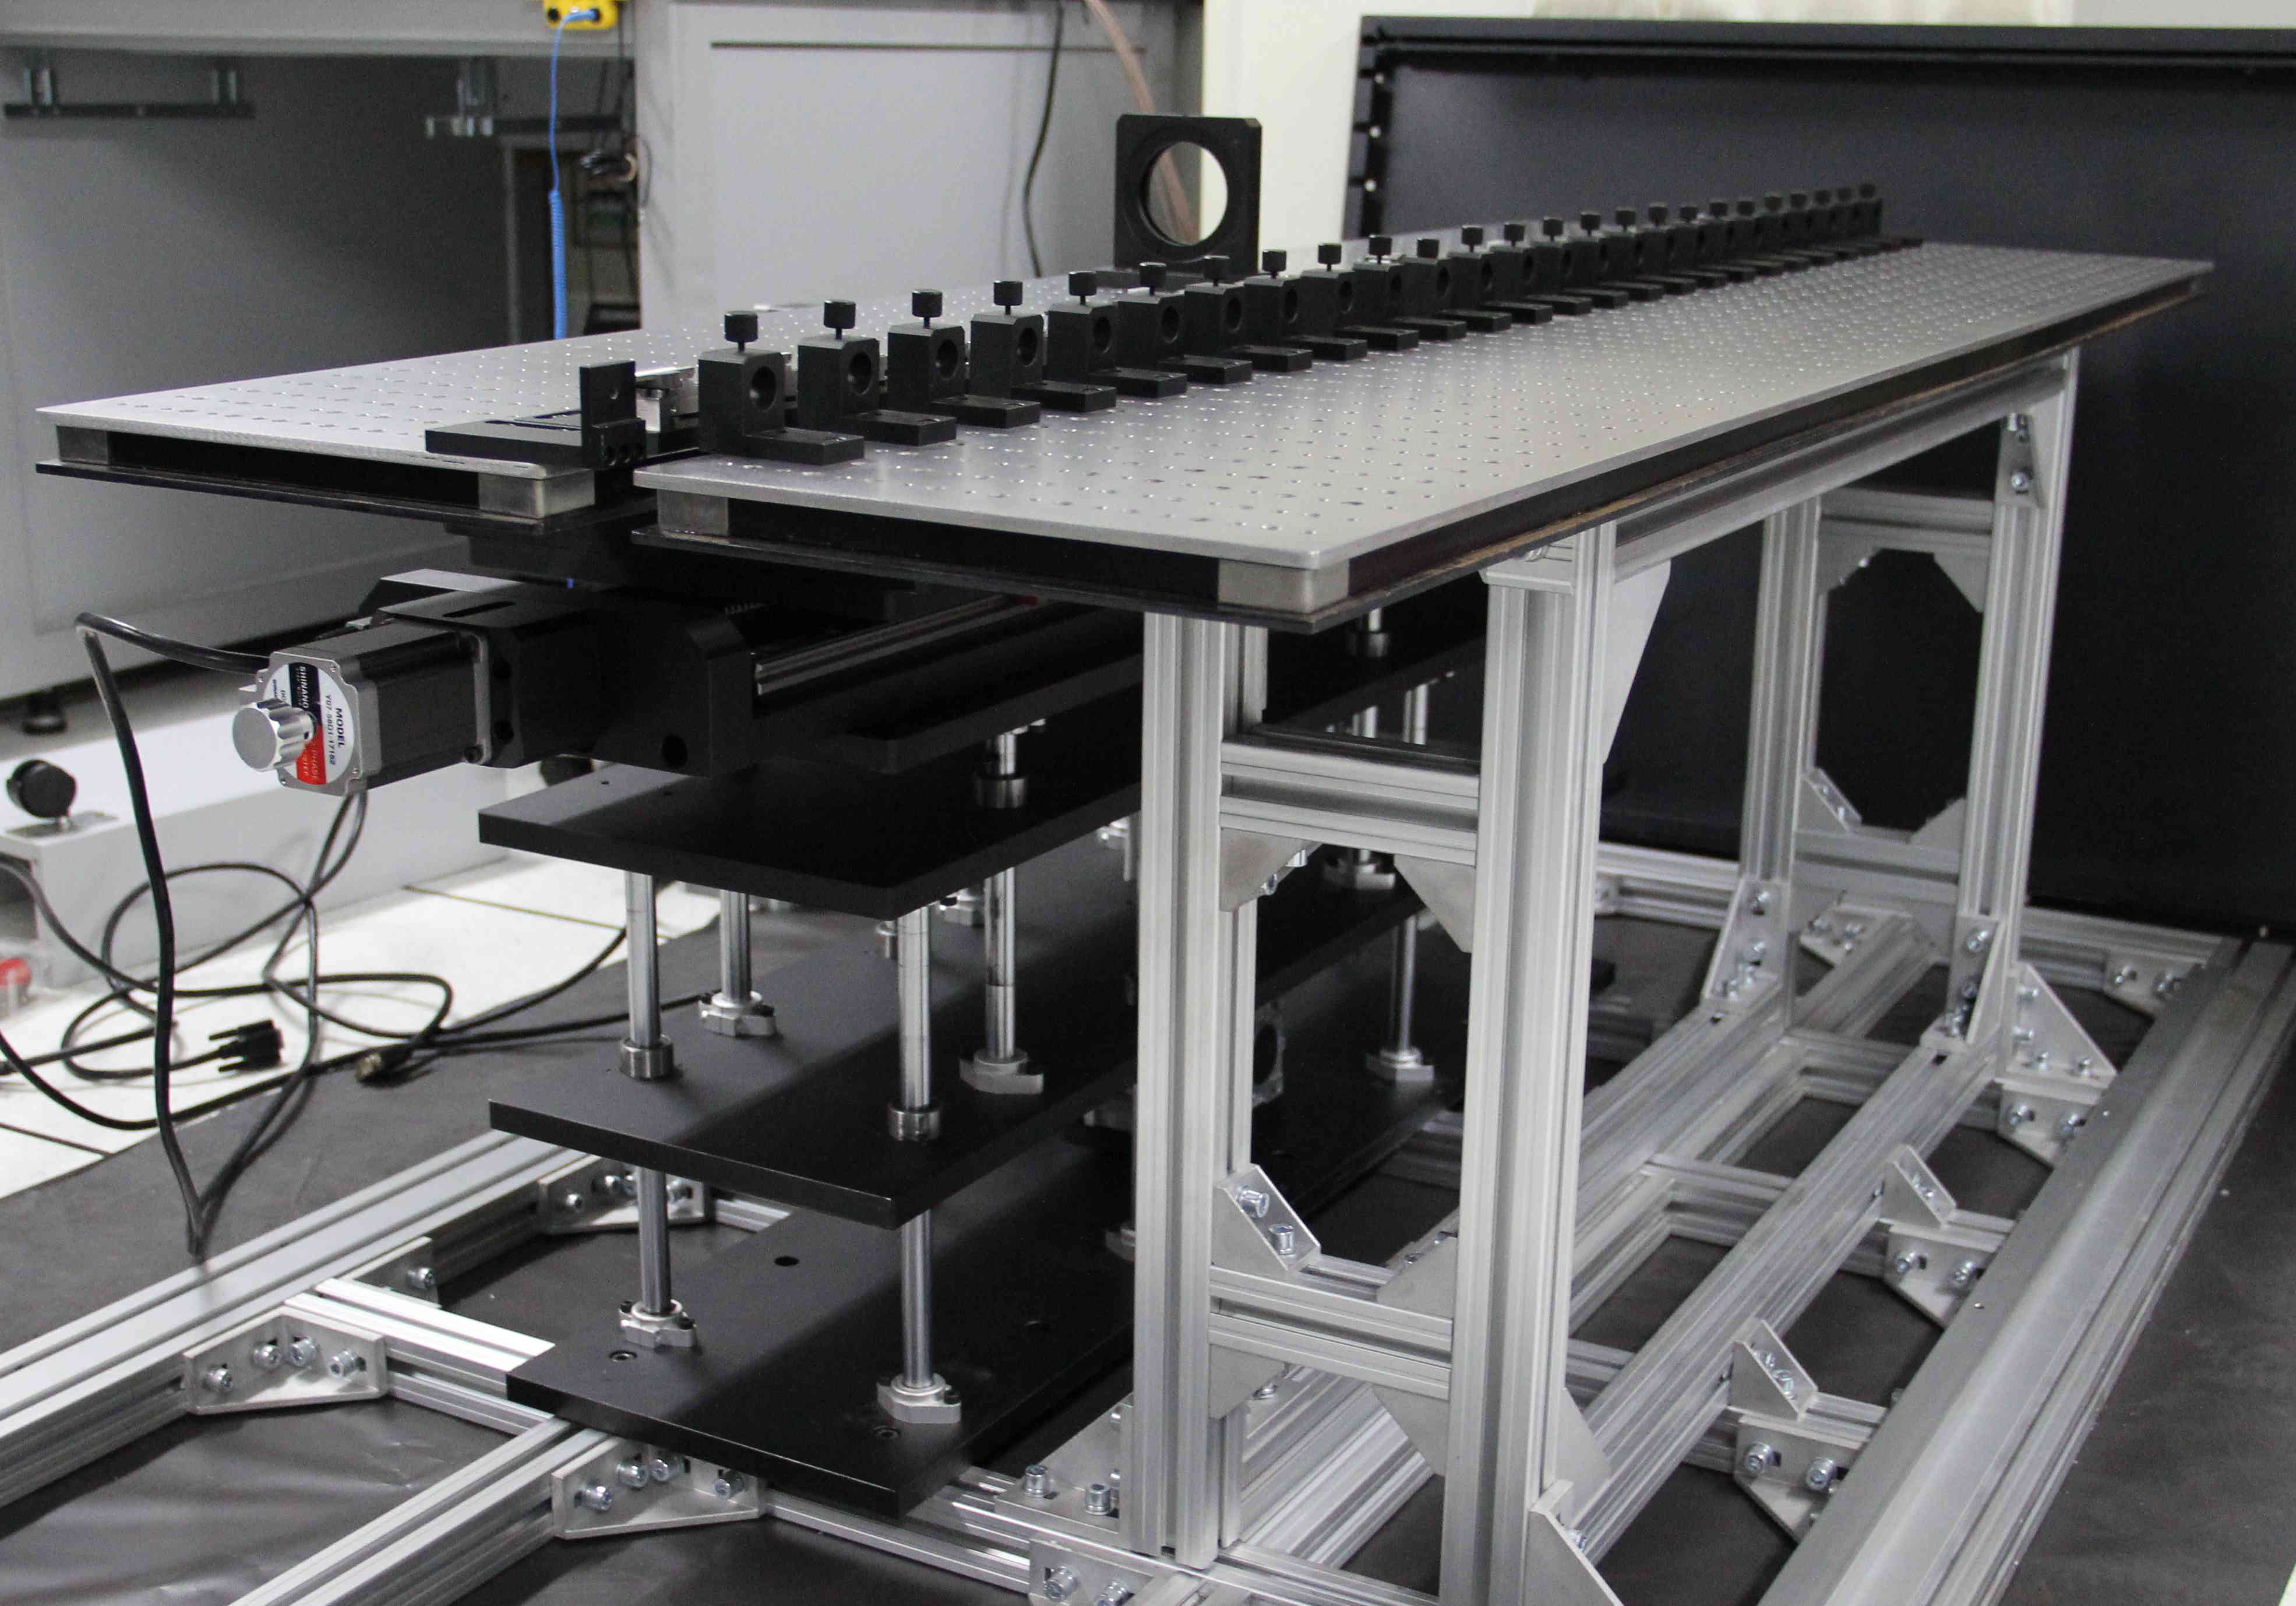
\includegraphics[width=0.49\textwidth]{chap/pmt_test/fig/stages.jpg}
	}
	\caption{PMT批量测试平台的主体结构}
	\label{fig:blindfigure}
\end{figure}
两个平台的台面各覆盖有一块面积为$1560mm\times250mm$的光学平板。
平板材质为\SI{2.5}{cm}厚度的不锈钢,因此可以有效抵抗重物放置带来的形变,保持台面上各器件位置的稳定性。
另外,光学平板上布满成网格排布的、并有M4和M6两种规格的螺纹孔,这不仅方便了台面上器件的安装与拆卸,并且提供了额外的摆放灵活性。
三维移动平台可以带动台面完成X-Y-Z三个方向的移动,每个方向都用一个步进电机驱动,其最大负载重量为\SI{30}{\kilo\gram}。
表\ref{tab:pmt_test:motorized_stage}列出了它的基本运动参数。
可以看到,平台的左右行程和上下行程使其能够对所有直径小于\SI{60}{\milli\meter}的PMT进行全面地光阴极扫描。
额外的第三维运动主要用于控制光纤与待测PMT之间的距离,在测试时尽量拉近光纤与PMT端面的距离,而在拆卸时拉远它们之间的距离,从而保护光纤不受意外损伤。
三个方向的步进电机都由一个运动控制器控制\cite{leetro},并可以利用PCI总线实现远程控制。
\begin{table}[htb]
	\centering	
	\begin{tabulary}{0.6\linewidth}{LC}
		\toprule[1.5pt]
		\textbf{项目} & \textbf{数值}	\\ 
		\midrule[1pt]
		最小步长		& \SI{1.56}{\micro\meter}	\\
		左右行程		& \SI{60}{\milli\meter}	\\
		上下行程		& \SI{70}{\milli\meter}	\\
		前后行程		& \SI{15}{\milli\meter}	\\
		\bottomrule[1.5pt]
	\end{tabulary}
	\caption{三维移动平台的基本运动参数}
	\label{tab:pmt_test:motorized_stage}	
\end{table}
为了方便操作和固定位置,我们还定制了专用的PMT夹具和光纤夹头,图\ref{fig:pmt_test:fixtures}展示了R4443和光纤固定在测试平台上的状态。
其中,光纤夹头可以实现水平方向上的微调,便于将光纤对准PMT光阴极中心。
% 紧固件
\begin{figure}[htbp]
	\centering
	\includegraphics[width=0.6\textwidth]{chap/pmt_test/fig/fixtures.jpg}
	\caption{PMT夹具和光纤夹头}
	\label{fig:pmt_test:fixtures}
\end{figure}

% 光源以及驱动
PMT测试系统使用大功率的蓝光LED(\SI{3}{\watt}, \SIrange{465}{485}{\nano\meter})作为光源。
该LED的发光光谱能够与大部分光阴极材料的光谱响应相吻合,而且曾被成功应用到HIRFL-RIBLL2外靶终端的中子墙光刻度系统中\cite{yuyuhong_led},其功率大小能够满足大量光通路的驱动要求。
为了使LED产生脉冲光,我们采用通用的脉冲发生器AFG3252\cite{afg3252}产生的方波信号来直接驱动LED发光。
虽然AFG3252不是专用的LED驱动器,但它的驱动效果能够满足我们的基本需求,如图\ref{fig:pmt_test:led_pulse}所示。
\begin{figure}[htbp]
	\centering
	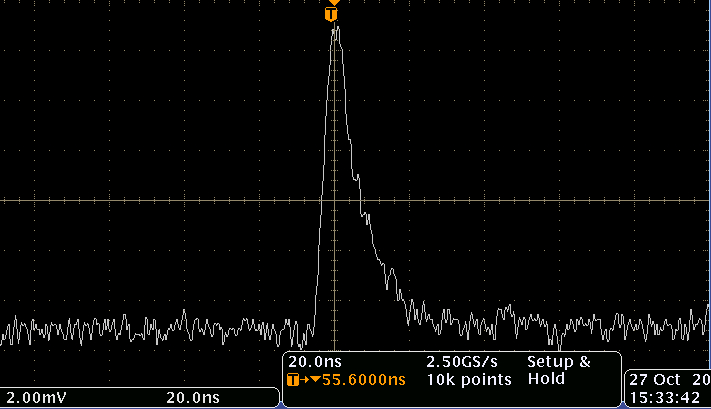
\includegraphics[width=0.65\textwidth]{chap/pmt_test/fig/led_pulse.jpg}
	\caption{\SI{30}{\nano\second}脉宽,\SI{5}{\nano\second}上升沿/下降沿的方波脉冲驱动LED发光得到的R4443输出波形}
	\label{fig:pmt_test:led_pulse}
\end{figure}
AFG3252的驱动脉冲参数可以在很大的范围内进行调整,而且精度很高,这是专用的LED驱动器达不到,因此可以满足各种各样的光输出要求,增强了PMT测试平台的通用性。
图\ref{fig:pmt_test:led_response}给出了不同脉宽、不同幅度的方波产生的LED光强变化,可以看到脉冲幅度与LED的输出光强并不成正比,这需要在使用中特别加以注意。
\begin{figure}[htbp]
	\centering
	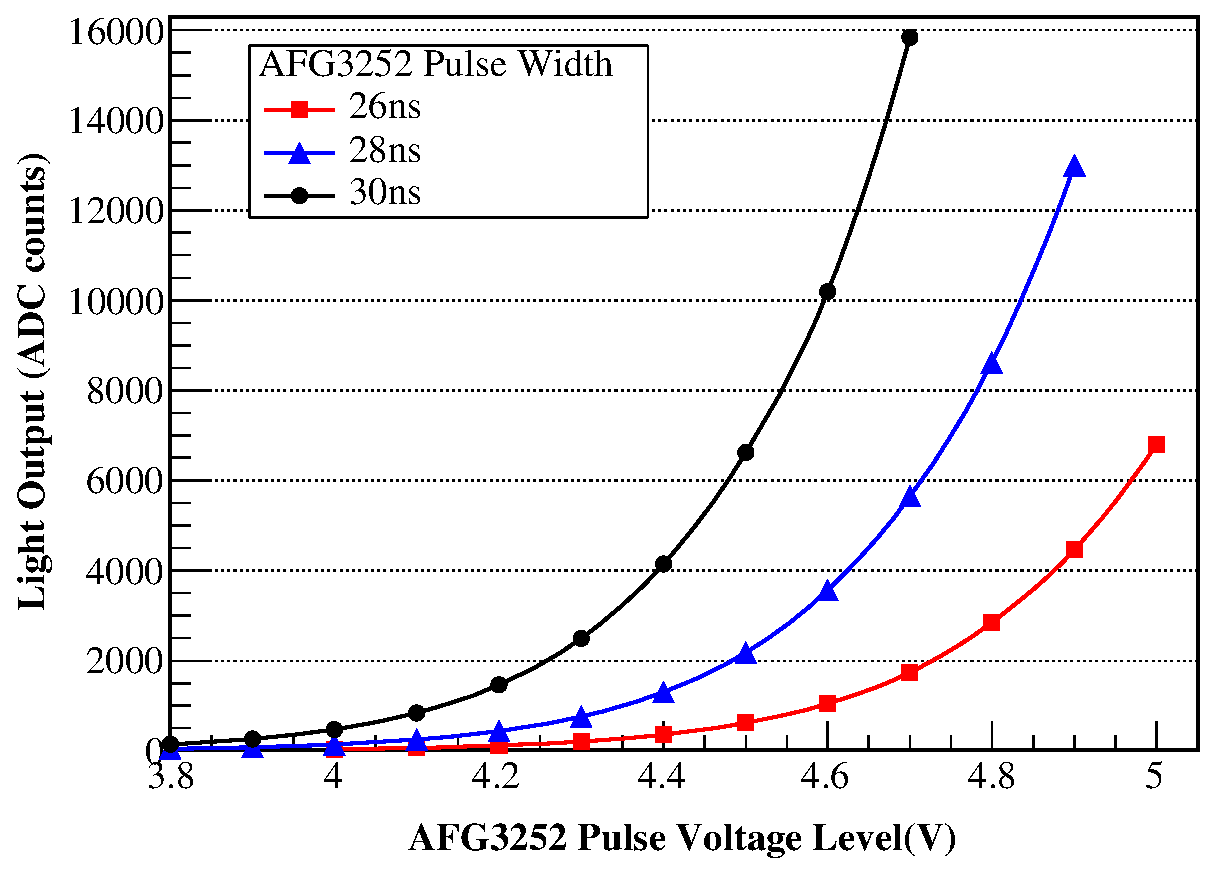
\includegraphics[width=0.7\textwidth]{chap/pmt_test/fig/led_response.eps}
	\caption{LED输出脉冲的光强度与AFG3253脉冲幅度的非线性关系}
	\label{fig:pmt_test:led_response}
\end{figure}
AFG3252的另外一个优点是:它的所有功能都可以在远程进行控制,而且接口丰富,我们可以选择熟悉的方式对其进行控制。
在PMT批量测试系统中,我们通过网口,并使用SCPI(Standard Commands for Programmable Instruments)命令\cite{afg3000_programmer_manual}对AFG3252进行远程操作。

% 积分球
LED发出的光脉冲通过集束光纤被分配到各支PMT,它与集束光纤之间通过一个\SI{5}{\centi\meter}的积分球耦合。LED、积分球和集束光纤一起构成了PMT测试系统的光分配系统,如图\ref{fig:pmt_test:light_distribution}。
其中LED通过导热硅胶固定在一个与积分球入射端口适配的底座上,而集束光纤通过三维位移台直接对准积分球出射端口的中心(参加见图\ref{fig:pmt_test:lightsource_integration})。
\begin{figure}[htbp]
	\centering
	\subfloat[][1)LED 2)积分球 3)集束光纤]{
		\label{fig:pmt_test:lightsource_components}
		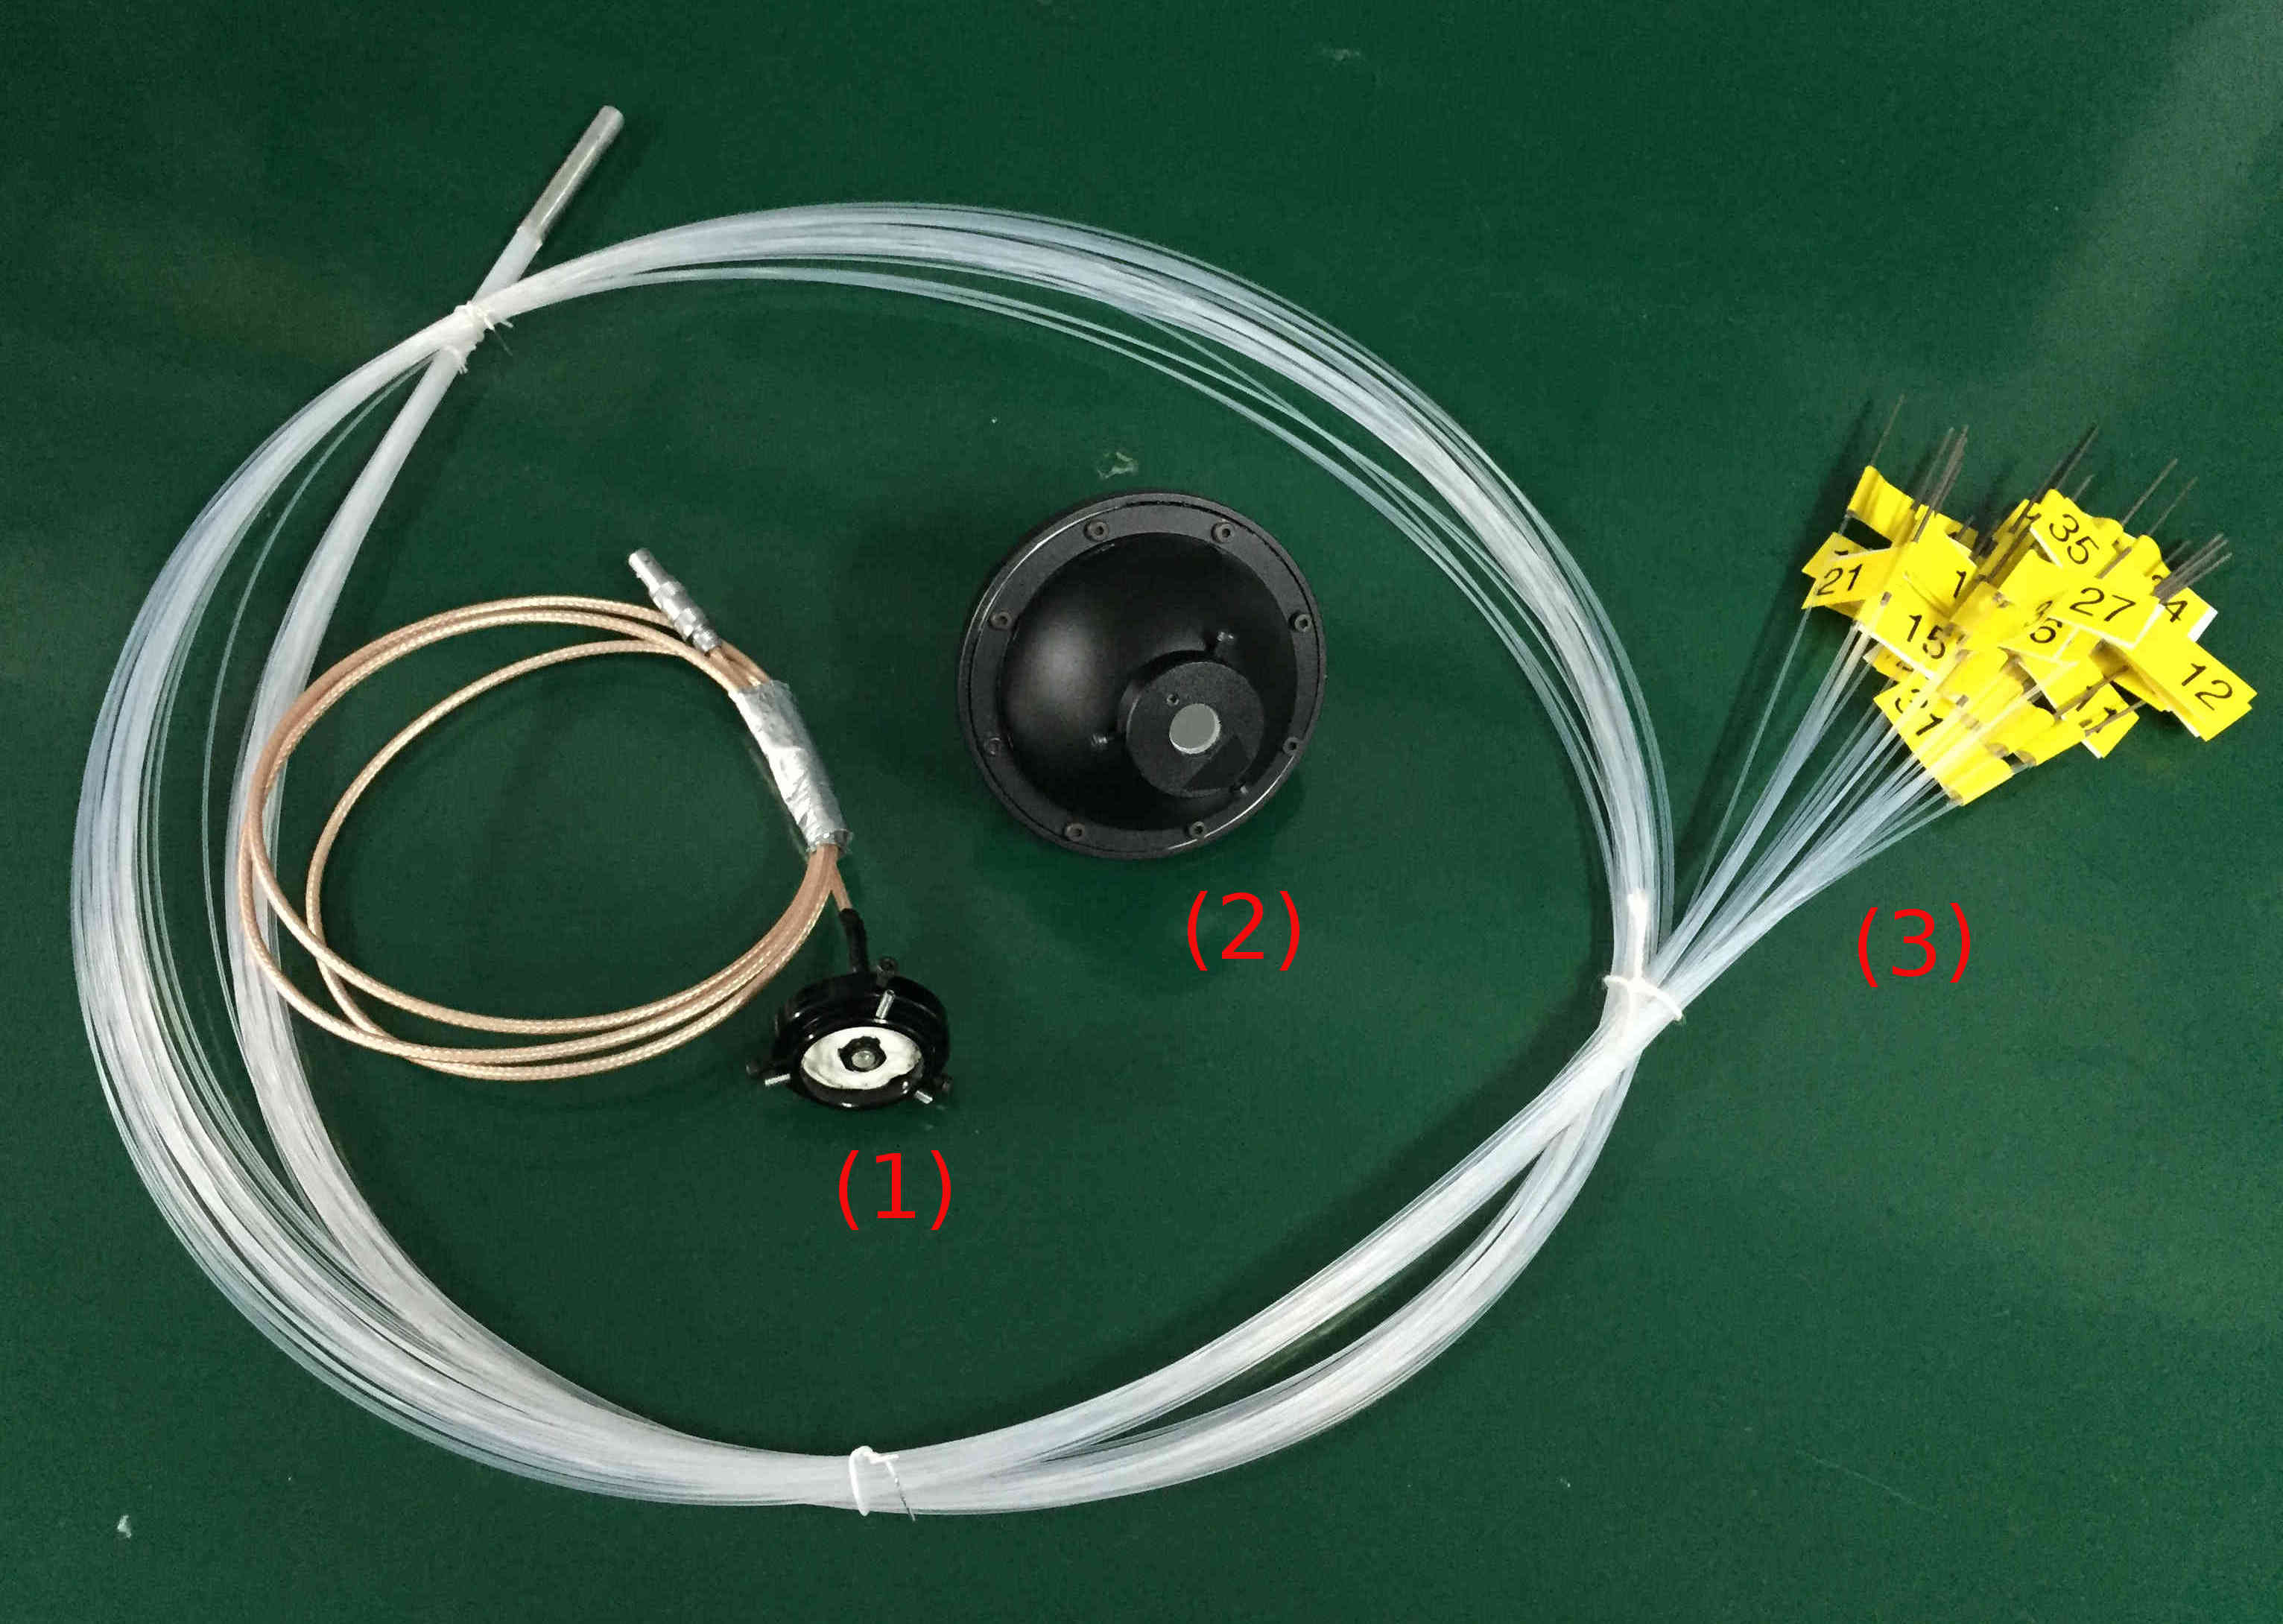
\includegraphics[width=0.49\textwidth]{chap/pmt_test/fig/lightsource_components.jpg}
	}
	\subfloat[][各组件耦合在一起]{
		\label{fig:pmt_test:lightsource_integration}
		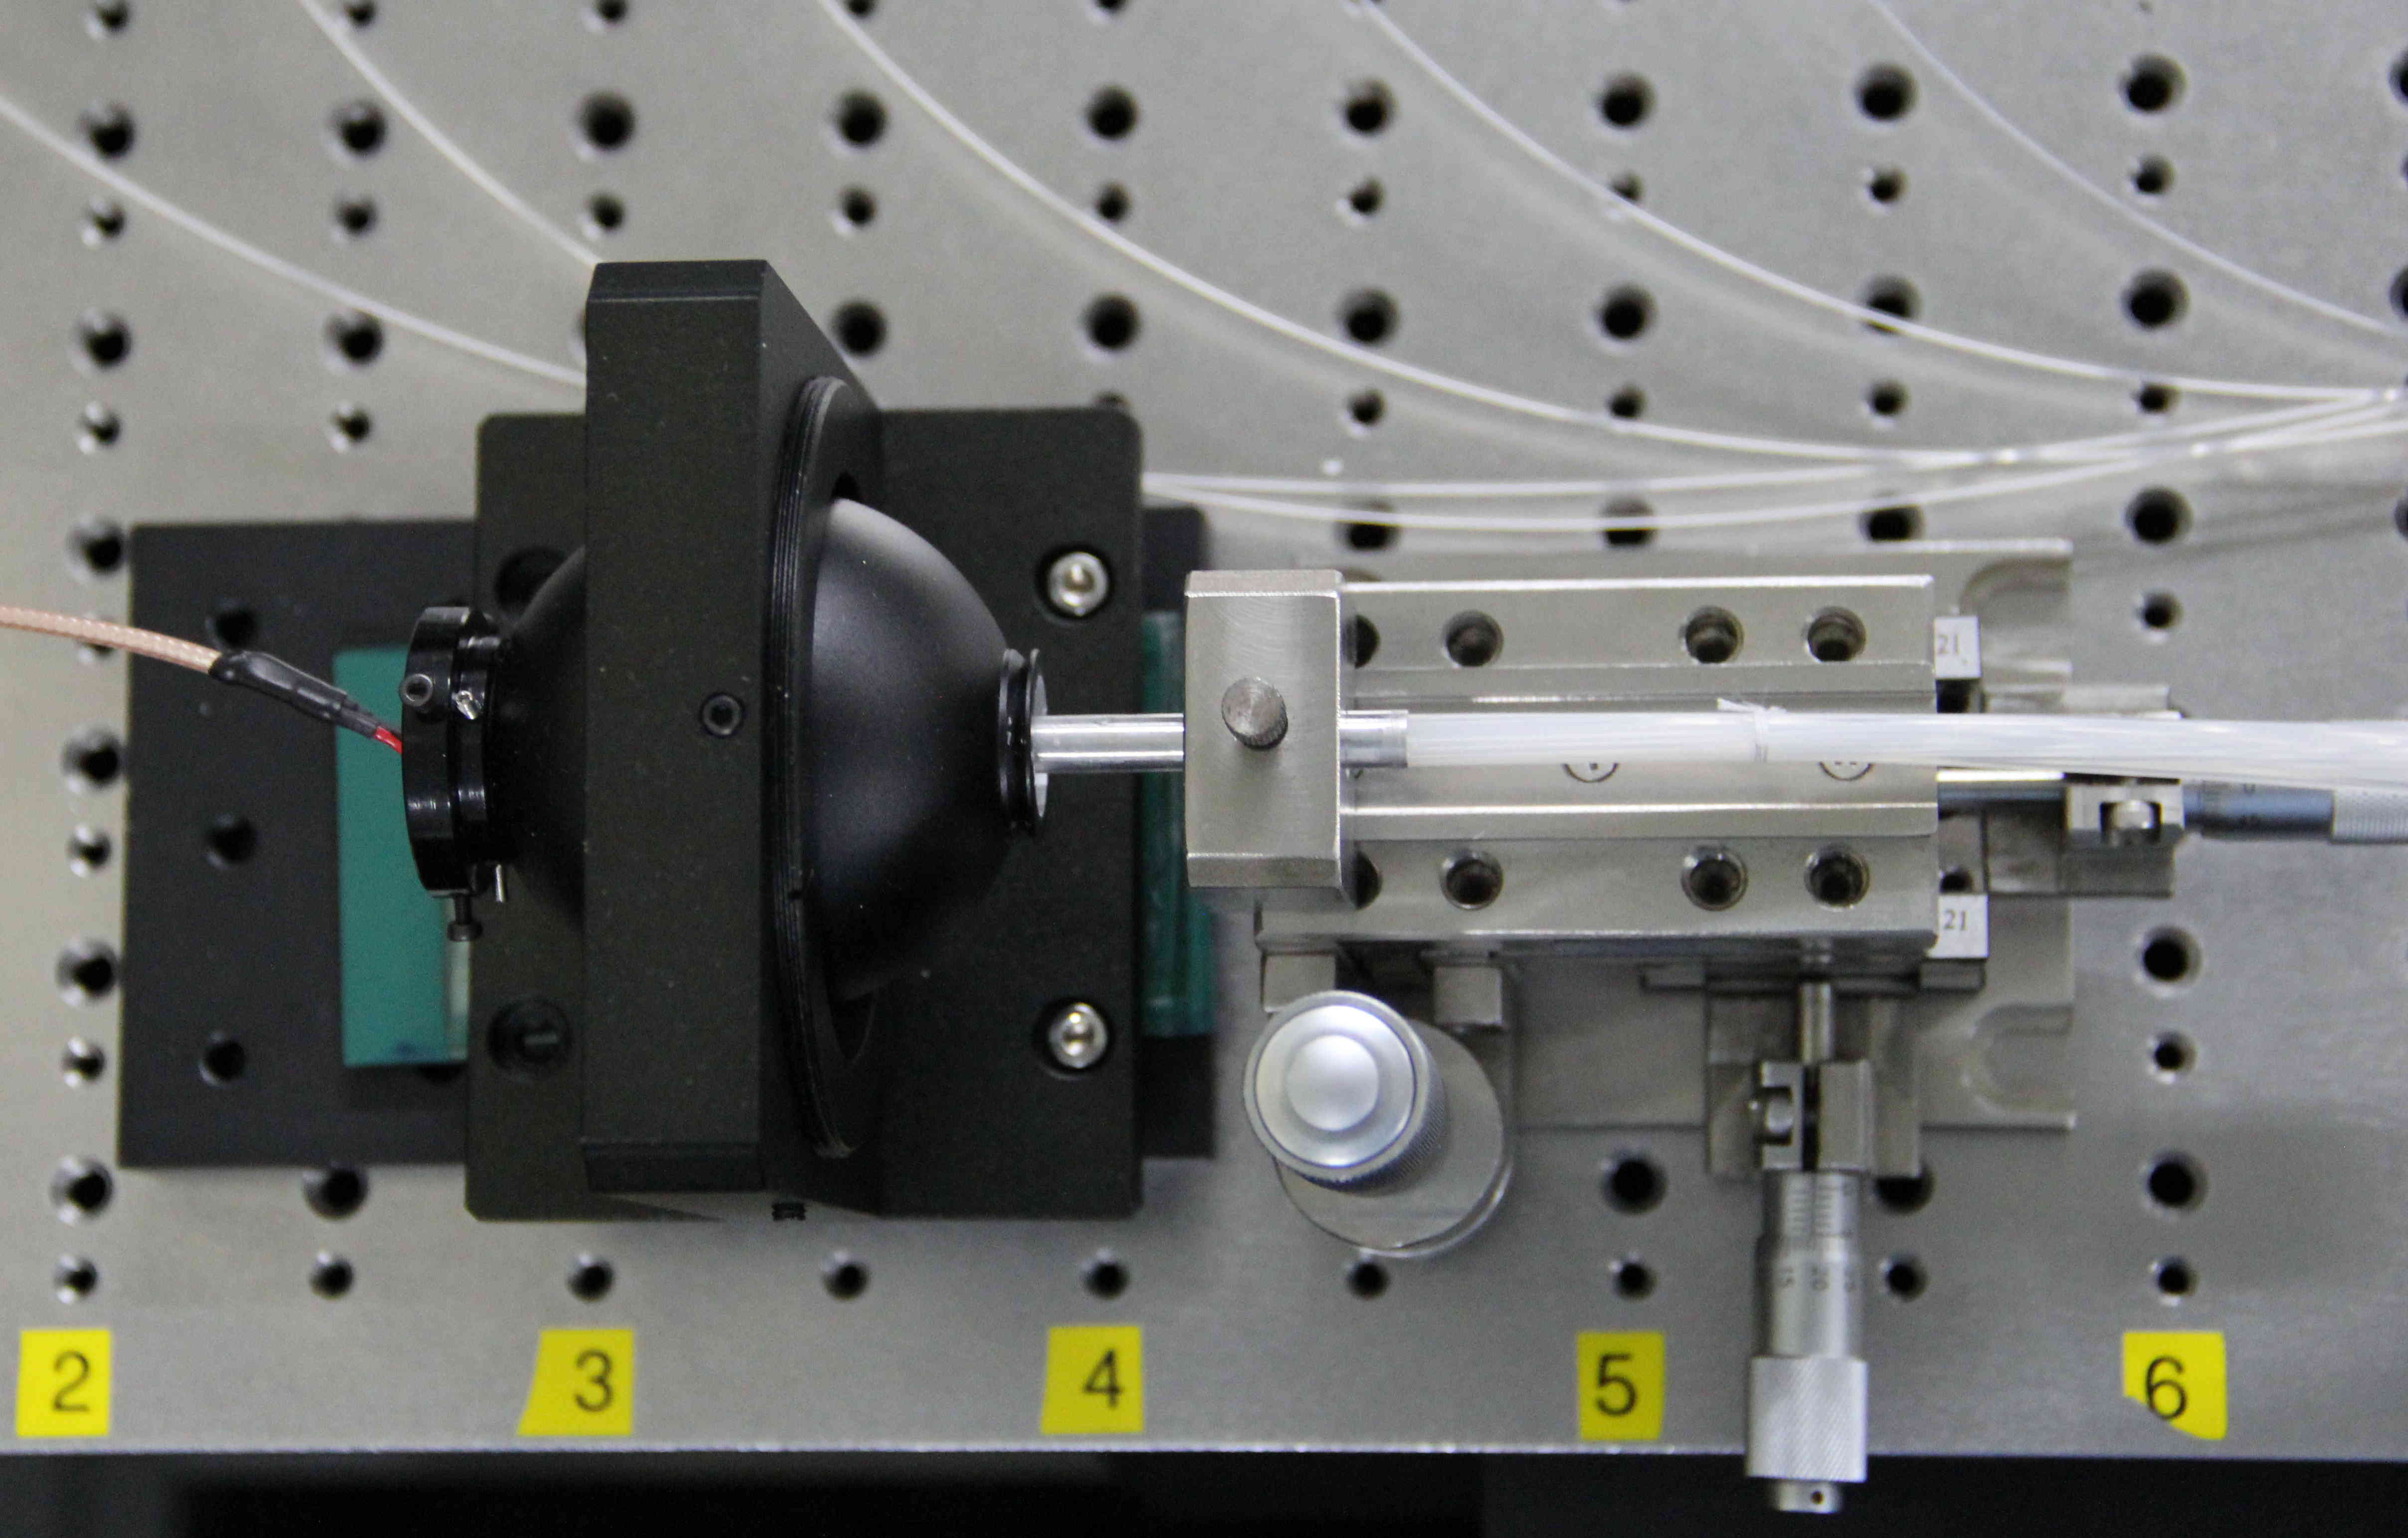
\includegraphics[width=0.49\textwidth]{chap/pmt_test/fig/lightsource_integration.jpg}
	}		
	\caption{PMT批量测试平台的光源与光分配系统}
	\label{fig:pmt_test:light_distribution}
\end{figure}
积分球是一个具有高反射性内表面涂层的空心球体,它是一个理想的光积分器件,入射光在其内部经过多次反射后,能够在其出射端口均匀出射。
积分器在此处的应用主要出于两点考虑:1)我们希望各条光通路具有相近的光输出强度;2)将
我们使用的积分球\cite{integrating_sphere}使用的内壁涂层材料为$BaSO_4$,蓝光反射率达到\SI{98.5}{\percent},因此即便它的半径较小,却仍然能够得到较好的均匀性。
在LED固定到积分球入射端口后,我们对积分球出射端口的光强度进行了“十”字扫描,结果显示其光均匀性可以达到$\pm\SI{0.5}{\percent}$,如图\ref{fig:pmt_test:integrationsphere_uniformity}所示。
\begin{figure}[htbp]
	\centering
	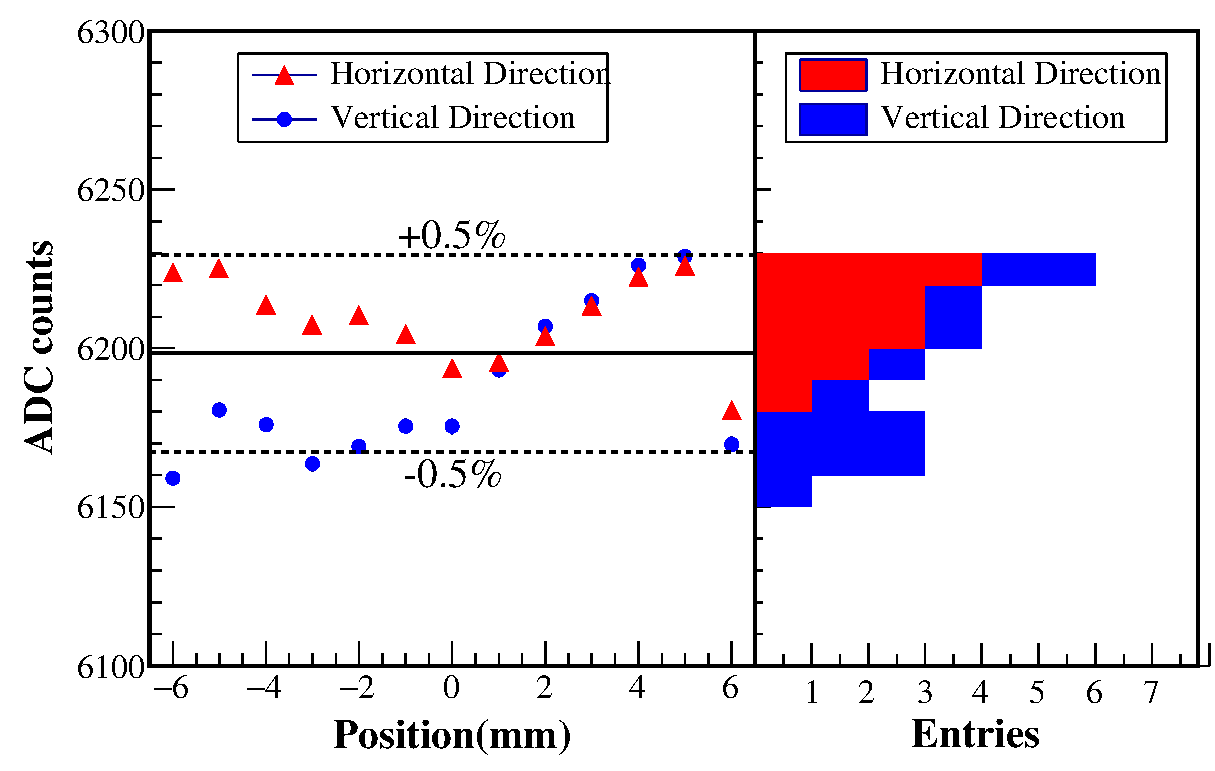
\includegraphics[width=0.65\textwidth]{chap/pmt_test/fig/integrationsphere_uniformity.eps}
	\caption{\SI{5}{cm}铝合金积分球输出端口的光均匀性}
	\label{fig:pmt_test:integrationsphere_uniformity}
\end{figure}





% 集束光纤
我们使用集束光纤将来自光源的光脉冲分配到各支PMT,集束光纤耦合在积分球的输出端口,它们一起构成了PMT测试系统的光分配系统。
\begin{figure}[htbp]
	\centering
	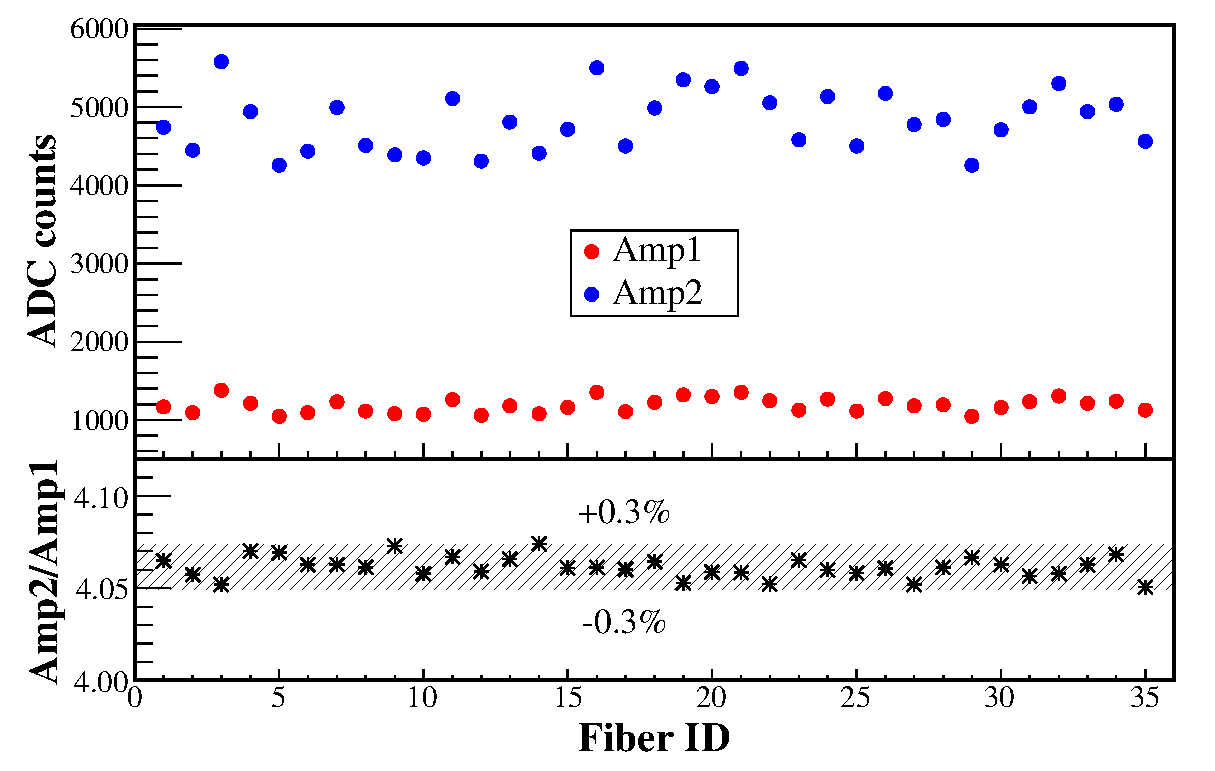
\includegraphics[width=0.7\textwidth]{chap/pmt_test/fig/fiber_difference.eps}
	\caption{集束光纤各通道的光传输差异性}
	\label{fig:pmt_test:fiber_difference}
\end{figure}

\subsection{测控软件}
% 最好这里做一个归纳性的介绍,具体细节设计放到附录中


\section{R4443裸管的性能测试}
\label{sec:pmt_test:characterization}

\subsection{相对增益的测量}
\subsection{Dynode8/Dynode5增益比值的测量}
\subsection{光阴极均匀性}
\subsection{PMT批量测试平台的长期稳定性}

\section{PMT的筛选}

\subsection{筛选方案}
工厂参数。
% 暗电流
PMT的暗电流是指在完全黑暗且没有入射光的条件下,在光电倍增管内部流动的微小电流。
由于暗电流会使得探测器的基线展宽、噪声变大,严重的情况下甚至降低探测器的能量分辨率,因此暗电流越小越好。
光电倍增管的光阴极材料是引起暗电流的主要因素。
PSD采用的R4443型号(即MOD2)使用低噪声的碱金属材料作为光阴极,从而极大地抑制了暗电流的大小。
根据Hamamatsu提供的出厂测试信息,我们发现所有管子的暗电流都小于PSD的要求。
% 增益
R4443的Dy8通道用于覆盖PSD动态范围的低端部分,主要用于$e/\gamma$;R4443的Dy5通道用于覆盖PSD动态范围的高端部分,主要用于相对论重离子的电荷测量。
我们希望Dy8的增益尽量高,使其测得的MIP信号尽量与基线噪声相分离,从而降低$e/\gamma$误判率。
另一方面,PSD对整体的动态范围有严格的区间要求($\SI{0.1}{MIPs}\sim\SI{1400}{MIPs}$),过高的Dy8增益会压低Dy5的增益(即提高了Dy58比值),从而降低Dy5对重离子电荷的分辨能力。
因此
\subsection{参考单元模块的MIPs响应}
\subsection{与塑闪单元条的匹配}
	% 各章节。
	\chapter{塑闪阵列探测器的建造}
\label{ch:construction}
相比于地面使用,空间项目对探测器提出了具有更加苛刻的使用条件和更加严格的质量要求。
这不仅意味着要对探测器各部件进行特殊设计以适应火箭发射和空间使用环境,而且探测器的组件生产和整体装配必须遵循一定的建造规范并辅以严格的质量控制程序以保证其达到设计要求和质量。
塑闪阵列探测器的具体设计已经在第\ref{ch:description}章进行了梳理,本章将对它的实际建造过程进行简单介绍。

指导塑闪阵列探测器建造的有两条基本原则:一是要实现其功能要求,二是满足其质量要求。
PSD由探测器主体功能模块,高压扇出模块,前端电子学模块以及机械支撑模块这四部分组成。
其中,高压扇出模块、前端电子学模块和机械支撑模块都由专业的外包单位负责其建造和质量控制,实验室中我们只负责探测器主体功能模块中各探测单元的建造,主要包括是PMT组件以及塑闪单元条组件。
我们还在实验室中将上述四个模块组装成探测器整体,最终完成了塑闪阵列探测器的建造工作。

\section{PMT的筛选}
\label{sec:construction:pmt_selection}
PMT筛选的原则

PMT筛选的原理:宇宙线测试参考管子

工厂参数(暗电流与Drift)
去除尺寸和外观检查不合格(光阴极和玻管表面有瑕疵)
去除参与了厂家力学检测

去除极端增益:计算对应于Dy8=700道时的工作电压,去除小于790大于930V的PMT
确定额定工作电压:设定工作电压为810,840,870,900四个档位,分别计算对应的增益,至少有一个电压在600-800之间
选择动态范围:由$1000\cdot Dy58 / Gain$计算额定工作电压下的动态范围,选择$600\sim900$之间的
去除增益随电压变化异常的:计算额定工作电压加90V后的增益相对于原来的比值,选择$1.6\sim 2$之间的

570测试-190挑选焊接-164安装

% 暗电流
PMT的暗电流是指在完全黑暗且没有入射光的条件下,在光电倍增管内部流动的微小电流。
由于暗电流会使得探测器的基线展宽、噪声变大,严重的情况下甚至降低探测器的能量分辨率,因此暗电流越小越好。
光电倍增管的光阴极材料是引起暗电流的主要因素。
PSD采用的R4443型号(即MOD2)使用低噪声的碱金属材料作为光阴极,从而极大地抑制了暗电流的大小。
根据Hamamatsu提供的出厂测试信息,我们发现所有管子的暗电流都小于PSD的要求。
% 增益
R4443的Dy8通道用于覆盖PSD动态范围的低端部分,主要用于$e/\gamma$;R4443的Dy5通道用于覆盖PSD动态范围的高端部分,主要用于相对论重离子的电荷测量。
我们希望Dy8的增益尽量高,使其测得的MIP信号尽量与基线噪声相分离,从而降低$e/\gamma$误判率。
另一方面,PSD对整体的动态范围有严格的区间要求($\SI{0.1}{MIPs}\sim\SI{1400}{MIPs}$),过高的Dy8增益会压低Dy5的增益(即提高了Dy58比值),从而降低Dy5对重离子电荷的分辨能力。
因此

\section{PMT组件的生产}
\label{sec:construction:pmt_production}

\begin{figure}[htbp]
	\centering
	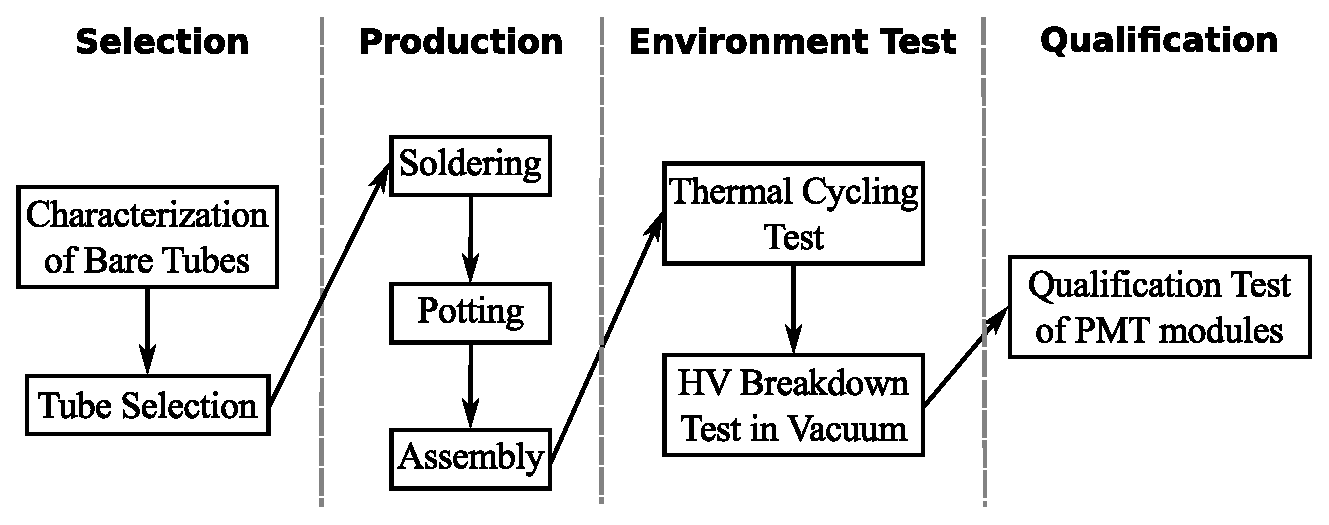
\includegraphics[width=0.95\textwidth]{chap/construction/fig/pmt_production_procedure.eps}
	\caption{PMT组件的生产流程}
	\label{fig:construction:pmt_production_procedure}
\end{figure}

\subsection{结构简介}
\label{sec:construction:pmt_assembly}

\subsection{生产流程}
\label{sec:construction:pmt_procedure}
\begin{enumerate}
	\item PMT的base焊接,信号线+信号头。
	\item 检测:电压、电容。
	\item 灌胶。
	\item 高低温循环。
	\item 真空高压测试。
	\item PMT测试平台测试
\end{enumerate}

\section{塑闪单元条的生产}
\label{sec:construction:bar_production}
测试与筛选过程与PMT正好相反,因为单元条需要包装后才能测试。

\subsection{单元条的包装与测试}
\label{sec:construction:bar_wrapping_and_test}

\subsection{单元条的筛选}
\label{sec:construction:bar_selection}
尺寸复核
热膨胀系数
技术衰减长度:平滑否-包装是否好,两端相差较大也踢出,大于一个值
响应均匀性
探测效率
MPV响应?

\section{探测器整体组装}
\label{sec:construction:psd_assembly}

\subsection{PMT与塑闪单元条的匹配}

\begin{enumerate}
	\item 布单元条。
	\item PMT组件加套筒和播磨合金
	\item 上PMT。
	\item 宇宙线测试。
	\item 上高压扇出板
	\item 上FEE盒子(焊接定位用),上FEE转接板
	\item 上高压接头
	\item 正式上FEE盒子
	\item 上FEE电路板
	\item 上顶板
\end{enumerate}

	%
	\chapter{PSD的宇宙线地面标定}
\label{ch:cosmic_ray}
PSD整体装配完成后,我们在实验室对它的各项性能指标进行了测试。
特别地,我们利用宇宙线对PSD探测单元模块进行了细致的标定测试,得到了一系列的刻度参数结果。
这些结果是PSD得到的第一批刻度参数数据集,它们是PSD进行初步能量重建的基础。

我们专门研制并搭建了一套宇宙线地面标定测试平台对PSD整体进行标定测试。
本章将简单介绍该平台的基本组成以及它在PSD宇宙线标定中的应用,同时给出了PSD地面宇宙线标定的主要结果。

\section{宇宙线地面标定测试平台}
\label{sec:cosmic_ray:cm_system}
\subsection{简介}
\label{sec:cosmic_ray:introduction}
% 结构与组成,总装图
% 基本原理
宇宙线地面标定测试平台专门为了PSD的地面标定而设计和建造的,主要提供了两个功能:1)模拟轨道真空环境;2)确定入射宇宙线径迹。
该平台的硬件组成如图\ref{fig:cosmic_ray:cm_system}所示,其主体为一个大型真空靶室,靶室大小正好可以容纳整个PSD探测器。
真空靶室的腔体上部和下部分别放置了一个多丝漂移室探测器(Multi-Wire Drift Chamber,简称MWDC)和一个塑料闪烁体触发板探测器。
上下两块大面积触发板用于标定入射宇宙线事例,而上下两个MWDC则用于测量入射宇宙线径迹。
根据得到宇宙线入射径迹,可以推出其在PSD上的击中位置;由于MWDC和触发板的面积都能够覆盖PSD的有效面积,我们能够得到PSD所有位置处的MIP响应,从而实现PSD的精细标定。
\begin{figure}[htbp]
	\centering
	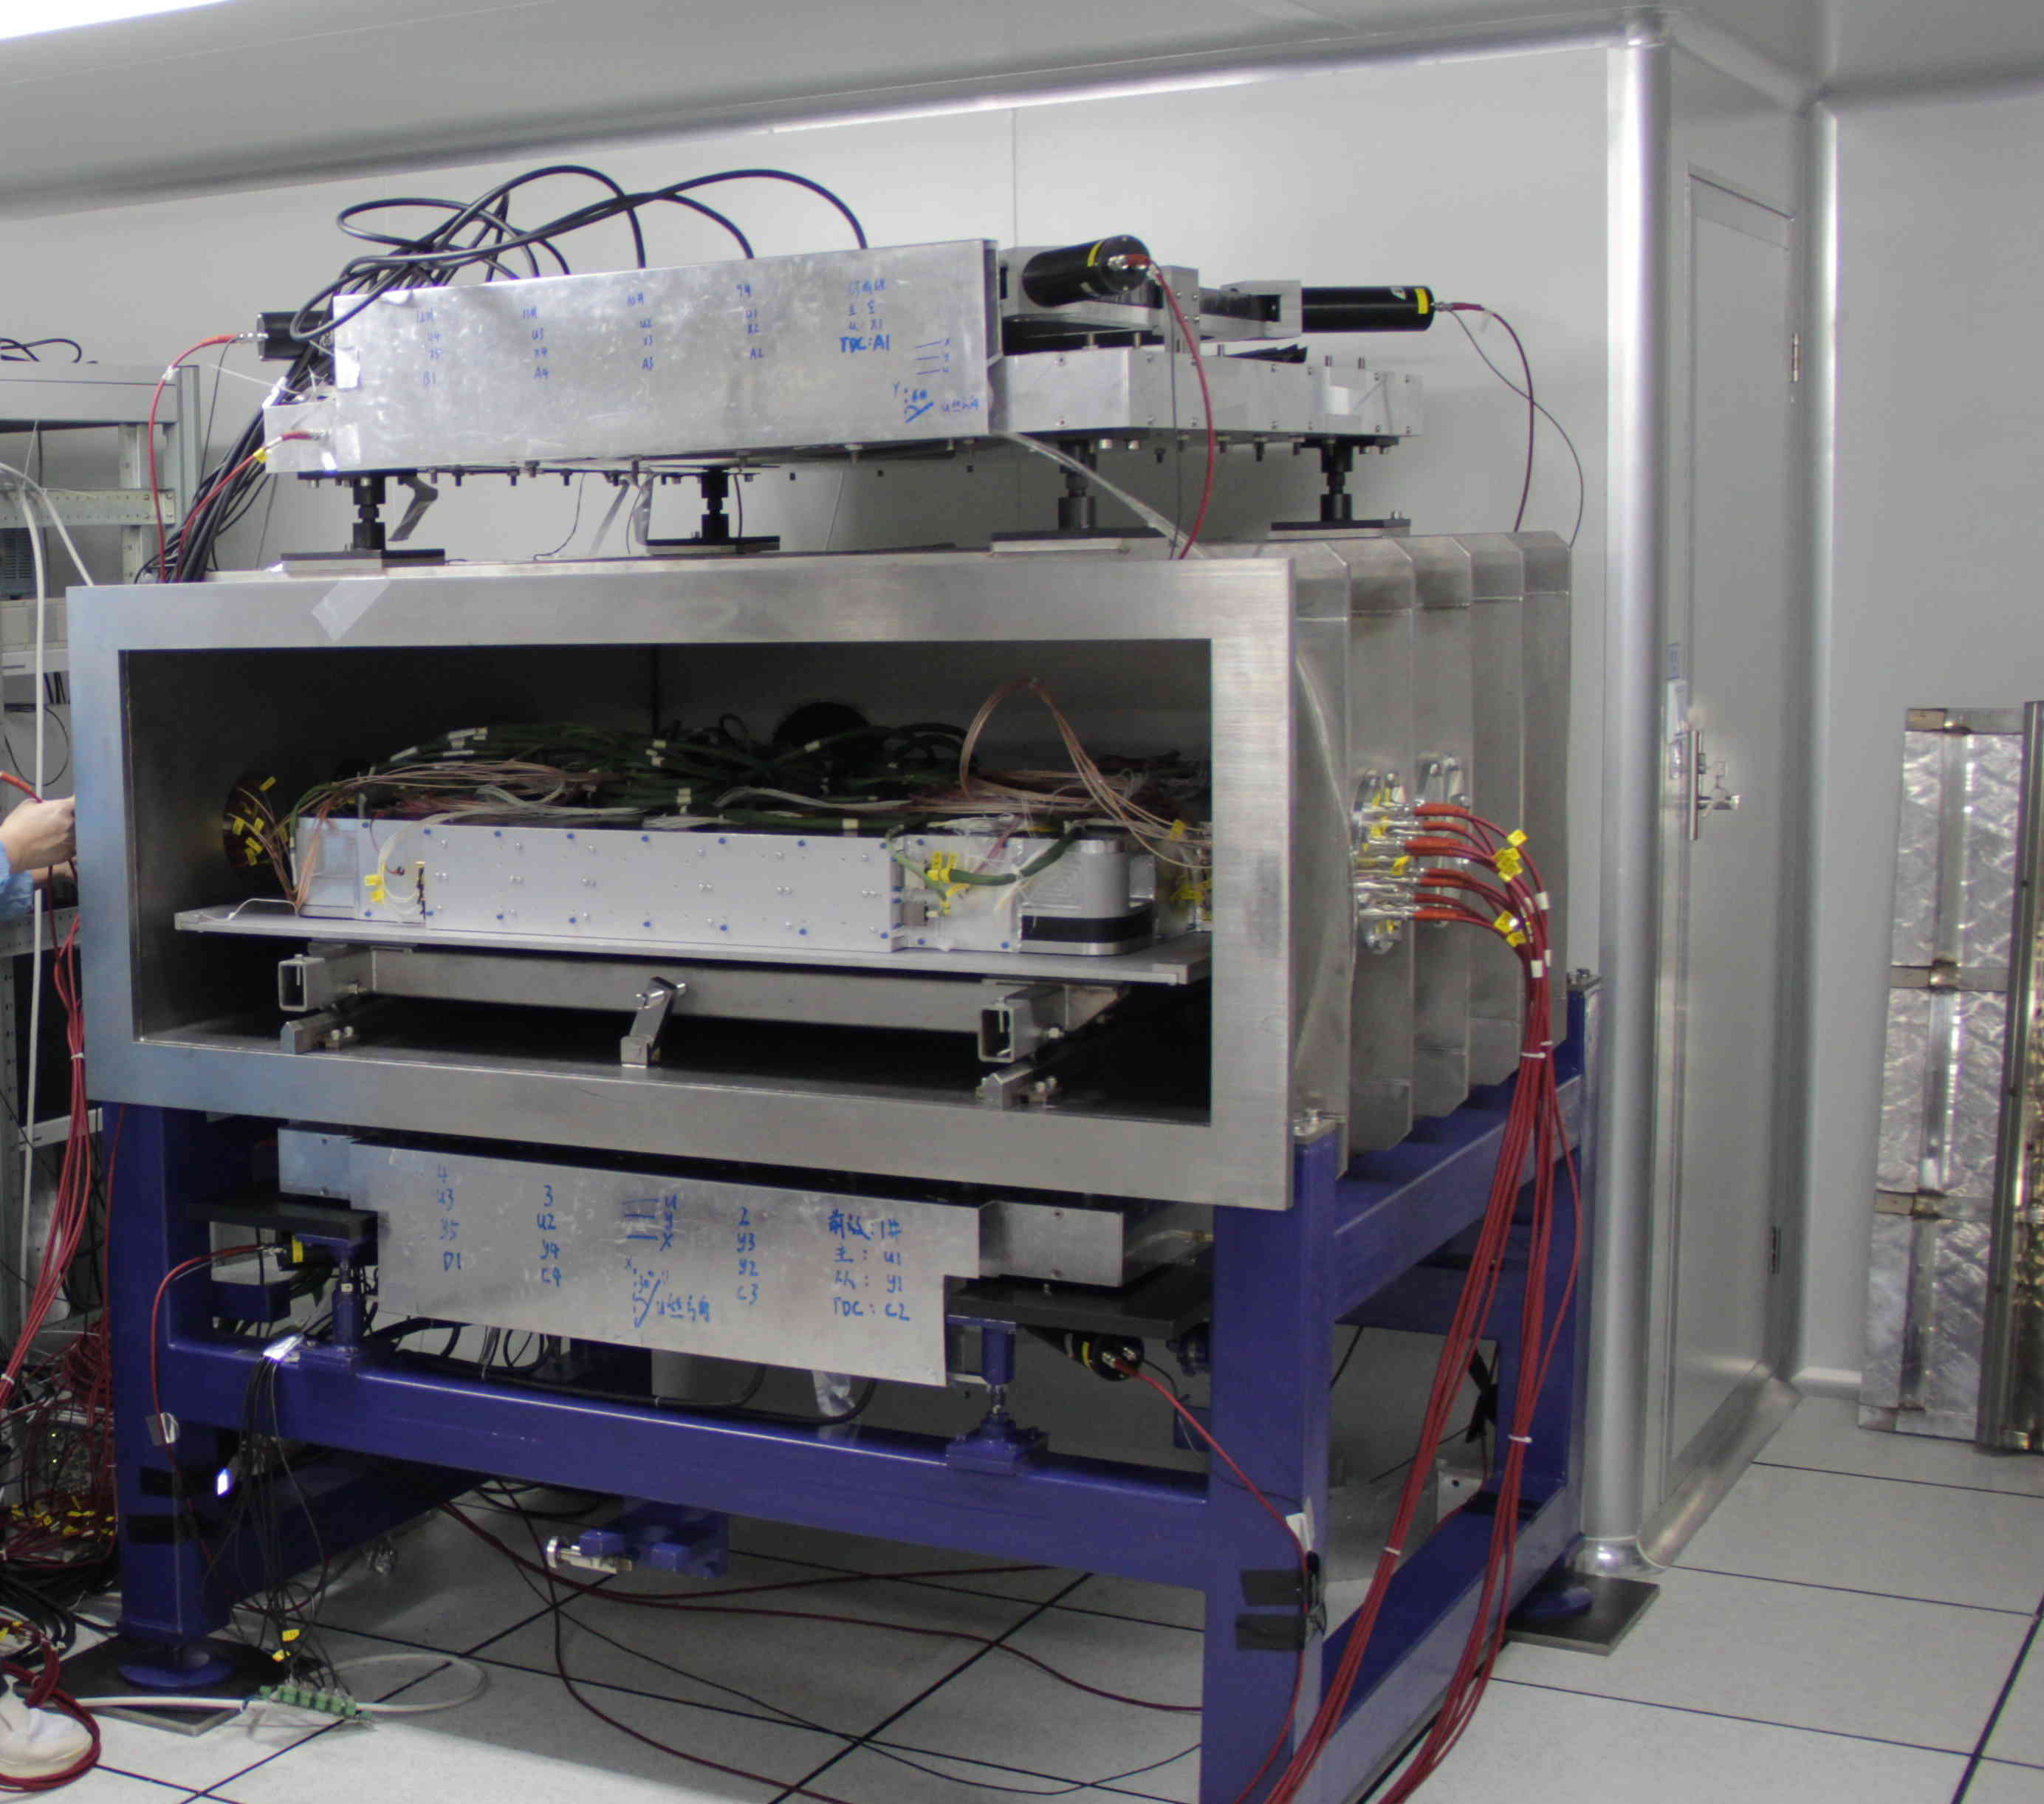
\includegraphics[width=0.65\textwidth]{chap/cosmic_ray/fig/cm_system.jpg}
	\caption{宇宙线地面标定系统的硬件组成}
	\label{fig:cosmic_ray:cm_system}
\end{figure}

按照功能分类,该测试平台可以被分为真空系统、径迹探测系统、触发系统以及数据获取系统四个功能模块。
下面,依次对各个分系统进行详细介绍。

\subsection{真空系统}
\label{sec:cosmic_ray:vacuum_system}
% 靶室大小,结构包括滑台,外观图
% 高压法兰,信号法兰图
% 真空泵,参数
真空系统主要由靶室、真空泵以及真空检测设备组成。
靶室腔体大小为$TODO$,可以容纳整个PSD探测器;靶室外部支架上设计有托盘,用于固定MWDC和塑闪触发板。
靶室内部还铺设了两根导轨,操作时,我们先将PSD安放在一个铝合金滑台上并准确定位,然后将滑台沿着导轨推入到靶室腔体中,最后将滑台用卡扣卡住以防其滑动。这样不仅方便了PSD的放置操作,而且能够准确定位PSD在靶室内部的位置,为后面的数据分析提供依据。
为了给靶室内部的PSD提供高压并将其信号引出,我们专门加工了PSD专用的高压转接法兰和信号转接法兰,如图TODO所示。

真空系统中的真空泵设备由机械泵和分子泵两级组成,以保证靶室内部可以达到较高的真空度。
相应的,真空检测设备也分为TODO。
由于靶室体积较大,我们配备了两套相同的真空泵设备以加快抽真空的速度。
实际使用中发现:当靶室内部放置了PSD探测器和相应的连接线缆后,TODO小时内可以将靶室内部真空抽取最低值多少。

\subsection{径迹探测系统}
\label{sec:cosmic_ray:tracking_system}
% MWDC工作原理
径迹探测系统由两个完全一样的大面积多丝漂移室(MWDC)探测器组成。
MWDC是气体探测器的一种,由于制造成本低廉、操作简单以及位置分辨较高,它是粒子物理实验中最常用的位置灵敏探测器之一。
MWDC一般由多个漂移单元组成,每个漂移单元都是MWDC进行位置测量的最小单位。
一个漂移单元由位于中心的一根阳极丝和周围的若干根阴极丝组成;工作时,阳极丝加正高压(或接地),而阴极丝接地(或加负高压);阴极丝也被称为场丝,因为它们的排布方式决定了漂移单眼内部的电场分布。
入射粒子穿过漂移单元时,在其中发生的物理过程可以叙述如下:
\begin{enumerate}
	\item 入射粒子使得单元内的气体分子电离,从而产生自由的电子离子对。
	\item 在电场作用下,电离出来的电子被加速并缓慢向阳极丝漂移,而离子则向阴极丝移动。
	\item 由于阳极丝附近电场强度非常大,自由电子漂移到这个区域以后迅速被加速到足够高的能量并能够引发新的电离。这个过程不断地反复地进行,从而产生大量电离电子,这个现象被称为雪崩效应。
	\item 雪崩效应产生的自由电子继续向阳极丝移动,由于距离阳极丝非常近,它们立即被阳极丝收集。
	\item 与此同时,原初电离以及次级电离产生的正离子继续向阴极丝移动,由于离子的质量大,它们的漂移速度很慢,而且也不会在阴极丝附近产生雪崩效应。
\end{enumerate}
上述各个步骤中,只有大量雪崩电子向阳极丝移动并被迅速吸收这个过程能够使得阳极丝上的电荷分布发生变化并感应出幅度可探测的电流脉冲信号。
MWDC探测到的也就是这个阳极丝上的感应电流信号,该信号产生时刻与入射粒子穿过漂移单元的时刻的时间差就是原初电离电子的漂移时间。
由于漂移距离与漂移时间直接关联,通过测量漂移时间可以反推出原初电离位置相对于阳极丝的位置,这就是MWDC进行位置测量的基本原理。

% 基本结构:面积,丝参数,精度。
% MWDC结构示意图(丝距离,丝面排布)
% MWDC实物图
宇宙线标定测试平台中使用的MWDC探测器由X,Y,U三个方向的漂移单元平面阵列组成,其有效探测面积为$840mm \times 840mm$。
X面与Y面成\SI{90}{\degree}排布,它们内部都有80个漂移单元;U面与X面成\SI{30}{\degree}排布,它的内部有106个漂移单元,如图\ref{fig:cosmic_ray:mwdc_schematic}中的(a)所示。
漂移单元平面阵列是由两个阴极面和一个阳极面构成的,面间距为\SI{5}{mm}。
其中,阴极面由直径为\SI{100}{\micro\meter}的铍铜丝紧密排列组成,而阳极面由直径为\SI{100}{\micro\meter}的铍铜丝和直径为\SI{20}{\micro\meter}的镀金钨丝间隔排列组成,如图\ref{fig:cosmic_ray:mwdc_schematic}中的(b)所示。
\begin{figure}[htb]
\centering
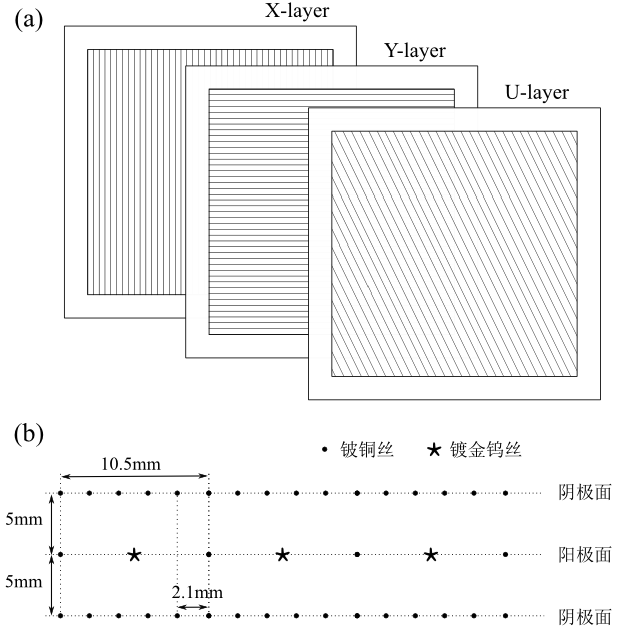
\includegraphics[width=0.65\textwidth]{chap/cosmic_ray/fig/mwdc_schematic.png}
\caption{MWDC内部结构:a)X,Y,U三个方向的漂移单元阵列;b)漂移单元阵列内的丝面排布方式}
\label{fig:cosmic_ray:mwdc_schematic}
\end{figure}
工作时,所有的铍铜丝加负高压,它们是漂移单元的阴极丝;所有的镀金钨丝接地,它们是漂移单元的阳极丝。
因此,根据图\ref{}给出的间距,可以得到MWDC的漂移单元是一个截面为$10mm\times 10.5mm$的长方体。
MWDC探测器的工作气体为$\SI{20}{\percent}CO_2 + \SI{80}{\percent}Ar$,整个漂移腔体用Kapton膜密封,图\ref{fig:cosmic_ray:mwdc}给出了一个MWDC探测器的实物图。
\begin{figure}[htbp]
	\centering
	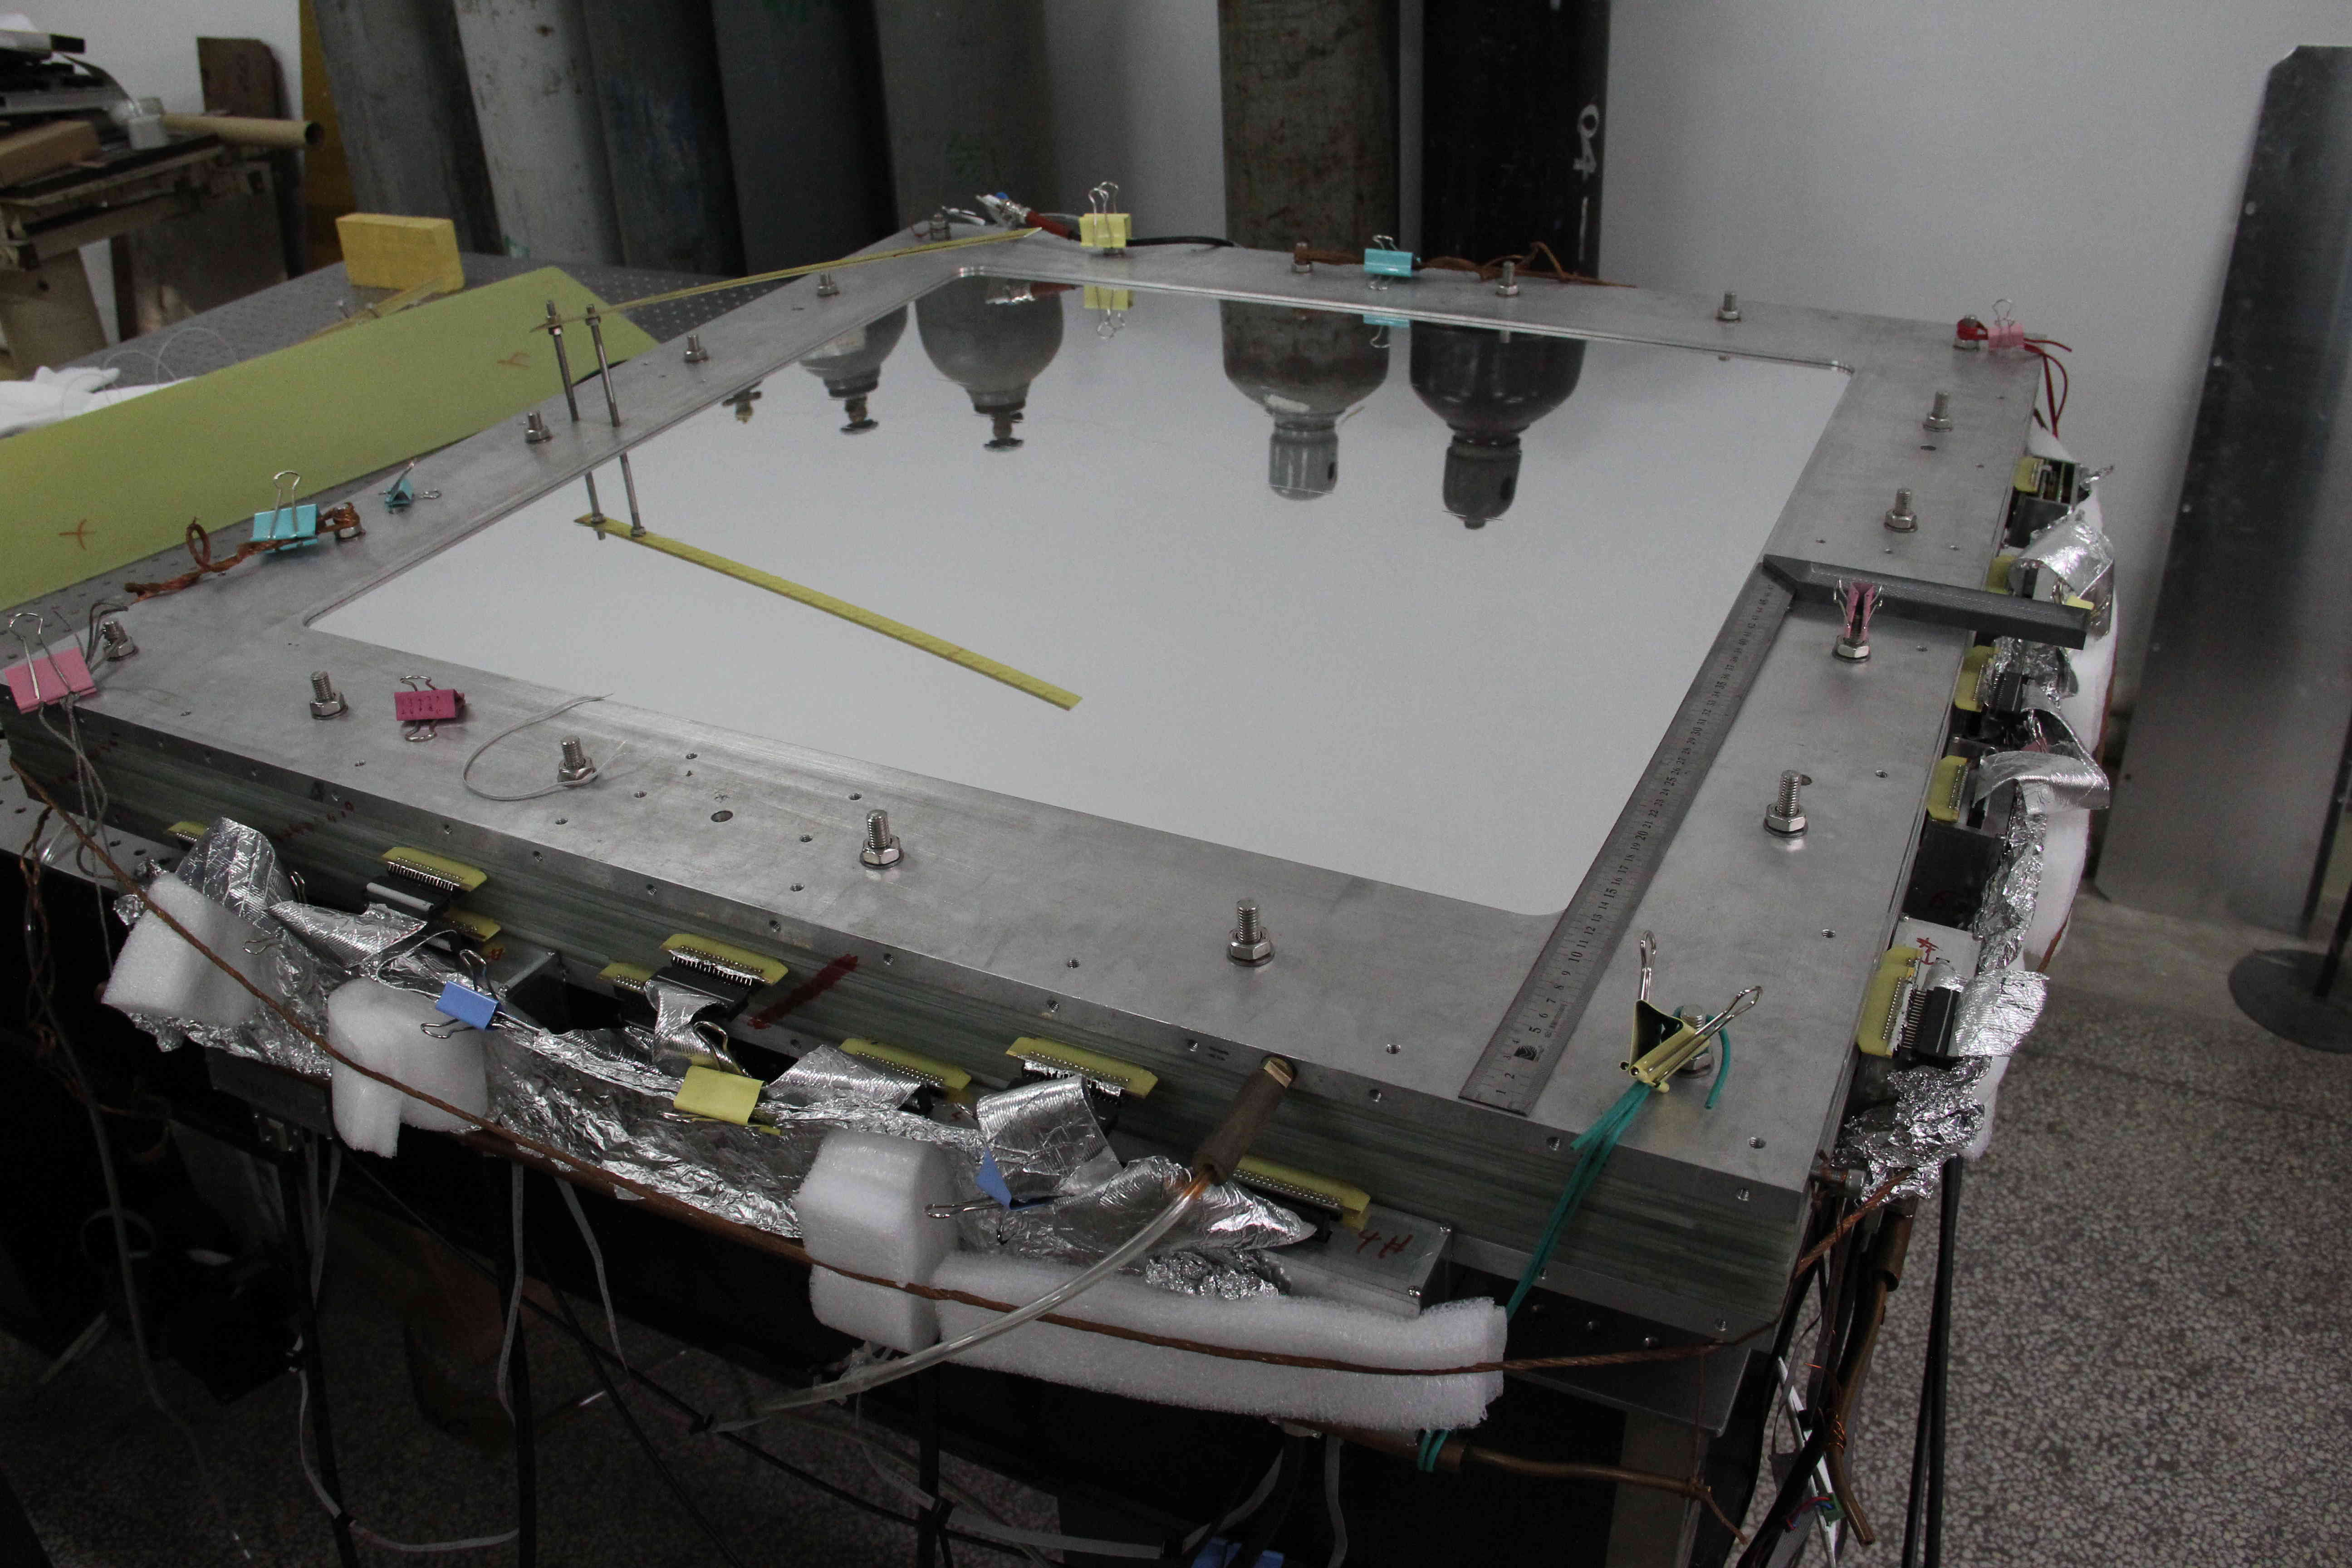
\includegraphics[width=0.65\textwidth]{chap/cosmic_ray/fig/mwdc.jpg}
	\caption{MWDC实物图}
	\label{fig:cosmic_ray:mwdc}
\end{figure}

% MWDC的信号处理系统
MWDC的输出信号幅度较小,为了提高信噪比,我们使用一块基于SFE16芯片的前端电子学板对原始信号进行预处理,然后才将其输出到数据获取系统中进行时间测量(见\ref{sec:cosmic_ray:daq_system}节)。
SFE16是一款专门用于气体漂移室前端信号处理的低噪声ASIC芯片。
它将16个测量通道集成在一块芯片上,每个通道都具有信号放大和甄别的功能,因此输出信号可以直接用于时间测量,并适合长距离传输。
关于SFE16的详细信息可以参考文献\cite{sfe16}。

\subsection{触发系统}
\label{sec:cosmic_ray:triggering_system}
% 触发板结构,面积,厚度,四角读出,实物图?
触发系统由两块完全一样的塑料闪烁体触发板探测器组成。
触发板探测器使用\SI{30}{mm}厚的塑料闪烁体EJ-200\cite{ej-200}作为探测介质,探测器形状为正方形,有效面积为$825mm \times 825mm$。
塑闪板表面抛光,并在内层包裹Tyvek纸以提高反射效率,而在外层包裹黑胶带以屏蔽外界的光干扰。
最后,塑闪板的四个角各耦合了一支光电倍增管,用于闪烁光信号读出,如图TODO所示。
使用的光电倍增管型号为Hamamatsu公司的R7724\cite{r7724}。

% 触发板的信号处理系统
触发系统具有两个功能:1)标识入射宇宙线,为数据获取系统提供触发信号;2)用于宇宙线击中时刻的测量,为MWDC漂移时间的计算提供时间零点。
上下两块触发板探测器共有8路信号输出,相应地,它们经过甄别后可以得到8路时间信号。
每一路时间信号都扇出两路,一路信号参加8路时间信号的逻辑与运算;另一路信号用于时间测量。
上述两个功能都在同一块信号处理板中实现,详细内容参看\ref{sec:cosmic_ray:daq_system}节。
我们认为真实的宇宙线事例应该使得上下两块触发板都点火,因此8路信号相与得到的输出信号将作为触发信号输入到数据获取系统中以记录该事件。
而8个角上得到的时间测量值将被用于漂移时间零点的计算。

% 响应均匀性,击中位置图或者唐述文文章中的图
由于触发板的面积较大,宇宙线击中板上不同位置处产生的闪烁光传输到塑闪板角上PMT的时间是有差异的,我们把这个现象称为时间测量不均匀性,如图\ref{fig:cosmic_ray:tof_timeVSposition}所示。
\begin{figure}[htbp]
	\centering
	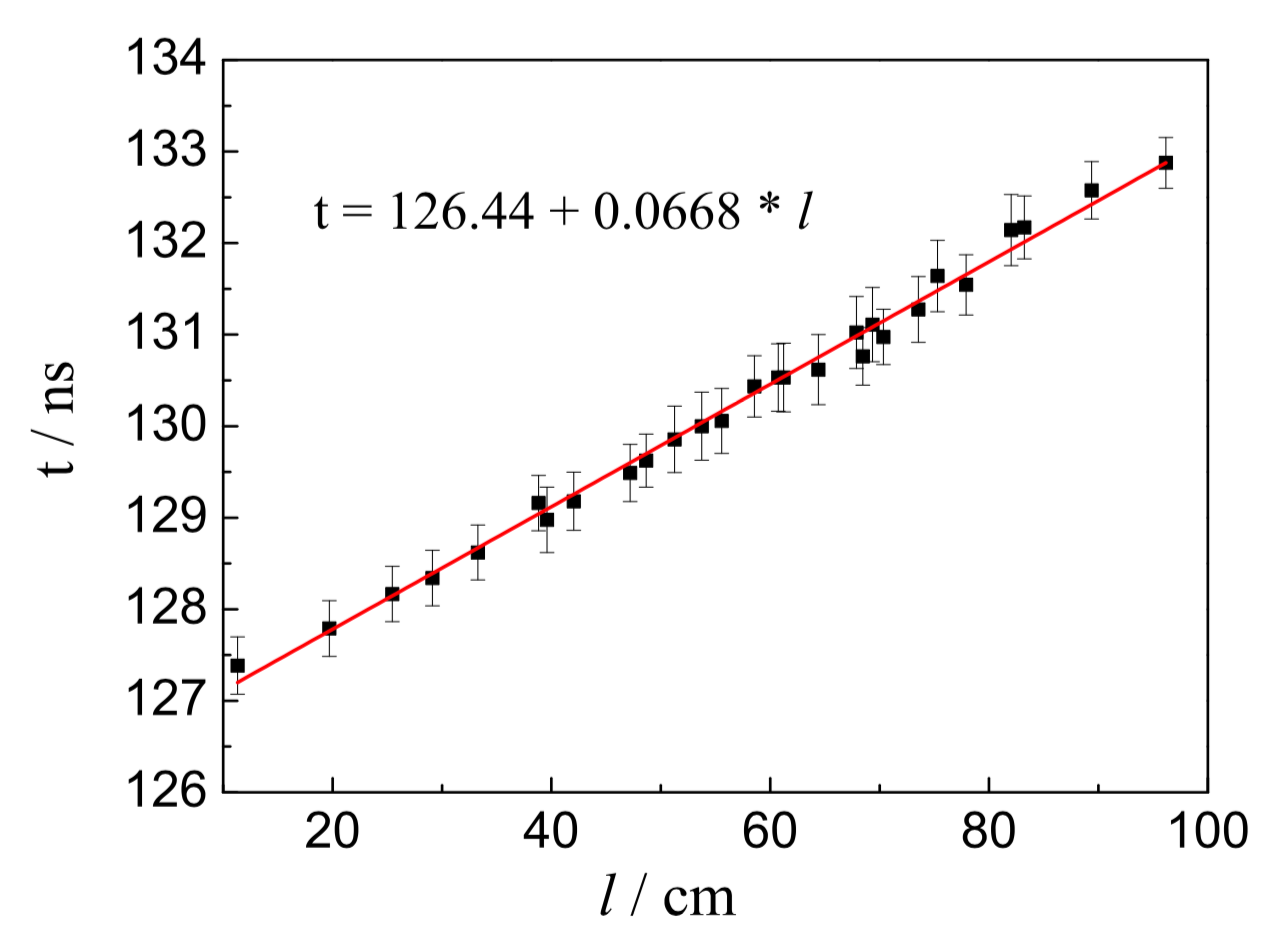
\includegraphics[width=0.65\textwidth]{chap/cosmic_ray/fig/tof_timeVSposition.png}
	\caption{触发板的时间测量不均匀性,引自\cite{tang_large_2015}。其中,纵轴是某个角得到的击中时刻,而横轴是击中位置距离这个角的直线距离。拟合直线斜率的倒数就是闪烁光在塑闪板中的有效传播速度。}
	\label{fig:cosmic_ray:tof_timeVSposition}
\end{figure}
这意味着,我们不能简单地选择一支PMT的时间信号作为时间零点,因为这会带来较大的时间晃动,影响漂移时间的测量精度。
为了消除时间测量不均匀性,必须综合板上四个角的时间测量信息,以使得时间零点与击中位置无关。
实际中,我们使用下列形式\cite{annand_large_1987}得到时间零点$T_{eff}$:
\begin{equation}
	T_{eff} = \frac{1}{4}\sum^4_{i=1}T_i - \frac{v_{eff}}{8d}[(T_3-T_1)^2+(T_4-T_2)^2]
	\label{eq:cosmic_ray:tof_time}
\end{equation}
其中,$v_{eff}$是闪烁光在塑闪板中有效传输速度,$d$是塑闪板的对角线长度,$T_1\sim T_4$是塑闪板四个角的时间测量值,并且$T_1$和$T_3$是对角,而$T_2$和$T_4$也是对角。
测试发现,使用公式\ref{eq:cosmic_ray:tof_time}得到的塑闪板时间分辨率可以达到\SI{350}{\pico\second}\cite{tang_large_2015}。

\subsection{数据获取系统}
\label{sec:cosmic_ray:daq_system}
% PXI机箱图,触发板,MWDC板,TOF板
数据获取系统基于PXI总线设计,主要由触发板,时钟板,TOF测量板以及MWDC测量板组成\cite{kanglongfei_thesis,zhoujiawen_thesis}。
这些板卡都安装在一个6U高,具有15个槽位的PXI机箱中\cite{pxi_chassis},而获取和控制软件安装在机箱第一个槽位的单片机上,如图\ref{TODO}所示。
下面,对这四种板卡的功能进行简单的介绍。

TOF测量板和MWDC测量板是数获取系统进行时间测量的核心模块,其中TOF板用于触发板探测器的时间测量,而MWDC板用于MWDC探测器的时间测量。
两块测量板都是基于HPTDC芯片设计的,能够在高计数率条件下对时间进行精确测量。
HPTDC是欧洲核子中心(CERN)开发的一款高性能时间测量ASIC芯片\cite{TODO}。
与以往核物理实验中常见的起停式时间测量方法不同,HPTDC直接测量输入时间信号的到达时刻,而不是测量输入时间信号与触发信号的时间差。
HPTDC也需要触发信号,但它并不将触发信号作为时间测量的零点,而是使用触发信号来寻找真实的时间测量值,具体流程如下:
\begin{enumerate}
	\item 首先,任何输入到HPTDC的时间信号,不管是真实物理事件产生的还是本底噪声产生的,它们的到达时刻都会被测量并暂时保存到芯片的信号缓存区中。
	\item 之后,触发信号输入到HPTDC中,其到达时刻也被测量并暂时保存到触发信号缓存区中。
	\item 由于触发信号代表真实的物理事件,它的产生时刻与真实待测的时间信号之间必定满足一定的时间关系(包括各种电子学和线缆的延迟时间)。这个关系可以用一个时间窗口来表示,并可以在实验前通过模拟和测试估算出来。用户在实验开始前,需要将这个关系配置保存到在HPTDC的配置寄存器中。
	\item 实验中,HPTDC就是根据这个配置好的时间窗口,从信号缓存区中已有的时间测量值中找到每个触信号对应的真实时间测量值,并将其输出到读取FIFO中,供获取软件使用。
\end{enumerate}
由于HPTDC会将信号缓存区中所有在时间窗口内的测量值都提取出来,因此需要仔细调节时间窗口配置以达到每个触发信号只能找到一个测量值的最佳状态。
这给实验准备提出了更高的要求,但这种测量方法具有死时间小、配置灵活等优点,非常适合复杂探测器系统在高计数率条件下的使用。
HPTDC具有32个测量通道,每个通道的时间测量精度为\SI{98}{\pico\second};HPTDC也可以工作在精度为\SI{25}{\pico\second}的甚高精度模式下,此时每4个测量通道合并成1个测量通道,即此时HPTDC只有8个测量通道。
TOF板共有16个测量通道,其内部共使用了3片HPTDC,其中两片用于时间测量,工作在甚高精度模式下,一片用于TOT幅度测量(Time-Over-Threshold),工作在正常模式下。
MWDC板共有128个测量通道,其内部使用了4片HPTDC,全部工作在正常模式下。

TOF测量板在时间测量模块之前还加入了甄别模块。
这样,来自PMT的原始信号可以直接输入到TOF板中,它们首先经过甄别模块的处理被转换成时间信号,然后才会输入到HPTDC芯片中。
而MWDC测量板不需要添加额外的甄别模块,因为MWDC探测器原始信号的甄别工作在前端电子板中就已经完成(见\ref{sec:cosmic_ray:tracking_system}节)。
另外,TOF测量板还能够依次对相邻两路输入通道的时间信号做逻辑与运算,然后将得到的8个与运算结果再作或运算,并将最终结果从前面板输出。

由于HPTDC只能测量时刻值,为了得到漂移时间,我们需要将MWDC板测得的信号时刻减去TOF板测得的宇宙线击中时刻。
这就要求不同测量板内的HPTDC芯片参考时钟是同步的,这样我们才能将不同测量板的时间测量结果直接相减。
时钟板的功能就是输出16路完全同步的\SI{40}{Hz}时钟信号。
这些时钟信号通过等长的时钟信号线缆输入到每块测量板中,这样所有测量板就有了统一的参考时钟信号,它们的测量结果也就能够直接进行对比了。

触发板主要有两个功能:1)接收外部触发信号,然后将该触发信号同步地分发到各块测量板中;2)将HPTDC的时间重置命令同步发送到各块测量板。
其中,时间重置命令的同步发送对不同测量板的时间测量同步性至关重要。
为了保证严格的同步性,触发板安装在PXI机箱的2号槽位中,并使用PXI机箱背板上的星形触发总线来进行触发信号
和时间重置信号的分发。
星形触发(Star Trigger)是PXI总线的主要特点之一,PXI机箱的第二个槽位是星形触发控制器槽,该槽位到达其它13个槽位的走线长度是等长的,因此可以实现信号分发严格同步。

% \section{多丝漂移室的宇宙线刻度}
% \subsection{漂移时间零点的确定}
% \subsection{从漂移时间谱提取s-t关系:Integration Method}
% \subsection{迭代修正s-t关系}
% \subsection{多丝漂移室的性能参数}

\section{PSD的宇宙线标定测试配置}

% 15天,23个/s,一共事例数? 27%左右的单根丝点火事例
我们使用上述宇宙线地面标定系统对PSD进行了长达半个月的宇宙线标定测试。
测试时,PSD被安置在真空靶室中,靶室内真空度一直保持在TODO,PSD的各探测单元模块加载额定工作电压。
整个测试期间,PSD各功能模块工作稳定,也没有发现PSD发生高压打火的现象。

% 与PSD系统的集成,触发Veto板。
PSD和宇宙线标定测试平台的数据获取系统在硬件和软件上都是完全独立的,两者各自获取一份数据并保存在不同的计算机中,如图\ref{fig:cosmic_ray:cm_test}所示。
\label{sec:cosmic_ray:cm_test}
\begin{figure}[htbp]
	\centering
	\includegraphics[width=0.65\textwidth]{chap/cosmic_ray/fig/cm_test.jpg}
	\caption{PSD的宇宙线标定测试}
	\label{fig:cosmic_ray:cm_test}
\end{figure}
这就涉及到两个系统的同步问题:我们将同一个触发信号同时分发到两个获取系统中,并期望两者能够同时处理完这个事例,并一起等待下个触发信号的到来。
为此,我们开发了一块触发Veto板,它接收来自触发系统的宇宙线触发信号,然后将其扇出两路,并分别输出到PSD
和宇宙线标定测试平台的数据获取系统中。
与一般的触发分发不同的是,该触发Veto板在接收一个有效触发信号并分发出去后,它在一定的时间间隔内不再接收新的触发信号,即屏蔽这段时间内的所有宇宙线触发事例。
如果将这个屏蔽时间设置为两个获取系统的最大死时间,我们就可以保证两个系统在接收到下个触发信号前都完成了前一个事例的处理,从而强制实现了两者的同步。
这种同步方法是被动的,如果屏蔽时间设置的过大,就可能导致部分有效事例丢失。
实际中,我们将触发Veto板的屏蔽时间设置为\SI{1}{ms},即PSD获取系统的死时间。
由于宇宙线事例的触发率远小于\SI{1000}{\per\second},该屏蔽时间设置基本不会导致事例丢失。

% 触发板预支设置,击中分布图
测试前,我们还对触发系统的8个读出PMT的工作电压进行了调节和测,原则是:1)在不增加噪声的前提下,尽量升高PMT的工作电压,提高增益系数,达到提高触发效率的目的;2)调节同一块触发板4个角读出PMT的电压,使得它们的增益基本一致,达到不同击中位置的触发效率基本一致的目的。
最终,在实际测试中,触发系统的宇宙线触发效率达到了\SI{27}{\per\second},并实现了较好的触发效率均匀性。
图\ref{fig:cosmic_ray:hitposition}给出了靶室上方MWDC探测器的宇宙线击中位置分布图以及重建径迹在PSD上的击中位置分布图,靶室下方MWDC探测器也有类似结果。
\begin{figure}[htb]
\centering
\subfloat[][MWDC的宇宙线击中位置分布]{
	\label{fig:cosmic_ray:hitposition_mwdc}
	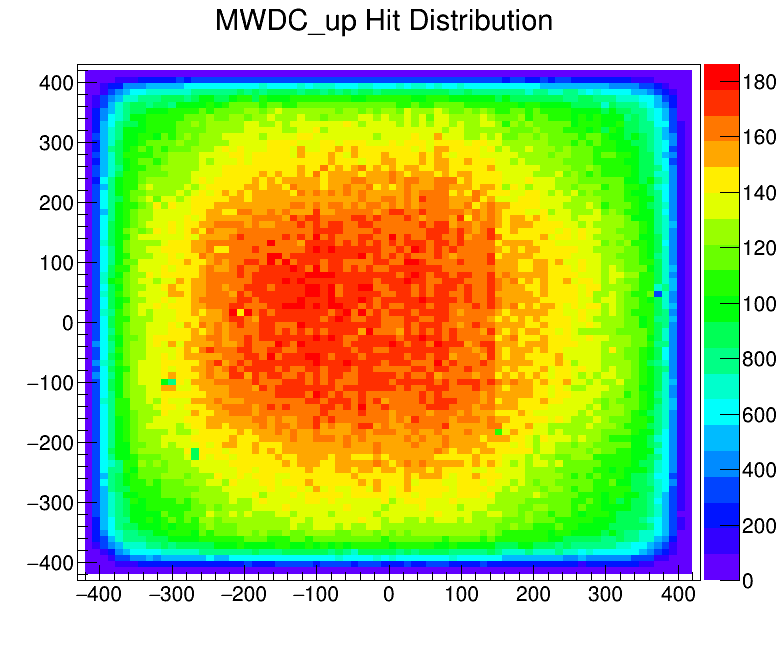
\includegraphics[width=0.48\textwidth]{chap/cosmic_ray/fig/hitposition_mwdc.png}
}
% \hfill
\subfloat[][PSD的宇宙线击中位置分布]{
	\label{fig:cosmic_ray:hitposition_psd}
	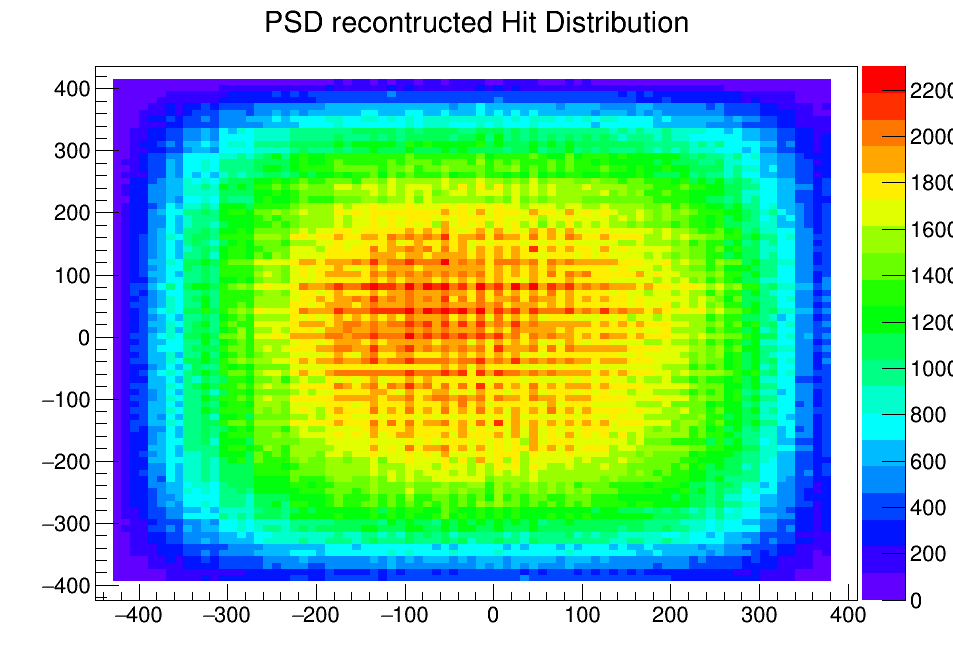
\includegraphics[width=0.48\textwidth]{chap/cosmic_ray/fig/hitposition_psd.png}
}
\caption{触发系统的触发效率均匀性}
\label{fig:cosmic_ray:hitposition}
\end{figure}
可以看到,击中位置分布呈现出中间多,边缘少的特点,这是因为两块触发板距离较远,中间位置的接收角度远大于边缘位置。
同时可以看到,击中位置在四周,尤其是4个角上的分布基本均匀,这说明不同位置处的触发效率基本是一致的。

\section{PSD的宇宙线标定结果}
\label{sec:cosmic_ray:results}
\subsection{基线噪声}
加高压与未加高压的结果对比。
基线中心值。
电子学刻度?

\subsection{MIP响应}
中心MIP拟合示例图
中心值一致性
能量分辨率分布

\subsection{光衰减效应}

\subsection{Dy58比值}
拟合示例
分布图,与LED测试值对比
动态范围计算与分布

\subsection{探测效率}
探测效率判据
事例筛选
结果分布

\subsection{位置分辨}
位置重建原理
结果

\section{PSD的物理量重建研究}
\subsection{能量重建}
\subsection{位置重建}
	% 各章节。
	% \chapter{PSD在CERN-SPS的重离子束流标定}

\section{实验简介}
\subsection{实验条件}
\subsection{辅助探测器与实验布局}
\subsection{次级束的产生}
\subsection{$\Delta E$-$\Delta E$重离子鉴别方法}
\subsection{数据分析}

\section{PSD的重离子响应}
\subsection{Dynode8/Dynode5比值的线性}
\subsection{重离子的光输出}
\subsection{光衰减效应}
\subsection{不同单元模块的响应均匀性}

\section{PSD的电荷分辨能力}
\subsection{单元模块的电荷分辨率}
\subsection{PSD整体的刻度与能量重建}
\subsection{PSD的电荷自分辨}

\section{结论}
	% 结论
	% vim:ts=4:sw=4
% Copyright (c) 2014 Casper Ti. Vector
% Public domain.

\chapter{总结与展望}
\label{ch:conclusion}

\section{总结}

DAMPE卫星自2015年12月17日发射并进入轨道后,已经完成了三个月的在轨测试阶段,并正式进入到巡天观测模式。
在轨测试期间,PSD探测器整体工作正常,各项性能指标符合设计要求并非常稳定,从而验证了PSD的设计合理性,并说明PSD建造过程的质量控制过关。

本论文完整展现了PSD从整体设计、组件原理验证、探测器建造以及宇宙线标定的整个研制过程。
其中,论文的主要工作集中在细致研究了影响PSD探测性能的几个关键技术,完成了PSD的建造,并对PSD整体进行了地面宇宙线标定。
另外,论文工作过程中还完成了两套大型的探测器辅助测试平台的设计和研制,这些测试平台为PSD的研制成功提供了坚实的基础。
下面,对本论文取得的主要成果进行一个小结:
\begin{enumerate}
	\item PSD关键技术的细致研究:
	\begin{itemize}
		\item PSD需要覆盖接近4个量级的动态范围区间,这是PSD探测器主体功能模块的主要设计难点。本论文完成了基于Dy5和Dy8双打拿极信号引出的大动态范围读出方案的设计与实验验证,结果显示该设计方案能够满足PSD的动态范围要,并最终应用到PSD的正样飞行件上。
		\item PMT的工作状态直接关系到PSD探测单元模块的性能,大规模的探测器系统中往往需要对大量的PMT进行测试并进行筛选,对于PSD来说此项筛选流程更加严格。本论文对570支候选R4443裸管进行了测试,使用相对增益测量方法得到了它们的增益特性曲线,同时也得到了绝对的Dy58比值增益特性曲线。根据PSD的特殊要求,本论文确定了严格的筛选条件,并根据PMT的测试结果进一步从570支PMT中挑选出164支安装到PSD上。
	\end{itemize}
	\item PSD的建造:探测器的建造相对来讲是一个较为琐碎的过程,然后PSD的建造过程中涉及了大量的工艺和质量测试程序,使得它可以单独成为一个系统,并直接决定PSD最终的探测器性能。本论文的工作完整参与了PSD的整个建造流程。
	\item PSD的宇宙线测试:本论文对装配完成的PSD进行了长度15天的宇宙线测试,并从中提取除了PSD的性能参数,发现PSD的实际性能达到并好于设计指标;另外,本文还从宇宙线标定数据中提取出了PSD的第一批刻度数据,这些数据对于研究PSD的能量重建和模拟具有重要价值。
	\item 大型辅助测试平台的研制:
	\begin{itemize}
		\item PMT批量测试平台是本论文为PSD的R4443测试专门设计和建造的,它最多能够同时测量25支PMT,并具有光阴极扫描功能。考虑到在日常的探测器研制过程经常会有PMT测试工作,本论文对该平台采用模块化设计,其硬件组件和软件组件都很容易更换或更新以适应新的应用需求。
		\item 地面宇宙线标定测试平台是本论文为PSD的宇宙线标定专门设计和建造的,并用它完成了PSD的初次宇宙线刻度。同样的,该测试平台也适合在其它探测器的研制过程中使用。
	\end{itemize}
\end{enumerate}

\section{展望}
PSD的研制工作随着DAMPE的发射成功以及在轨测试的顺利完成而圆满结束。
现在,DAMPE已经进入正式的物理观测模式,每天都是大量的数据下传,同时也意味着对PSD的研究中心将转向物理量的精细重建上,主要有:
\begin{enumerate}
	\item 完成PSD每个探测单元模块的精细能量重建,包括光衰减效应的修正,两端的能量信息提取及综合等。
	\item 完成PSD探测器整体的能量重建,包括击中交叠单元模块的事件处理,量能器反照粒子的干扰去除等。
	\item 完成PSD的Geant4模拟中的数字化工作。
	\item 实现PSD的$e/\gamma$分辨算法,这需要利用STK的重建径迹以及BGO的簇射形状重建。
	\item 完成PSD的在轨标定工作,包括MIPs响应,Dy58比值,电子学刻度,基线以及这些量随环境参数的变化等。
\end{enumerate}

	% special chapter没有章节编号,在目录中显示
% 	\subimport*{chap/special}{}
	% 正文中的附录部分。
	\appendix
	% 排版参考文献列表。
	\printbibliography[
		% 使“参考文献”出现在目录中;如果同时要使参考文献列表参与章节编号,
		% 可将“bibintoc”改为“bibnumbered”。
		heading = bibintoc,
		% 单独设定排序方案。此设定会局部覆盖之前的全局设置。
		% 注:只有同时使用 2.x 或之后版本的 biblatex 和相应兼容版本的 biber,
		% 才能对每个 \printbibliography 命令采用不同的排序方案,
		% 否则只能在载入 biblatex 宏包时就(全局)指定排序方案。
		% 在这样的情况下,请去掉所有的 sorting 选项,否则可能出错。
		% 此外,biblatex 3.0 中 \printbibliography 的 sorting 选项失效,
		% 详见 biblatex-caspervector 的文档。
		sorting = ecnty
	]
	% 各附录。
	% % vim:ts=4:sw=4
% Copyright (c) 2014 Casper Ti. Vector
% Public domain.

\chapter{PMT批量测试平台测控软件平台的设计}
\label{appendix:pmttest_software}

\begin{figure}[htbp]
	\centering
	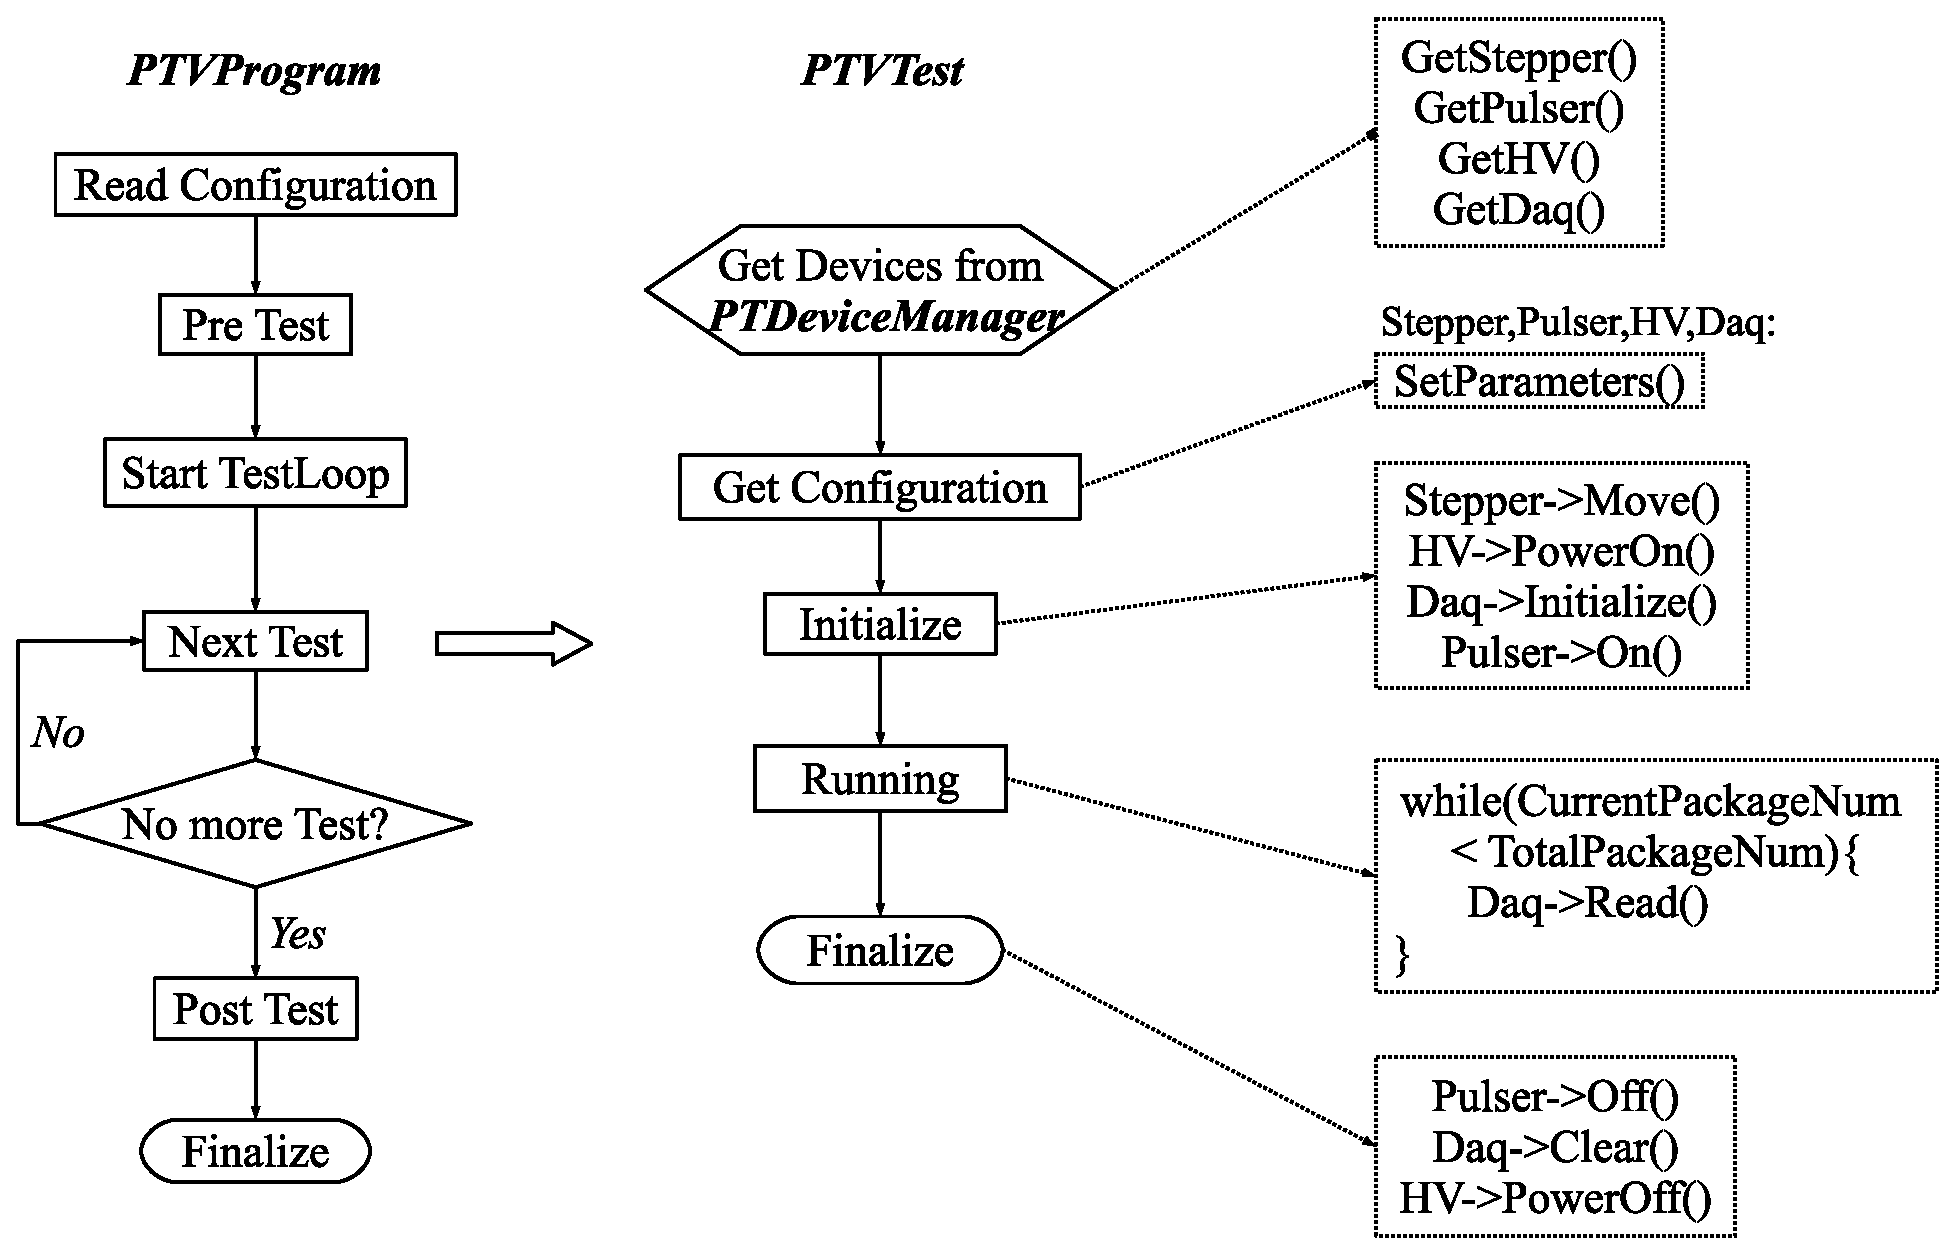
\includegraphics[width=0.9\textwidth]{chap/pmt_test/fig/software_framework.eps}
	\caption{软件框架框图}
	\label{fig:pmt_test:software_framework}
\end{figure}
	%\chapter{基于HPTDC的高精度时间测量}
	
	
	% 以下为正文之后的部分,默认不进行章节编号。
	\backmatter
	
\end{document}

